\documentclass[11pt,twoside,a4paper]{book}  
% definice dokumentu
\usepackage[czech, english]{babel}
\usepackage[T1]{fontenc} 				% pouzije EC fonty 
\usepackage[utf8]{inputenc} 			% utf8 kódování vstupu 
\usepackage[square, numbers]{natbib}	% sazba pouzite literatury
\usepackage{indentfirst} 				% 1. odstavec jako v~cestine, pro práci v~aj možno zakomentovat
\usepackage{fancyhdr}					% tisk hlaviček a~patiček stránek
\usepackage{nomencl} 					% umožňuje snadno definovat zkratky a~jejich seznam

%%%%%%%%%%%%%%%%%%%%%%%%%%%%%%%%%%%%%%%%%%%%%%%%%%%%%%%%%%%%%%%
% informace o práci
\newcommand\WorkTitle{Software pro distribuované řízení a vyčítání dat ze sítě částicových pixelových detektorů Timepix3} % název
\newcommand\FirstandFamilyName{Bc. Jakub Begera} % autor
\newcommand\Supervisor{Ing. Štěpán Polanský} % vedoucí

\newcommand\TypeOfWork{Diplomová práce}	% typ práce [Diplomová práce | Bakalářská práce | Bachelor's Project | Master's Thesis ]	

% Nastavte následují podle vašeho oboru a~programu (pomoc hledejte na http://www.fel.cvut.cz/cz/education/bk/prehled.html)								
\newcommand\StudProgram{Otevřená informatika} % program
\newcommand\StudBranch{Softwarové inženýrství} % obor

%%%%%%%%%%%%%%%%%%%%%%%%%%%%%%%%%%%%%%%%%%%%%%%%%%%%%%%%%%%%%%%
% minimální importy
\usepackage{graphicx}					% pro vkládání obrázků
\usepackage{k336_thesis_macros} 		% specialni makra pro formatovani DP a~BP
\usepackage[
pdftitle={\WorkTitle},				% nastaví v~informacích o pdf název
pdfauthor={\FirstandFamilyName},	% nastaví v~informacích o pdf autora
colorlinks=true,					% před tiskem doporučujeme nastavit na false, aby odkazy a~url nebyly šedé při ČB tisku
breaklinks=true,
urlcolor=red,
citecolor=blue,
linkcolor=blue,
unicode=true,
]
{hyperref}								% pro zobrazování "prokliknutelných" linků 

% rozšiřující importy
\usepackage{listings} 			%slouží pro tisk zdrojových kódů se syntax higlighting
\usepackage{algorithmicx} 		%slouží pro zápis algoritmů
\usepackage{algpseudocode} 		%slouží pro výpis pseudokódu
\usepackage{inconsolata}		%monospace font
\usepackage{soul}				%zvýrazňovač
\usepackage[final]{pdfpages}    %PDF include
\usepackage{subcaption}			%pro reference na subfigures 
\usepackage{enumitem}
\usepackage{bytefield}
\usepackage{pgf-umlsd}			%sekvenční UML diagramy
\usepackage{tikz}		        %TeX obrázky
\usetikzlibrary{trees,calc,positioning,shapes.geometric,matrix,arrows,decorations.pathreplacing,arrows.meta,decorations.markings,math}

\usepackage{minted}				% slouží k~Syntax Highlighting
\usepackage{amsmath}

\usepackage{forest}
\definecolor{folderbg}{RGB}{124,166,198}
\definecolor{folderborder}{RGB}{110,144,169}
\definecolor{cvut_color}{RGB}{3,46,85}
\definecolor{blue_ligh}{RGB}{0,118,203}

\def\Size{4pt}
\tikzset{
  folder/.pic={
    \filldraw[draw=folderborder,top color=folderbg!50,bottom color=folderbg]
      (-1.05*\Size,0.2\Size+5pt) rectangle ++(.75*\Size,-0.2\Size-5pt);  
    \filldraw[draw=folderborder,top color=folderbg!50,bottom color=folderbg]
      (-1.15*\Size,-\Size) rectangle (1.15*\Size,\Size);
  }
}

%%%%%%%%%%%%%%%%%%%%%%%%%%%%%%%%%%%%%%%%%%%%%%%%%%%%%%%%%%%%%%%
% příkazy šablony
\makenomenclature								% při překladu zajistí vytvoření pracovního souboru se seznamem zkratek
% zkratky CERN + ČVUT
\nomenclature{CERN}{Evropská organizace pro jaderný výzkum (Originální název: \textit{Conseil Européen pour la Recherche Nucléaire}), se sídlem v Ženevě, ve Švýcarsku.}
\nomenclature{ATLAS}{A Toroidal LHC Apparatus}
\nomenclature{LHC}{Large Hadron Collider}
\nomenclature{LS}{Long Shutdown - dlouhodobá technologická přestávka LHC}
\nomenclature{DCS}{Detector Control Systems}
\nomenclature{DSS}{Detector Safety System}
\nomenclature{DAQ}{Data Acquisition System}
\nomenclature{ÚTEF}{Ústav technické a experimentální fyziky}
\nomenclature{SATRAM}{Space Application of Timepix based Radiation Monitor}

% detektory
\nomenclature{TPX}{Timepix}
\nomenclature{MPX}{Medipix}
\nomenclature{TOT}{Time Over Treshold - mód detektoru (viz \ref{det:mod})}
\nomenclature{ToA}{Time of Arrival - mód detektoru (viz \ref{det:mod})}
\nomenclature{ASIC}{Application-specific Integrated Circuit}
\nomenclature{FPGA}{Field Programmable Gate Array}
\nomenclature{DAC}{Digitálně analogový převodník}
\nomenclature{ADC}{Analogově digitální převodník}
\nomenclature{CMOS}{Complementary Metal Oxide Semiconductor}
\nomenclature{CSM}{Charge Summing Mode}
\nomenclature{FITPix}{Fast Interface for Timepix Pixel Detectors}
\nomenclature{LVDS}{Low-voltage differential signaling}
\nomenclature{PCC}{Photon Counting Chip}
\nomenclature{ISO}{International Organization for Standardization}
\nomenclature{OSI}{Open Systems Interconnection model}

% software & hardware & elektronika
\nomenclature{HTTPS}{Hypertext Transfer Protocol Secure}
\nomenclature{HTTP}{Hypertext Transfer Protocol}
\nomenclature{API}{Application Programming Interface}
\nomenclature{REST}{Representational State Transfer}
\nomenclature{JSON}{JavaScript Object Notation}
\nomenclature{SQL}{Structured Query Language}
\nomenclature{URL}{Uniform Resource Locator}
\nomenclature{b}{bite}
\nomenclature{B}{byte}
\nomenclature{PC}{Personal Computer}
\nomenclature{HW}{Hardware}
\nomenclature{SW}{Software}
\nomenclature{USB}{Universal Serial Bus}
\nomenclature{PN}{Přechod polovodiče typu P a polovodiče typu N}
\nomenclature{TCP}{Transmission Control Protocol}
\nomenclature{IP}{Internet Protocol}
\nomenclature{SSH}{Secure Shell}
\nomenclature{PCB}{Printed Circuit Board}
\nomenclature{SPI}{Serial Peripheral Interface}
\nomenclature{GPIO}{General Purpose Input/Output}
\nomenclature{UDP}{User Datagram Protocol}
\nomenclature{SFTP}{Secure File Transfer Protocol}
\nomenclature{HDFS}{Hadoop Distributed File System}
\nomenclature{DOM}{Document Object Model}
\nomenclature{DSL}{Domain-specific language}
\nomenclature{J2EE}{Java Enterprise Edition}
\nomenclature{JPA}{Java Persistent API}
\nomenclature{JAR}{Java Archive}
\nomenclature{WAR}{Web Application Archive}
\nomenclature{BSON}{Binární forma JSON}
\nomenclature{JSON}{JavaScript Object Notation}
\nomenclature{REST}{Representational State Transfer}
\nomenclature{ID}{Identifikátor}
\nomenclature{LOB}{Large Object}
\nomenclature{CRUD}{Create, read, update and delete}
\nomenclature{HTML}{Hypertext Markup Language}
\nomenclature{MVC}{Model View Controller}
\nomenclature{ACQ}{Datagram typu acknowledge}
\nomenclature{ASCII}{American Standard Code for Information Interchange}
\nomenclature{UTC}{Koordinovaný světový čas (anglicky Coordinated Universal Time)}
\nomenclature{ORM}{Object-relational mapping}
\nomenclature{JRE}{Java Runtime Environment}
\nomenclature{CSS}{Cascading Style Sheets}
\nomenclature{JS}{JavaScript}

% matematické zkratky
\nomenclature{FWHM}{Full width at half maximum}

% fyzikální a chemické zkratky
\nomenclature{eV}{elektronvolt}
\nomenclature{GaAs}{Arsenid gallitý}
\nomenclature{CdTe}{Cadmium telluride}
\nomenclature{Si}{Křemík}
\nomenclature{In}{Indium}
\nomenclature{Fe}{Železo}
\nomenclature{Cu}{Hliník}


\let\oldUrl\url									% url adresy budou zobrazeny: <url> 
\renewcommand\url[1]{<\texttt{\oldUrl{#1}}>}
%\renewcommand\lstlistingname{Výpis kódu} % předefinování nadpisu
%\renewcommand\lstlistlistingname{Výpisy kódu} % předefinování nadpisu v~obsahu
%\renewcommand{\lstlistingname}{Algorithm}% Listing -> Algorithm
%\renewcommand{\lstlistlistingname}{Listdassad of \lstlistingname s}% List of Listings -> List
%%%%%%%%%%%%%%%%%%%%%%%%%%%%%%%%%%%%%%%%%%%%%%%%%%%%%%%%%%%%%%%
% vaše vlastní příkazy
\newcommand*{\nomExpl}[2]{#2 (#1)\nomenclature{#1}{#2}} % usnadňuje zápis zkratek : Slova ke Zkrácení (SZ)
\newcommand*{\nom}[2]{#1\nomenclature{#1}{#2}} % usnadňuje zápis zkratek : SZ
\newcommand*{\todo}{\hl{\textbf{TODO}}} % pro poznámky
\newcommand{\addbibresource}[1]{}
\newcommand*{\footnoteUrl}[1]{\footnote{\url{#1}}}
\newcommand{\unit}[2]{$#1~\ensuremath{\mathrm{#2}}$} % pro jednotky

% custom padding
\def\changemargin#1#2{\list{}{\rightmargin#2\leftmargin#1}\item[]}
\let\endchangemargin=\endlist 

\usepackage{caption}
\DeclareCaptionType{code}[Zdrojový kód][Seznam zdrojových kódů] 
%%%%%%%%%%%%%%%%%%%%%%%%%%%%%%%%%%%%%%%%%%%%%%%%%%%%%%%%%%%%%%%
% vlastní dokument
%%%%%%%%%%%%%%%%%%%%%%%%%%%%%%%%%%%%%%%%%%%%%%%%%%%%%%%%%%%%%%%
\begin{document}

	%%%%%%%%%%%%%%%%%%%%%%%%%% 
	% nastavení jazyka, kterým je práce psána
	\selectlanguage{czech}	% podle jazyka práce nastavte na [czech | english]
	\translate				% nastaví české nebo anglické popisy (např. katedra -> department); viz k336_thesis_macros


	%%%%%%%%%%%%%%%%%%%%%%%%%%    
	% Titulni stranka / Title page 
	\coverpagestarts

	%%%%%%%%%%%%%%%%%%%%%%%%%%    
	% Zadani / Assignment
	\newpage~
	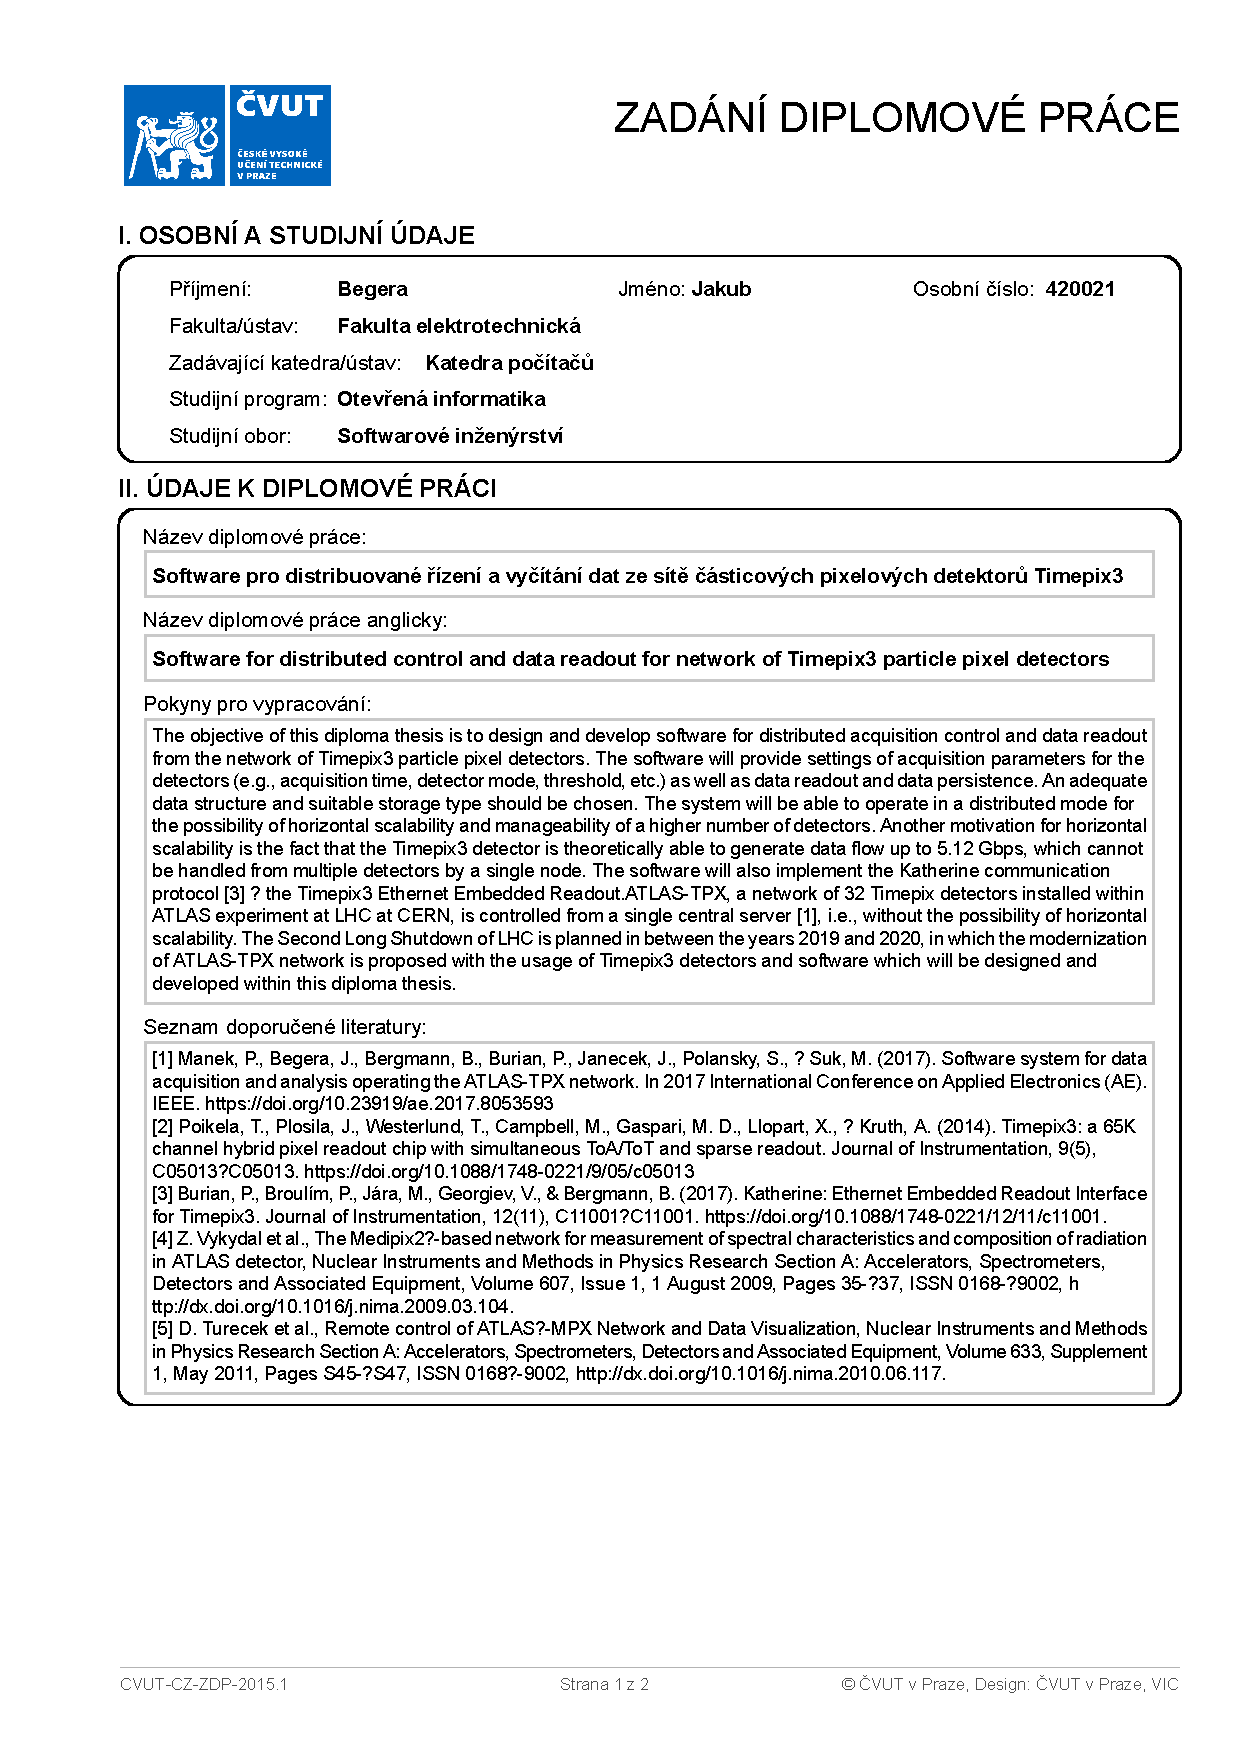
\includepdf[pages=1,pagecommand={},offset=0cm -3cm]{zadani.pdf}
	\includepdf[pages=2,pagecommand={},offset=0cm -3cm]{zadani.pdf}
	\newpage

	%%%%%%%%%%%%%%%%%%%%%%%%%%%    
	% Poděkovani / Acknowledgements 
	\acknowledgements
	\noindent
	\todo


	%%%%%%%%%%%%%%%%%%%%%%%%%%%   
	% Prohlášení / Declaration 

	\declaration{V~Praze dne 27.\,5.\,2016}


	%%%%%%%%%%%%%%%%%%%%%%%%%%%%    
	% Abstrakt / Abstract 
 
	\abstractpage

	\todo abstrakt anglicky

	
	\vglue60mm
	\noindent{\Huge \textbf{Abstrakt}}
	\vskip 2.75\baselineskip

	\todo abstrakt česky


	%%%%%%%%%%%%%%%%%%%%%%%%%%    
	% obsahy a~seznamy
	\tableofcontents		% Obsah
	\listoffigures			% Seznam obrázků
	\listoftables			% Seznam tabulek
	\listofcodes			% Seznam zdrojových kódů	

	%%%%%%%%%%%%%%%%%%%%%%%%%% 
	% začátek textu  
	\mainbodystarts

\addbibresource{reference.bib}

\chapter{Introduction}\label{chap01}
Test
\addbibresource{reference.bib}

\chapter{Úvod do hybridních částicových pixelových detektorů}\label{chap:detectors}
Ionizující záření je lidskými smysli nedetekovatelné, avšak jeho studie nám umožňuje pochopit podstatu hmoty, její vlastnosti a interakce. To lidstvu umožnilo mnohé aplikace, jako je například protonová terapie \cite{tpx_app_radiotherapy}, defektoskopie nebo zkoumání pravosti uměleckých děl. První pokusy o detekci ionizujícího záření sahají do počátku 20. století, kde pomocí mlžné komory se prvně podařilo zachytit trajektorii nabitých částic. Rozvoj polovodičové technologie dal vzniku novým detekčním technologiím až po v současné době nejpokrokovějším - pixelovým detektorům.

Existuje celá řada částicových pixelových detektorů, ale v této kapitole budou popsány jen hybridní pixelové detektory, pro které je typické, že se skládají ze dvou nezávisle vyrobených částí - senzoru a vyčítacího čipu. To oproti monolitickým detektorů, kde vyčítací elektronika je součástí senzoru přináší řadu výhod, jako například snížení výrobních nákladů nebo možnost kombinace vyčítacího čipu se senzory různých materiálů (\textit{Si}, \textit{GaAs}, \textit{CaTe} apod.) a tlouštěk (vetšinou $300\mu m$, nebo $500\mu m$).

Na tomto místě je třeba zmínit, že existuje více druhů těchto detektorů (\textit{AGH Fermilab, Pilatus, Philips Chromaix} apod.)\cite{detectors_review}, v této práci budou použity použity pouze detektory z rodiny detektorů Medipix.

%********************************************************************************
% Hardwarová architektura
%********************************************************************************
\section{Hardwarová architektura}
\begin{figure}[th]
	\begin{center}
		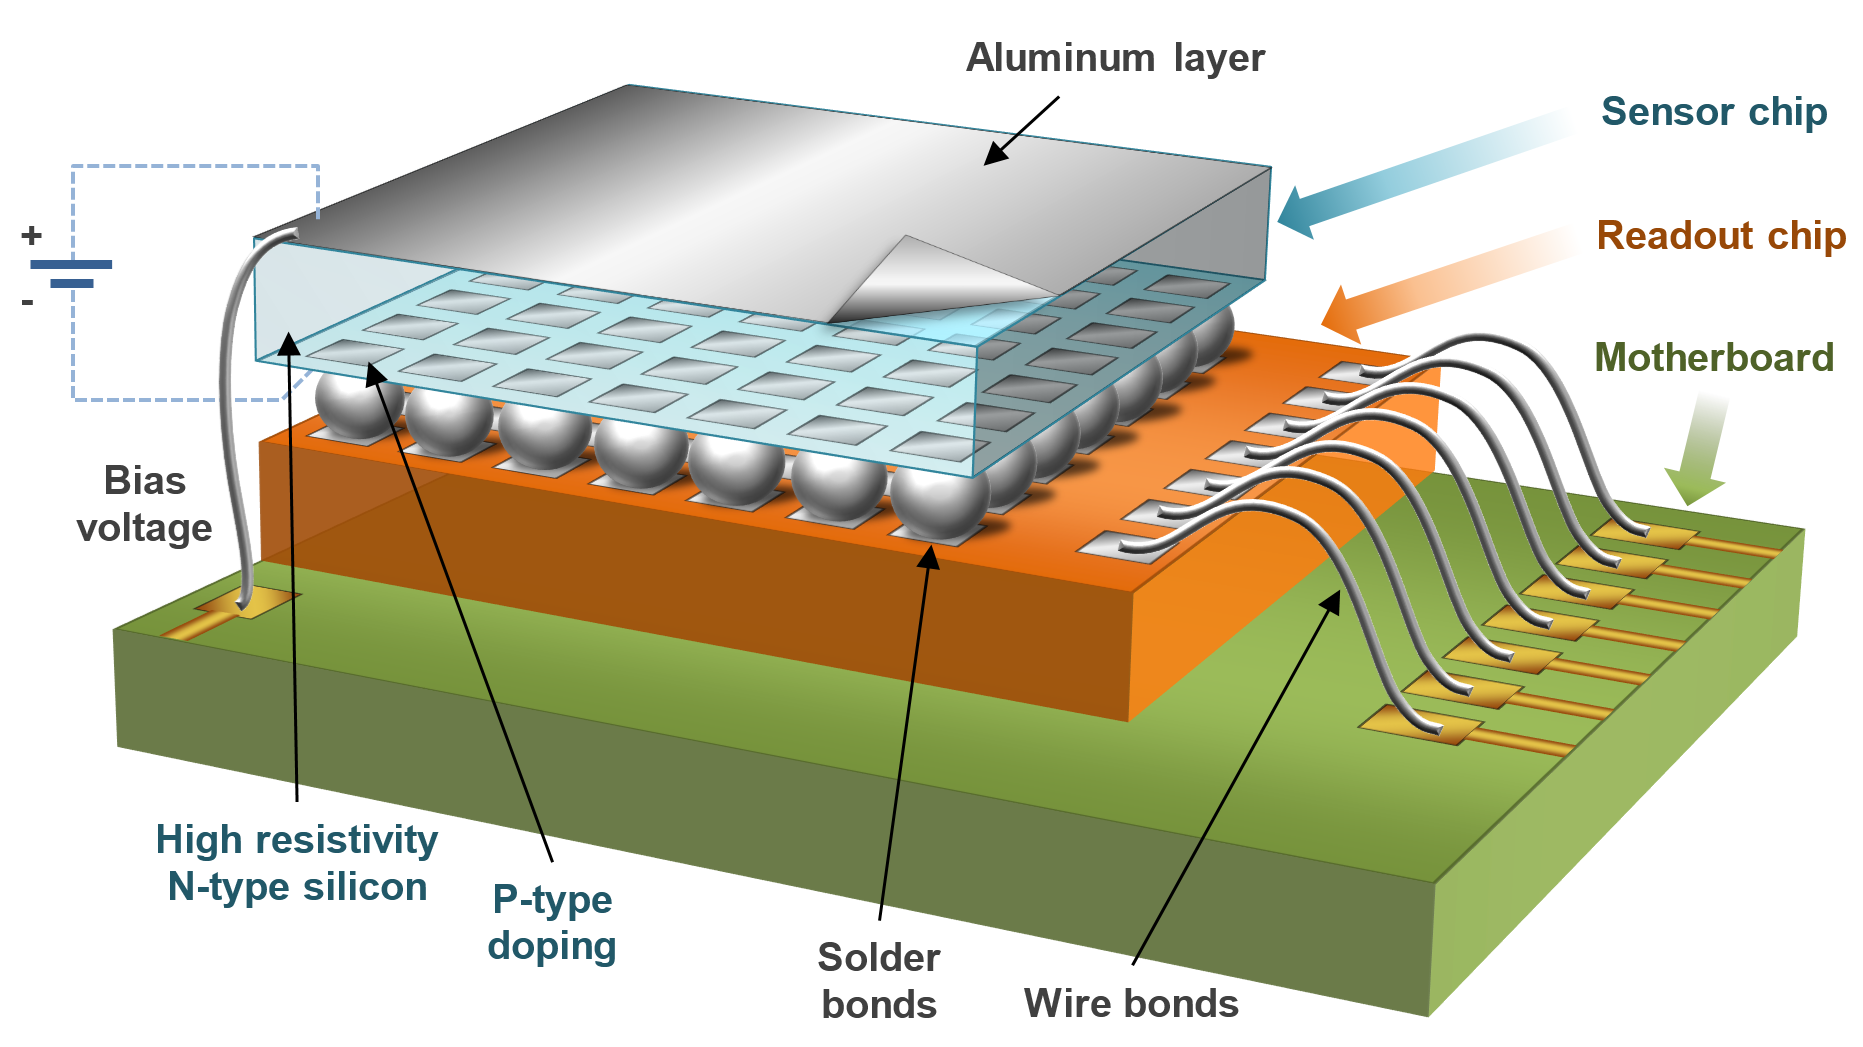
\includegraphics[width=12cm]{figures/det_chip.png}
		\caption{Struktura hybridního polovodičového pixelového detektoru Timepix3, skládající se z vyčítacího čipu a polovodičového senzoru \cite{PlatkevicDisertace}.}
		\label{fig:det:chip}
	\end{center}
\end{figure}
Většina hybridních částicových pixelových detektorů rodiny Medipix obsahuje matici $256\times256$ pixelů. Každý z nich má stanu o délce $55~\mu m$, takže senzor čítající $65536$ má plochu $1.4 \times 1.4 cm^2$. 

Na obrázku \ref{fig:det:chip} je znázorněna struktura detektoru Timepix3. Vrchní část detektoru tvoří polovodičový senzor, který je nejčastěji vyroben z křemíku, ale výjimkou není také \textit{GaAs} nebo \textit{CaTe}. Jednotlivé pixely senzoru jsou spojeny s integrovaným \texttt{ASIC}\footnote{z angl. Application Specific Integrated Circuit} vyčítacím čipem pomocí technologie zvané \textit{Bump-Bounding}. Vyčítací čip je pak propojen se základní deskou pomocí \textit{wire-bound}, z které je ještě přivedeno měřící napětí na senzor detektoru (tzv. \textit{bias}).


%********************************************************************************
% Princip detekce
%********************************************************************************
\section{Princip detekce}\label{chap:detectors:princip}
\begin{figure}[th]
	\begin{center}
		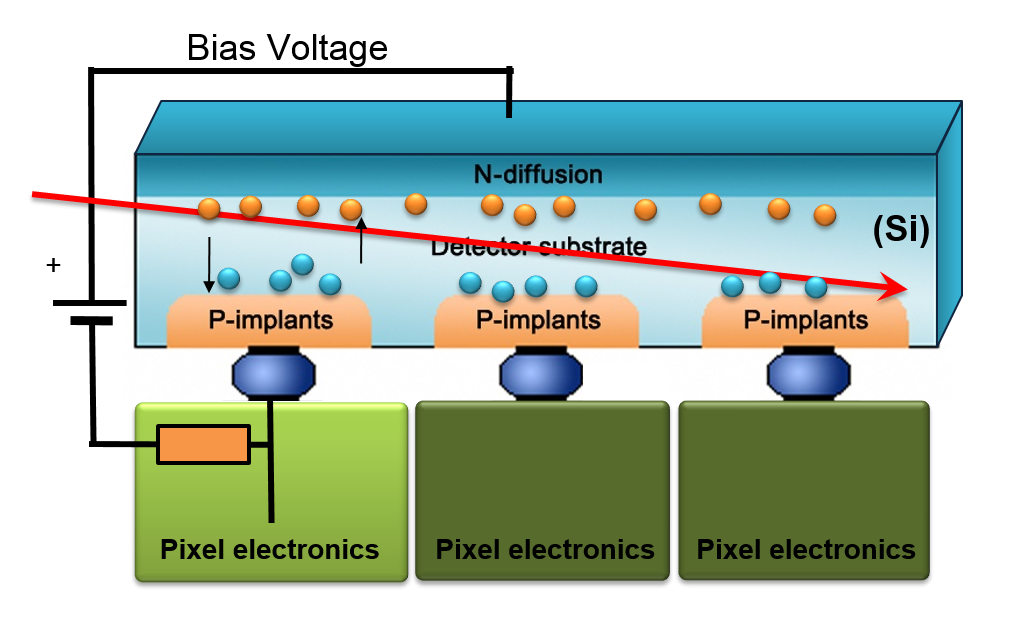
\includegraphics[width=10cm]{figures/det_recombination.png}
		\caption{Princip detekce ionizujícího záření detektorem Timepix3 \cite{PlatkevicDisertace}.}
		\label{fig:det:recombination}
	\end{center}
\end{figure}

Princip detekce ionizujícího záření pixelovými detektory je založen na známém jevu detekce ionizujícího záření v polovodiči. 

Jako náhradní schéma jednoho pixelu si lze představit diodu zapojenou v závěrném směru, kterou bez přítomnosti ionizujícího záření protéká minimální proud. Vnikne-li do senzoru ionizující částice a dojde k její interakci se senzorem, resp. část její energie je deponována do polovodičového objemu senzoru, dojde v senzoru ke vzniku elektron-děrových páru a díky lavinovému efektu i k následnému otevření PN přechodu (viz. na obr. \ref{fig:det:recombination}, kde červená šipka znázorňuje interagující částici, elektrony jsou znázorněny žlutě, modře díry).

Vzniklý proudový impulz je měřícím odporem převeden na napětí, které je komparátorem porovnáno s prahovým napětím (tzv. \textit{threshold}). Výsledek této komparace je dále CMOS obvodem zpracován, dle použitého měřícího módu, jak bude ukázáno v kapitole \ref{chap:detectors:operation_modes}.

Na rozdíl od CCD technologii, CMOS readout \textit{Timepix}/\textit{Medipix} detektorů negeneruje temný proud\footnote{Termín charakterizující vyčítací šum u CCD snímačů. Obvykle je udáván v elektronech za sekundu při konstantní teplotě a ve tmě.}, díky odstínění signálu od šumu pomocí komparačního napětí. To znamená, že doba jedné akvizice je teoreticky neomezena, protože detektor je schopný detekovat jen ty částice, jejíchž deponovaná energie (resp. amplituda vzniklého napěťového pulzu) je větší, než \textit{threshold}.

%********************************************************************************
% Operační módy detektoru
%********************************************************************************
\section{Operační módy detektoru}\label{chap:detectors:operation_modes}
\begin{figure}[th]
	\begin{center}
		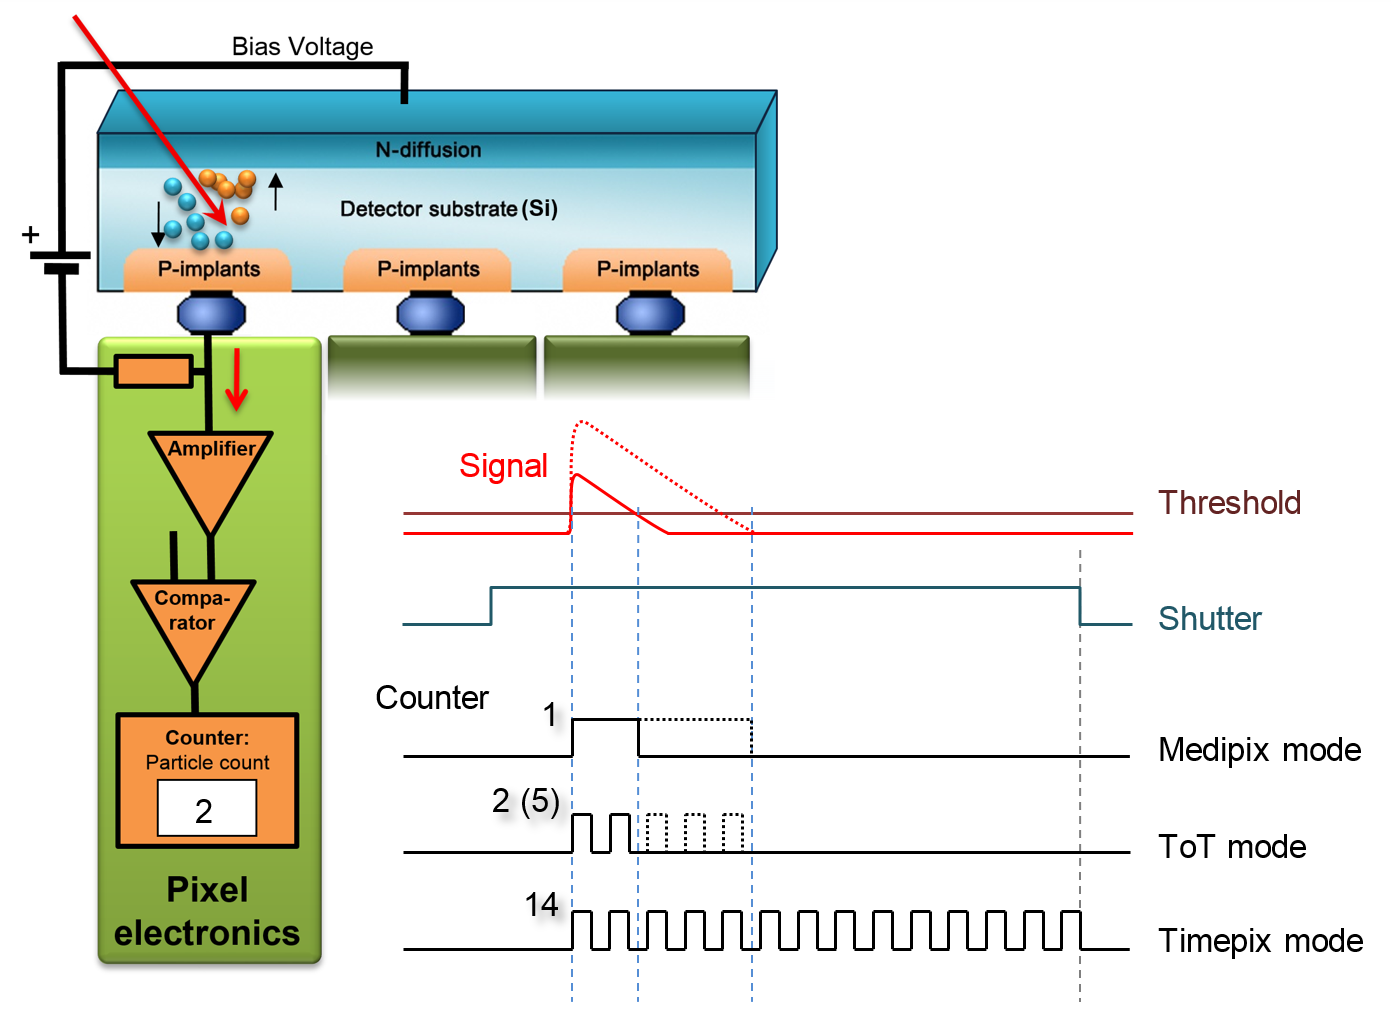
\includegraphics[width=14cm]{figures/det_pix.png}
		\caption{Zpracování signálu pixelem detektoru dle nastaveného módu (\textit{Medipix}, \textit{ToT} a \textit{ToA}) \cite{PlatkevicDisertace}.}
		\label{fig:det:modes}
	\end{center}
\end{figure}


V této podkapitole bude vysvětlena většina operačních módu, ve kterých detektory rodiny \textit{Medipix} jsou schopny pracovat. 

Jak už bylo popsáno v předchozí kapitole, interagovaná částice vyvolá napěťový impulz, jehož tvar koreluje s deponovanou energií. Pro účely analýzy se ale používá pouze binární informace o překročení prahového napětí v čase. Výsledek této analýzy je po jejím dokončení uložen ve 14-bitovém registru pixelu.

Na obr. \ref{chap:detectors:operation_modes} je znázorněn příklad zpracování analýzy signálu následujícími módy:
\begin{description}
    \item[Medipix mód (Counting mód)] V tomto módu je čítač inkrementován v každém cyklu měřící frekvence, pokud měřící napětí překročilo prahové napětí pixelu. Na konci akvizice pak hodnota čítače odpovídá počtu zaznamenaných částic.
    \item[Time-Over-Threshold (ToT)] Pracuje-li pixel v tomto módu, pak jeho čítač je inkrementování v každém cyklu měřící frekvence, pokud měřící napětí je vyšší, než prahové napětí pixelu. Hodnota uložená v čítači odpovídá deponované energii interagovaných částic. Mezi energií a \texttt{ToT} je nelineární závislost a její zkoumání je předmětem energetické kalibrace detektoru, jak bude ukázáno v kapitole \ref{chap:detectors:calibration:energy}. Tento mód má široké spektrum aplikací, například \cite{tot_app_counting} nebo \cite{tpx_app_radiotherapy}.
    \item[Time-of-Arrival (ToA)] Tímto módem disponují pouze detektory \textit{Timepix} a \textit{Timepix3}, avšak nesdílí stejný princip. Zatímco \textit{Timepix} detektor začne inkrementovat čítač v každém cyklu měřící frekvence po první náběžné hraně z komparátoru, \textit{Timepix3} na náběžnou hranu uloží do 14-bitového registru aktuální časové razítko z hodin detektoru. V obou případech \texttt{ToA} udává čas první interakce částice v dané akvizici.
\end{description}

%********************************************************************************
% Vyčítání naměřených dat
%********************************************************************************
\section{Vyčítání naměřených dat}\label{chap:detectors:readout}
Jednotlivé detektory rodiny \textit{Medipix} mají různou hardwarovou podporu pro vyčítání naměřených dat. Detektory vždy podporují alespoň jeden z těchto módů:
\begin{description}
	\item[Frame-Based] Pracuje-li detektor v tomto módu, pak jsou všechny registry čítačů pixelů vyčítány najednou, po dokončení aktuálního snímku. Vždy je třeba vyčíst všechny pixely bez ohledu na naměřenou hodnotu.
	\item[Data-Driven] Tento mód, také označovaný jako \textit{Event-Driven}, byl prvně použit v detektoru \textit{Timepix3}. Pracuje-li detektor v tomto módu, pak v průběhu akvizice dat (resp. když \textit{shutter} signál na nastaven na úroveň \texttt{HIGH}) každý pixel po zpracování události notifikuje readout interface o tom, že nová data jsou připravena k vyčtení a readout interface je pak bez prodlení vyčte a dále zpracuje.
\end{description}

Na obrázku \ref{fig:det:frame_vs_event_driven} je vidět hlavní motivace pro zavedení podpory \textit{Data-Driven} módu u detektoru \textit{Timepix3}. Ukázalo se, že \textit{Data-Driven} mód je efektivnější při takových měření, kde okupance snímků je menší než zhruba $50\%$. Po překročení této meze je efektivnější použití \textit{Frame-Based} módů, protože není třeba přenášet souřadnice zasažených pixelů. Podle \cite{timepix3} vyčítací čas může být definován následovně:
\begin{equation}\label{eq:det:readout_time}
	T_{readout} = N_{pixels}*bits_{pixel}/BW
\end{equation}
kde:
\begin{changemargin}{1.5cm}{1cm} 
	\begin{itemize}
		\item[$N_{pixels}$] je počet pixelů které je potřeba vyčíst (pro \textit{Frame-Based} mód jsou to všechny pixely detektoru ($256\times256$) a pro \textit{Data-Driven} je to počet zasažených pixelů),
		\item[$bits_{pixel}$] je počet bitů na pixel ($28 b$ v \textit{Frame-Based} módu a $28b + 16b$ v \textit{Data-Driven} módu kvůli nutnosti přenášení adresy pixelu) a
		\item[$BW$] je počet bytů za vteřinu, které je možné vyčíst z detektoru (\textit{bandwidth}). 
	\end{itemize}
\end{changemargin}

\begin{figure}[th]
	\begin{center}
		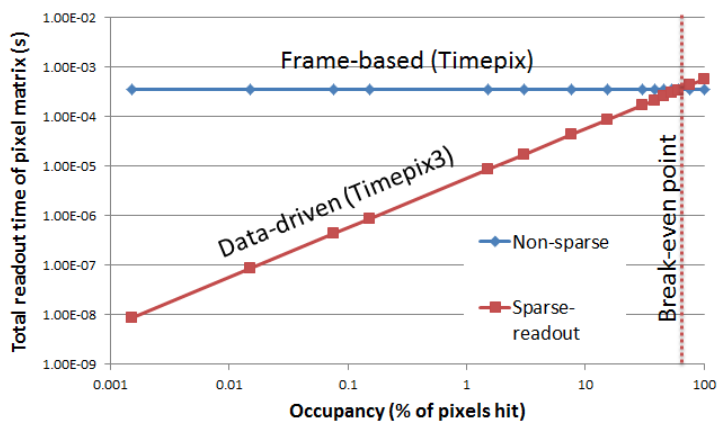
\includegraphics[width=14cm]{figures/det_frame_vs_event_driven.png}
		\caption{Doba vyčítání detektoru za použití \textit{Frame-based} (non-sparse) a \textit{Data-driven} (sparse) módu \cite{timepix3}.}
		\label{fig:det:frame_vs_event_driven}
	\end{center}
\end{figure}

%********************************************************************************
% Kalibrace
%********************************************************************************
\section{Kalibrace}\label{chap:detectors:calibration}
Každý detektor má své specifické vlastnosti, které jsou dány nejenom výrobním procesem, ale i závislostí na opotřebení a únavě materiálu v čase, okolní teplotě nebo na nastavených měřících parametrech (například \textit{bias}). Hlavní motivací pro kalibraci detektorů je minimalizace systematické chyby měření. Z pohledu aplikace získaných kalibračních dat je možné kalibrační metody rozdělit do dvou kategorií:
\begin{enumerate}[label=(\roman*)]
	\item Použití v průběhu akvizice dat - jedná se o data, která jsou použita pro nastavení akvizice dat v detektoru a mají přímý vliv na naměřená data, která danou metodou není možné dodatečně kalibrovat. Do této kategorie spadá například \textit{treshold equalizace} (viz \ref{chap:detectors:calibration:equalization}).
	\item Transformace naměřených dat - v tomto případě jsou kalibrační data aplikovaná dodatečně na naměřená data. Tento přístup má výhodu v možnosti dodatečné kalibrace již naměřených dat. To této kategorie spadá například \textit{Energetická kalibrace} (viz \ref{chap:detectors:calibration:energy}) nebo \textit{Time-Walk korekce} (viz \ref{chap:detectors:calibration:timeWalk}).
\end{enumerate}

\subsection{Treshold equalizace}\label{chap:detectors:calibration:equalization}
V podkapitole \ref{chap:detectors:princip} a \ref{chap:detectors:operation_modes} již bylo vysvětleno použití prahového napětí (\textit{treshold}) v průběhu akvizice dat detektorem. Každý pixel detektoru má ale rozdílné fyzikální vlastnosti dané výrobním procesem, s čímž souvisí i citlivost (resp. oddělení užitečného signálu od šumu) jednotlivých pixelů. Kromě globální hodnoty tresholdu je možné pro každý pixel upravit citlivost pomocí lokální $4b$ hodnoty tresholdu (viz obr. \ref{fig:det:medipix_overview:timepix3_schema}).

Vlastní proces equalizace probíhá tak, že se udělá treshold scan přes všechny hodnoty, přičemž je třeba minimalizovat interakce detektoru z částicemi. V běžné praxi stačí detektor dostatečně odstínit. Výstupem tohoto procesu je pak globální treshold a jeho 4-bitové korekce pro jednotlivé pixely.

Jako vedlejší produkt tohoto procesu je rovněž maskovací matice detektoru, které obsahuje šumějící, nebo jinak poškozené pixely. To jsou například takové pixely, které bez přítomnosti interagujících částic hlásí překročení tresholdu.

\subsection{Energetická kalibrace}\label{chap:detectors:calibration:energy}
\begin{figure}[th]
	\begin{center}
		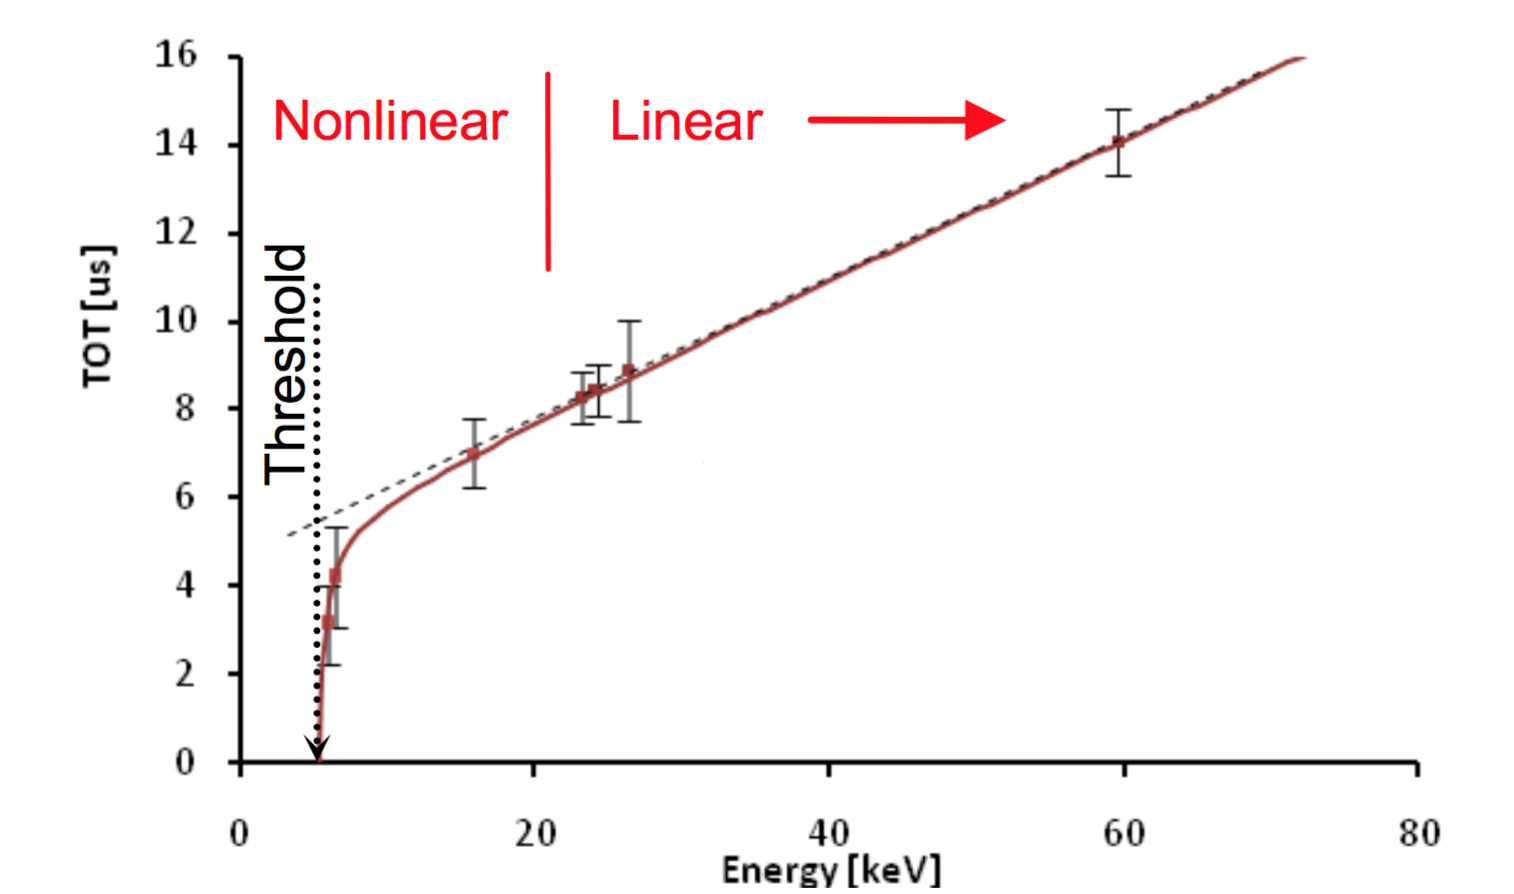
\includegraphics[width=13cm]{figures/calib_function.png}
		\caption{Kalibrační funkce, udávající závislost mezi energií v \texttt{keV} a \texttt{ToT} \cite{Jakubek2011S262}, vzniklá proložením získaných kalibračních bodů funkcí \ref{eq:det:energyCalib} a sestávající se ze dvou částí - (i) nelineární částí pro oblast nižších energií (hyperbola) a (ii) lineární částí pro vyšší energie (přijímka).}
		\label{fig:det:calib:calib_function}
	\end{center}
\end{figure}

V předchozí části práce byl již představen \textit{Time-Over-Treshold} mód (viz \ref{chap:detectors:operation_modes}), ve kterém je detektor schopný měřit deponovanou energii interagovaných v částic, která je udávána v \texttt{ToT}. Jak již bylo ukázáno, vztah mezi energií v \textit{keV} a \texttt{ToT} je nelineární závislost a závisí na fyzikální vlastnostech daného pixelu, což je předmětem energetické kalibrace, která bude v této podkapitole popsána.

Tato metoda \cite{Jakubek2011S262} spočívá v provedení několika sad měření se zdroji ionizujícího záření, jejichž energie jsou předem známy, a v jejich analytickém zpracování a vytvoření kalibrační funkce \ref{eq:det:energyCalib} pro každý pixel detektoru. V předchozí práci \cite{BegeraBcThesis2016} byly tyto metody podrobně popsány a byl vytvořen software, který uživateli umožňuje vytvoření energetické kalibrace detektoru z naměřených dat.

\begin{equation}\label{eq:det:energyCalib}
	f_{calib}(x) = ax + b - \frac{c}{x-t}
\end{equation}

Pro měření kalibračních dat se jako efektivní řešení v praxi ukázalo použití rentgenové fluorescence\footnote{Děj ke kterému dochází při ozařování materiálu (nejčastěji \textit{Cu}, \textit{Fe}, \text{In} apod.) rentgenovým zářením, při kterém jsou z něj vyráženy excitované elektrony. Při vyražení elektronu na nižší energetické úrovni, elektron z vyšší energetické úrovně obsadí jeho místo a přebytečnou energii emituje formou vyzářeného fotonu - fluorescenčního záření, jehož charakteristické monoenergetické spektrum je pro většinu prvků dobře známé.} \cite{Jakubek-radiography_and_charge_sharing}. Pro zajištění dobré kvality kalibrace je třeba naměřit takový počet událostí, aby spektra ve snímcích byla dobře rozeznatelná. Z naměřených dat jsou vyfiltrovány pouze tzv. \textit{Single-hit} události\footnote{Události, ve kterých částice interagovala pouze s jedním pixelem detektoru}, aby se minimalizovaly negativní vlastnosti \textit{Charge-sharing} efektu (díky společné elektrodě senzoru jsou díky interagující částici vzniklé elektrony zpracovány více pixely najednou a část deponované energie nemusí být ASIC čipem zpracována, protože vzniklý signál může být nižší než treshold daného pixelu).

\begin{figure}[th]
	\begin{center}
		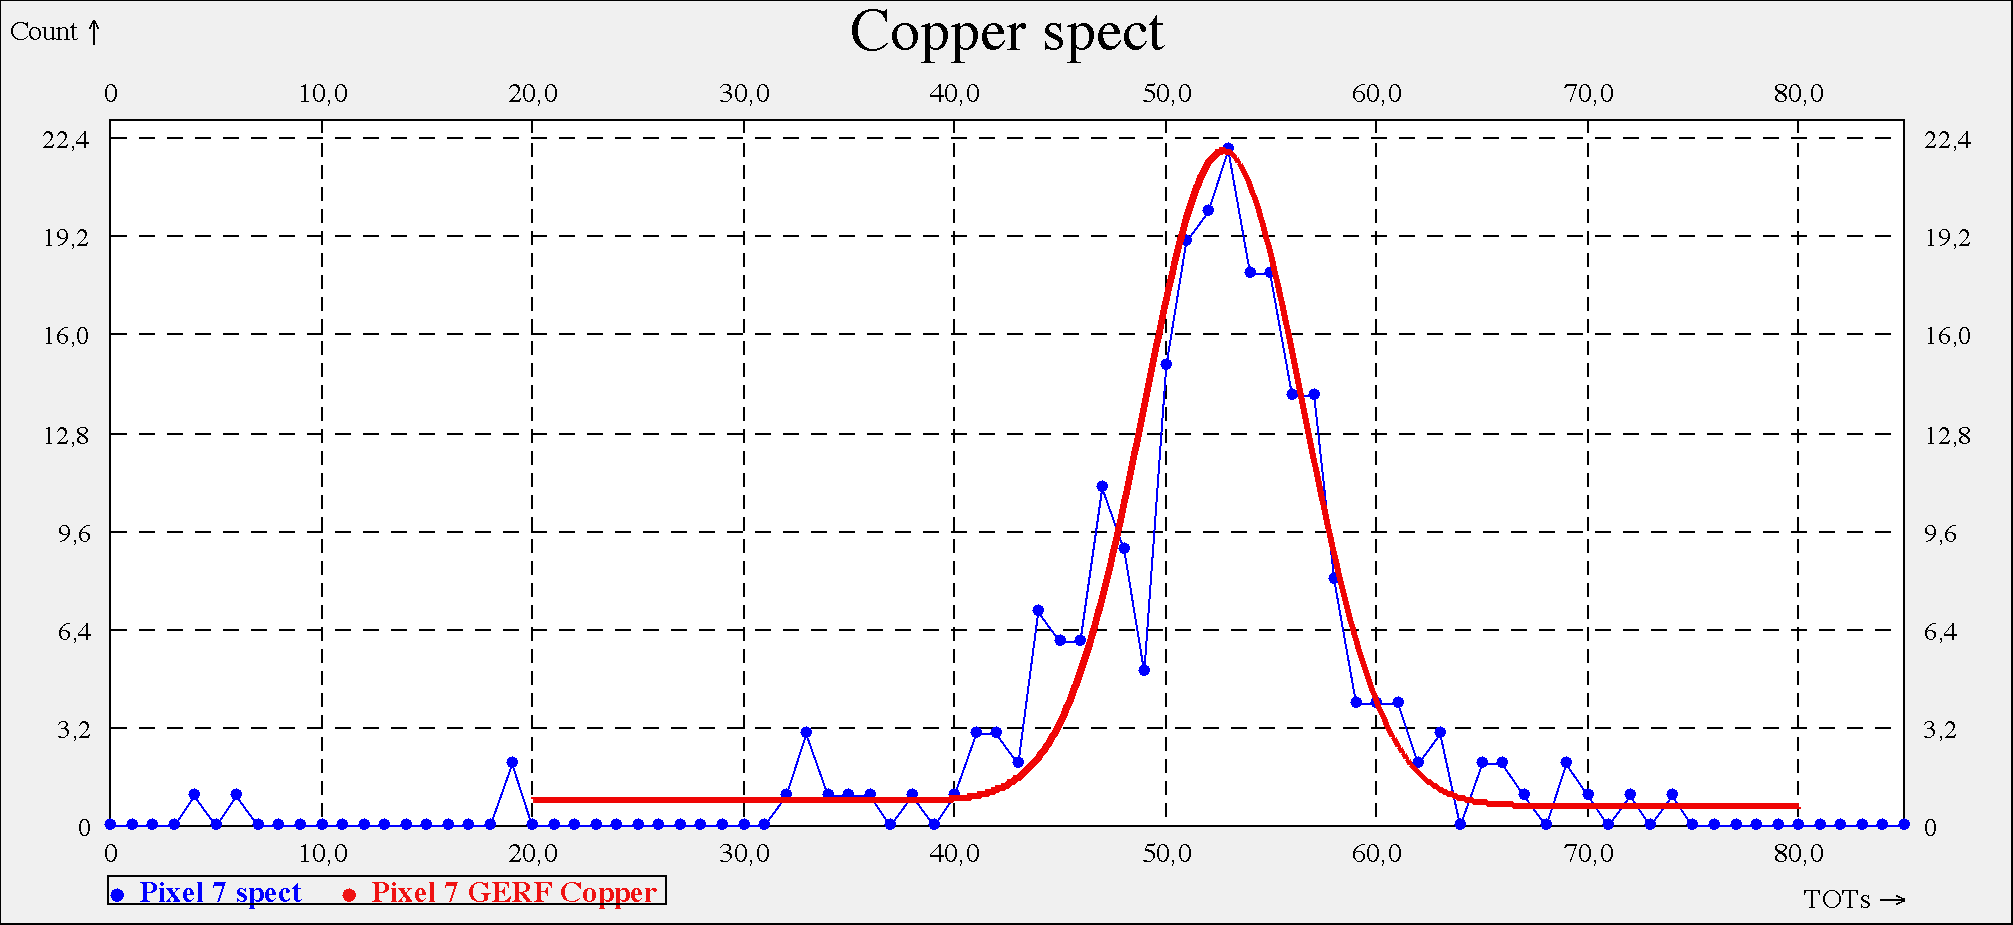
\includegraphics[width=15cm]{figures/calib_gerf.png}
		\caption{Příklad energetického spektra jednoho pixelu Timepix detektoru s proloženou funkcí \ref{eq:det:gerf} \cite{BegeraBcThesis2016}.}
		\label{fig:det:calib:gerf}
	\end{center}
\end{figure}

Z jednotlivých měření jsou pro každý pixel detektoru vytvořena spektra \texttt{ToT} hodnot. Na obrázku \ref{fig:det:calib:gerf} je znázorněn příklad takového spektra, získaného z fluorescence mědi. Požadovaný kalibrační bod se získá střední hodnoty \texttt{ToT} a tabulkové hodnoty energie fluorescenčního záření mědi. Střední hodnota je získána proložením spektra funkcí \ref{eq:det:gerf} - jedná se o součet Gaussovy funkce a Gaussovy chybové funkce (kvůli levé nesymetrii vzniklé \textit{Charge-sharing} efektem)
\begin{equation}\label{eq:det:gerf}
	f_{GERF}(x) = \underbrace{Ae^{ -\frac{(x-\mu)^2}{2\sigma^2} }}_{\text{Gaussova funkce}} +
	\underbrace{ \frac{avg_{right} - avg_{left}}{\sigma\sqrt{2\pi}} \int_{-\infty}^t e^{ -\frac{(t-\mu)^2}{2\sigma^2} } + avg_{left}}_{\text{Gaussova chybová funkce}},
\end{equation}
kde:
\begin{changemargin}{1.5cm}{1cm} 
	\begin{itemize}
		\item [$A$] je amplituda,
		\item [$\mu$] je stření hodnota hledané energie,
		\item [$\sigma$] je rozptyl střední hodnoty energie $\mu$, který je možné vypočítat ze vzorce 
			\ref{eq:det:gerf_sigma}, kde \texttt{FWHM}\footnote{z angl. Full Width at Half Maximum} udává šířku gausiánu v~polovině jeho výšky a
		\item [$avg_{right}$, $avg_{left}$] je průměrná hodnota spektra na pravém (resp. levém) úpatí gausiánu.
	\end{itemize}
\end{changemargin}

\begin{equation}\label{eq:det:gerf_sigma}
	\sigma = \frac{2\sqrt{2ln_2}}{FWHM}
\end{equation}

\subsection{Time-Walk korekce}\label{chap:detectors:calibration:timeWalk}

\textit{Time-Walk} efekt je nežádoucí jev, který vzniká při interakci ionizujícího záření o různé energii. Velikost deponované energie má vliv na amplitudu a sklon napěťového pulzu na zesilovači pixelu. Při interakci ionizující částice s více pixely je pak díky tomuto jevu interagovanými pixely zaznamenána jiná hodnota \textit{Time-of-Arrival} (ToA), i přes to že událost byla způsobena stejnou částicí a ToA by měl být stejný. Viz obrázek \ref{fig:det:calib:timeWalk}, kde jsou pro interakci stejné částice čtyřmi sousedními pixely zaznamenány různé hodnoty ToA. 

\begin{figure}
	\begin{center}
		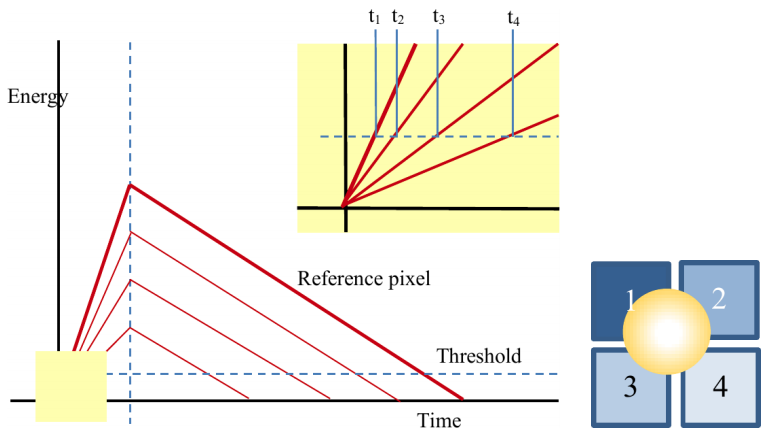
\includegraphics[width=12cm]{figures/calib_timeWalk.png}
		\caption{\textit{Time-walk} efekt: příklad interakce jedné částice se čtyřmi pixely detektoru, kde v každém pixelu byla deponována jiná energie, což na výstupů zesilovačů pixelů způsobilo jiné hodnoty napětí. Díky rozdílné charakteristice náběžné hrany pulzů byl treshold překročen v různých časech ($t_{1-4}$) \cite{Turecek2016TimeWakl}.}
		\label{fig:det:calib:timeWalk}
	\end{center}
\end{figure}

S použitím detektoru \textit{Timepix3}\cite{timepix3} je možné tuto energeticky závislou chybu eliminovat za použití kalibrační metody \cite{Turecek2016TimeWakl}, protože tento detektor umožňuje měřit v ToA a ToT módu současně. Tato kalibrační metoda spočívá v analytickém zpracování dat získaných z měření se zdrojem alfa částic (v \cite{Turecek2016TimeWakl} použito $^{241}$\texttt{Am}), které generuje clustery o velikosti maximálně čtyři pixely. Nejprve je však třeba potřeba energeticky zkalibrovat \ref{chap:detectors:calibration:energy}. 

O vybraných clusterech o velikosti 3 a 4 pixely pro $^{241}$\texttt{Am} víme, že součet jejich energií je $59.5keV$. Z clusteru je vybraný pixel s energií $30keV$, který je použit jako referenční (na \ref{chap:detectors:calibration:timeWalk} jako $t_1$), zbylá energie je náhodně rozdělena mezi ostatní pixely (na \ref{chap:detectors:calibration:timeWalk} jako $t_{2-4}$). Jednotlivé rozdíly $t_i+t_1$ jsou analytickými metodami, popsanými v \cite{Turecek2016TimeWakl}, zpracovány a výsledkem tohoto procesu jsou konstanty $c,d$ pro každý pixel detektoru, kterými lze vypočítat jeho \textit{Time-Walk offset} $\Delta T$:

\begin{equation}\label{eq:det:timeWalk}
	\Delta T = \frac{c}{(E - E_0)^d}
\end{equation}
kde:
\begin{changemargin}{1.5cm}{1cm} 
	\begin{itemize}
		\item [$\Delta T$] je \textit{Time-Walk} korekce pixelu [$ns$] (výsledná hodnota ToA je pak rovna $ToA-\Delta T$),
		\item [$E$] je energie pixelu [keV],
		\item [$E_0$] je treshold pixelu [keV] a
		\item [$c,d$] jsou konstanty.
	\end{itemize}
\end{changemargin}

\subsection{ToA offset korekce}\label{chap:detectors:calibration:toa_correction}
Jedná se o jev, ke kterému dochází u \textit{Timepix3} detektorů z důvodu chyby hardware, který způsobuje špatnou synchronizaci časového razítka napříč sloupci detektoru \cite{Katherine}. Tato chyba vzniká jen při zapnutí detektoru a poté je \texttt{ToA} offset již stabilní, takže je možné vytvořit korekci.

Odstranění tohoto jevu spočívá ve vytvoření kompenzační tabulku pomocí středních hodnot interních testovacích pulzů \cite{timepix3}. Pro získání správných hodnot \texttt{ToA} z naměřených dat stačí jen odečíst příslušnou hodnotu z korekční tabulky.

%********************************************************************************
% Přehled detektorů rodiny Medipix
%********************************************************************************
\section{Přehled detektorů rodiny Medipix}\label{chap:detectors:medipix_overview}
V této podkapitole budou stručně představeny jednotlivé detektory, které byly vyvinuty v rámci Medipix kolaborace \cite{medipix-www}.

\begin{figure}
	\begin{center}
		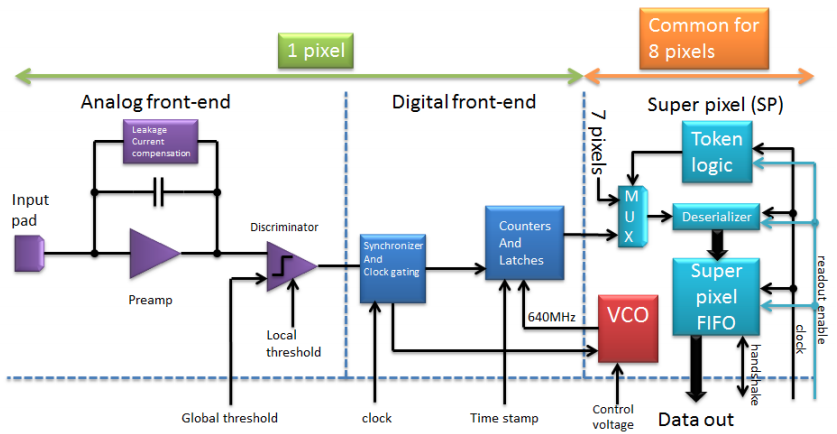
\includegraphics[width=15cm]{figures/det_timepix3_schema.png}
		\caption{Schéma pixelu detektoru \textit{Timepix3} se společnou elektronikou pro 8 pixelů (tzv.\textit{Super-pixel}) \cite{timepix3}.}
		\label{fig:det:medipix_overview:timepix3_schema}
	\end{center}
\end{figure}

\begin{description}

	\item[Medipix1] V roce 1998 byl vyvinut detektor \textit{Medipix1} \cite{medipix1}, také zvaný \textit{Photon-Counting-Chip}, byl první velkoplošný detektor používající CMOS technologie. S maticí $64\times64$ pixelů, každým o hraně $170~\mu m$, má celkovou aktivní plochu $1,1~cm^2$. I přes malý počet pixelů a jejich velkou rozteč, tento detektor prokázal dobré rozlišovací vlastnosti, především pak v rentgenovém zobrazování. 
	
	Detektor je vyrobený pomocí $1~\mu m$ technologie a je schopný operovat pouze v Medipix módu (viz \ref{fig:det:modes}) a podporuje pouze vyčítání po snímcích (viz \ref{chap:detectors:readout}).
	
	\item[Medipix2] V roce 2001 byl vyvinut detektor \textit{Medipix2} \cite{medipix2}, jako náhrada za svého předchůdce \textit{Medipix1}. Díky $250~nm$ technologii bylo možné zvýšit počet pixelů a zároveň snížit jejich rozteč - detektor má $256\times256$ pixelů, každý o hraně $55~\mu m$. Navíc má dva tresholdy s diskriminací na 4 pixely. 
	
	Stejně jako svůj předchůdce je schopný operovat pouze v Medipix módu (viz \ref{fig:det:modes}) a podporuje pouze vyčítání po snímcích (viz \ref{chap:detectors:readout}).
	
	\item[Timepix]\label{chap:detectors:medipix_overview:timepix} V roce 2006 byl vyvinut detektor \textit{Timepix} \cite{timepix}, který vychází z detektoru \textit{Medipix2}. Detektory mají stejné rozměry, ale architektura pixelů se změnila. Nově každý pixel detektoru umožňuje nezávisle měřit čas interakce částice, její energii, nebo je schopný počítat jednotlivé interakce. 
	
	Detektor je schopný operovat v \texttt{ToT}, \texttt{ToA}, nebo v Medipix módu (viz \ref{fig:det:modes}) a podporuje pouze vyčítání po snímcích (viz \ref{chap:detectors:readout}).
	
	\item[Medipix3] V roce 2011 byl vyvinut detektor \textit{Medipix3} \cite{medipix3}, jako nástupce \textit{Medipix2} detektoru. Rozměry detektoru zůstaly zachovány ($256\times256$ pixelů, každý o hraně $55~\mu m$), ale díky $130~nm$ technologii byla funkce jednotlivých pixelů vylepšena. Detektor nově umožňuje zvýšení energetického rozlišení díky potlačení \textit{Charge-Sharing} efektu (viz \ref{chap:detectors:calibration:energy}) pomocí integraci náboje do clusteru $4\times4$ pixelů. 
	
	Každý pixel má dva 14-bitové čítače. Jednotlivé pixely můžou být naprogramovány tak, aby vždy měřily za pomocí jednoho čítače, zatímco je hodnota z druhého čítače vyčítána, což umožňuje měření bez mrtvé doby.

	Také je možné zapojit tento readout čip (s pixelem o hraně $55~\mu m$) na senzor s pixely o hraně $110~\mu m$, takže výsledný super-pixel má k dispozici 8 čítačů a pomocí různých úrovní tresholdů jej lze použít jako 8-kanálový spektrometr.

	Stejně jako svůj předchůdce je schopný operovat pouze v Medipix módu (viz \ref{fig:det:modes}) a podporuje pouze vyčítání po snímcích (viz \ref{chap:detectors:readout}).

	\item[Timepix3]\label{chap:detectors:medipix_overview:timepix3} V roce 2014 byl vyvinut detektor \textit{Timepix3} \cite{timepix3}, jako nástupce \textit{Timepix} detektoru. Rozměry byly zachovány, ale bylo použita $130~\mu m$ výrobní technologie, jako u \textit{Medipix3}. Detektor nově umožňuje měřit v \texttt{ToA} a \texttt{ToT} současně a jeho časové rozlišení bylo vylepšeno více než na šestinásobek.

	Detektor nově umožňuje kromě vyčítání po snímcích i \textit{Data-Driven} mód, kde jsou data v rámci akvizice kontinuálně z detektoru vyčítána (viz \ref{chap:detectors:readout}). Takto navržená architektura umožňuje vyčítat data až do $40M_{hits}*cm^{-2}*s^{-1}$ bez globální mrtvé doby detektoru (pouze s lokální mrtvou dobou - pro jednotlivé pixely, ze kterých jsou vyčítána naměřená data).

	Na obrázku \ref{fig:det:medipix_overview:timepix3_schema} je znázorněno blokové schéma jednoho pixelu \textit{Timepix3} detektoru, který se skládá z analogové a digitální části (pro popis funkcionality viz \ref{chap:detectors:princip}). Na obrázku vpravo je pak společná elektronika, sdílená vždy 8 sousedními pixely (tzv.\textit{Super-pixel}).

\end{description}

%********************************************************************************
% Vyčítací rozhraní
%********************************************************************************
\section{Vyčítací rozhraní}\label{chap:detectors:readouts}
V této podkapitole bude popsáno několik vyčítacích rozhraní, které byly vyvinuty (v rámci \textit{Medipix kolaborace}\footnoteUrl{https://medipix.web.cern.ch}) ÚTEF ČVUT v Praze a jeho spinoff společností ADVACAM s.r.o. Pro komunikaci s \textit{Timepix3} detektorem bude v rámci této práce bude použito nově vyvinuté vyčítací rozhraní \textbf{Katherine} \cite{Katherine} \ref{chap:detectors:readouts:katherine}.

\subsection{FITPix}
FITPix \cite{fitpix} vyčítací rozhraní bylo vyvinuto v roce 2010 a skládá ze z programovatelného hradlového pole (\texttt{FPGA})\footnote{Z angl. Field Programmable Gate Array}, USB 2.0 rozhraní, DAC\footnote{Převodník digitálního signálu na analogový.} a ADC\footnote{Převodník analogového signálu na digitální.} převodníků a obvodů pro generování měřícího napětí (\textit{bias}).

Zařízení je s detektorem propojeno pomocí \textit{LVDS}\footnote{Z angl. Low-voltage differential signaling} a je schopné jeho plnohodnotného řízení, vč. nastavování hodnot (měřící frekvence, treshold, bias apod.), řízení akvizice a vyčítání naměřených dat rychlostí až $90$ snímků za sekundu. Zařízení rovněž umožňuje připojení externího trigger signálů pro synchronizované měření s více detektory současně.

FITPix je možné použít pouze jako nízkoúrovňové vyčítací rozhraní a veškerá business logika musí být implementována v připojeném počítači (na př. deserializace a derandomizace naměřených dat apod.). Jako řídící software je použit \textit{Pixelman}\cite{pixelman}. Zařízení je kompatibilní se všemi detektory uvedenými v \ref{chap:detectors:medipix_overview}, kromě \textit{Timepix3}.

\subsection{AdvaDAQ}
AdvaDAQ \cite{Turecek2016TimeWakl} je nástupcem vyčítacího rozhraní FITPix a kompatibilní se všemi detektory uvedenými v \ref{chap:detectors:medipix_overview}. Principem funkce vychází ze svého předchůdce, ale díky použitému rozhraní USB 3.0 je schopné dosahovat maximálního datového toku $2,9~Gb/s$. Deserializace naměřených dat byla implementována do firmware \textit{FPGA}. Pro řízení tohoto rozhraní, vizualizaci a analýzu naměřených dat byl vyvinut software Pixet.

\subsection{ATLAS Pix}\label{chap:detectors:readouts:atlaspix}
ATLAS Pix \cite{atlastpx_sw, BegeraBcThesis2016} je zařízení vyvinuté v rámci experimentu \textit{ATLAS-TPX}, síti 16 hybridních částicových detektorů \textit{Timepix}, instalované v rámci experimentu \textit{ATLAS} na \textit{LHC} v \textit{CERN}, operující od roku 2014.

Zařízení vzniklo modifikací vyčítacího rozhraní \textit{FITPix} a disponuje \texttt{FPGA}, \texttt{LVDS} zesilovačem a počítače \textit{Raspberry Pi}, ve kterém je implementován software, poskytující API pro své vzdálené řízení přes \texttt{TPC} protokol. Komunikace mezi \texttt{FPGA} a počítačem je realizována pomocí \texttt{SPI}\footnote{Z angl. Serial Peripheral Interface.} protokolu.

\subsection{Katherine}\label{chap:detectors:readouts:katherine}
\begin{figure}
	\begin{center}
		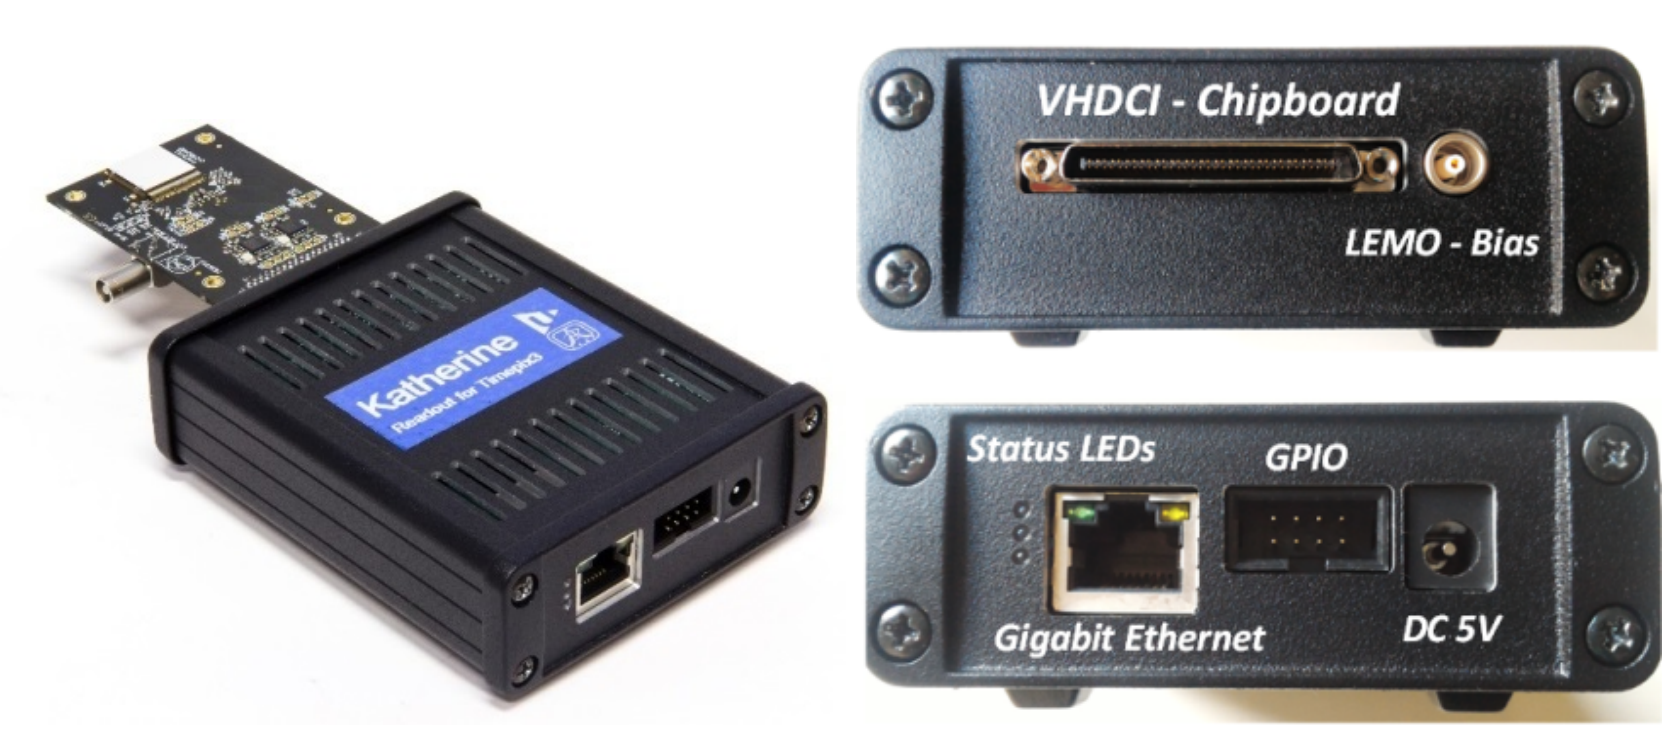
\includegraphics[width=15cm]{figures/det_katherine.png}
		\caption{Vyčítací rozhraní \textit{Katherine} s přípojeným detektorem \textit{Timepix3} vlevo a popisem vstupných a výstupních portů vpravo\cite{Katherine}.}
		\label{fig:det:readout:katherine}
	\end{center}
\end{figure}

Katherine \cite{Katherine} je pokročilé vyčítací rozhraní dedikované pro řízení jednoho \textit{Timepix3} detektoru, které v sobě obsahuje embedovaný počítač, čímž se vymezuje od ostatních vyčítacích rozhraní bez procesoru, kde business logika musí být implementována v připojeném počítači, což má negativní dopad na vytížení jeho procesoru. 

Hlavním benefitem zařízení je možnost jeho použití na experimentech, kde je nutná větší vzdálenost mezi detektorem a vyčítacím rozhraním (u \textit{Katherine až $100~m$}). Toto omezení je dáno především nedostatečnou radiační a elektromagnetickou odolností použité elektroniky. To umožňuje aplikace v blízkosti jaderných reaktorů nebo na částicových urychlovačích (na příklad měření luminosity v rámci experimentu ATLAS na LHC v CERN \cite{atlastpx_luminosity}). 

Zařízení je kompatibilní s \textit{Timepix3} detektory, které jsou osazeny na CERN chipboard, nebo na kompatibilní \texttt{PCB}\footnote{Z angl. Printed Circuit Board.} s \texttt{VHDCI}\footnote{Z angl. Very-High-Density-Cable-Interconnect.} 68-pinovým konektorem. S detektorem může být propojeno na přímo (viz obr. \ref{fig:det:readout:katherine} vlevo), prodlužovacím \texttt{VHDCI} kabelem o maximální délce až $10~m$, nebo speciálním extenderem na bázi ethernetu pro vzdálenosti až $120~m$. S rostoucí vzdáleností ale klesá maximální datový tok (viz tabulka \ref{tab:det:katherine:data_flow}).

\begin{table}[th]
	\begin{center}
		\begin{tabular}{|c|c|c|c|}
			\hline
			\textbf{Vzdálenost} & \textbf{Typ propojení} & \textbf{Počet kanálů - datový tok} & \textbf{Hit Rate} \\
			\hline
			$3~m$ & VHDCI & $2 \times 640~Mb/s$ & $16~M_{hits}/s$\\
			$10~m$ & VHDCI & $4 \times 160~Mb/s$ & $10~M_{hits}/s$\\
			$20~m$ & Ethernet & $2 \times 640~Mb/s$ & $16~M_{hits}/s$\\
			$100~m$ & Ethernet & $4 \times 80~Mb/s$ & $5~M_{hits}/s$\\
			\hline
		\end{tabular}
	\end{center}
	\caption{Katherine: závislost maximálního datového toku na typu propojení mezi detektorem a vyčítacím rozhraním \cite{Katherine}.}
	\label{tab:det:katherine:data_flow}
\end{table}

Jeho maximální výstupní datový tok je daný použitým gigabitovým ethernetem, které odpovídá ekvivalentu datového toku $16M_{hits}*cm^{-2}*s^{-1}$ v \textit{Data-Driven} módu (viz \ref{chap:detectors:readout}). \textit{Timepix3} detektor je schopný generovat až $80M_{hits}*cm^{-2}*s^{-1}$, takže při vyšší zátěži není zařízení schopné přenést všechny zaznamenané události. Nicméně, \textit{Katherine} disponuje vestavěnou \texttt{DDR3} pamětí o velikosti $1~GB$, která funguje jako buffer - když je aktuální počet zpracovávaných událostí vyšší, než je maximální datový tok spojení s nadřazeným počítačem, tak se data hromadí v bufferu, aby později při nižší intenzitě zpracovávaných událostí mohly být přeneseny.

Pro úplnost výčtu vstupních a výstupných portů je třeba doplnit, že \textit{Katherine} také disponuje \texttt{GPIO}\footnote{Z angl. General Purpose Input/Output.} konektorem (viz obr. \ref{fig:det:readout:katherine} vpravo), zahrnující 4 obecné signály pro integraci s dalšími zařízeními a další rozšíření, jako na příklad pro trigger synchronizaci (pro možnost zapojení na příklad do detektorového teleskopu \cite{katherine_telescope}). Zařízení dále disponuje \texttt{LEMO} konektorem (viz \ref{fig:det:readout:katherine}), poskytujícím vysokonapěťový zdroj ($\pm300~V$) pro \textit{bias} (měřící napětí) detektoru.

Vyčítací rozhraní má implementovanou podporu pro \texttt{ToA} korekci (viz \ref{chap:detectors:calibration:toa_correction}), které je automaticky vykonána v rámci startovací sekvence, kde jsou poškozené sloupce identifikovány pomocí středních hodnot testovacích pulzů a je sestavena kompenzační tabulka. V průběhu akvizice dat jsou \texttt{ToA} hodnoty automaticky opraveny odečtením příslušných hodnot z výše zmíněné tabulky.

\subsubsection{Komunikace s nadřazeným PC a řízení akvizice dat}
Vyčítací rozhraní \textit{Katherine} je dle dané konfigurace schopné operovat ve dvou módech:

\begin{description}
	\item [SFTP klient (autonomní mód)] V tomto módu zařízení operuje z pohledu řízení a akvizice dat zcela nezávisle. Po spuštění zařízení, resp. dokončení startovací sekvence, jsou z dodané konfigurace automaticky nastaveny měřící a akviziční parametry detektoru a je spuštěna akvizice dat. Získaná data jsou pak nepřetržitě posílána pomocí \textit{SFTP}\footnote{Z angl. Secure File Transfer Protocol (protokol pro zabezpečený přenos souborů mezi počítači pomocí \texttt{TPC} protokolu).} na server, kde jsou data ukládána do definovaného adresáře v \texttt{ASCII} souborech. Výhoda tohoto módu spočívá v jednoduchosti obsluhy a hodí se především pro takové aplikace, kde není očekáván vysoký datový tok a kde není potřeba měnit nastavení detektoru, protože každé jeho změna vyžaduje restart zařízení.
	
	\item [Manuální mód] Pracuje-li zařízení v tomto módu, pak k jeho funkci je třeba řízení z nadřazeného počítače pomocí proprietárního \texttt{UDP}\footnote{Z angl. User Datagram Protocol.} protokolu. Protokol využívá dvou \texttt{UDP} portů - \textbf{řídícího} a \textbf{datového}.

	\begin{description}
		\item [Komunikační] port je vyhrazen pro pro přenos řídících a konfiguračních paketů. Komunikace je implementována pomocí $36$ příkazů, kde každý z nich se skládá 64-bitového datagramu pro request a 64-bitového datagramu pro response, takže se jedná o synchronní potvrzovanou komunikaci\footnote{Potvrzování je realizováno na aplikační úrovni \texttt{ISO/OSI} modelu.}. Pro příklad viz obrázek \ref{tab:det:katherine:comm:packet_example}, kde je zobrazen request datagramu pro vyčtení biasu a jeho response.
		
		\item [Datový] port je určen pro jednosměrnou komunikaci z \textit{katherine} do nadřazeného počítače a slouží k přenosu naměřených dat. každý datagram se skládá z 3-bitové hlavičky 43-bitových dat.
	\end{description}
	
\end{description}

\begin{figure}[]
	\begin{center}
		\begin{bytefield}[endianness=big,bitwidth=0.52em]{64}
			\begin{rightwordgroup}{Odchozí\\datagram}
				\bitheader{63,56,48,40,32,24,16,8,0} \\
				\bitbox{16}{\textbf{Command ID}} & \bitbox{48}{\textbf{Command data}} \\
				\bitbox{16}{0x0C} & \bitbox{8}{-} & \bitbox{8}{bias id} & \bitbox{32}{-}
			\end{rightwordgroup}
		\end{bytefield}
		
		\begin{bytefield}[endianness=big,bitwidth=0.52em]{64}
			\\ \\ \\
			\begin{rightwordgroup}{Příchozí\\datagram}
				\bitheader{63,56,48,40,32,24,16,8,0} \\
				\bitbox{16}{\textbf{Command ID}} & \bitbox{48}{\textbf{Command data}} \\
				\bitbox{16}{0x0C} & \bitbox{16}{-} & \bitbox{32}{bias (float)}
			\end{rightwordgroup}
		\end{bytefield}
	\end{center}
	\caption{Katherine: příklad requestu a response řídícího datagramu pro vyčtení biasu.}
	\label{tab:det:katherine:comm:packet_example}
\end{figure}

V rámci této práce bude použit druhý zmíněný - manuální mód, protože je méně náročný na šířku pásma a umožňuje vzdálené řízení detektoru. V dalších kapitolách (viz \todo ref) bude komunikační rozhraní vyčítacího rozhraní \textit{Katherine} popsáno podrobněji.
\addbibresource{reference.bib}

\chapter{Návrh architektury}\label{chap:arch}
V této kapitole bude čtenář seznámen s návrhem a koncepcí softwarového systému \textbf{Pixnet} -- software pro distribuované řízení sítě částicových pixelových detektorů, který byl navržen a implementován v rámci této práce. V této kapitole bude popsána motivace pro vznik tohoto systému a budou představeny jednotlivé komponenty systému a jejich vzájemná komunikace. Pro detailnější popis návrhu a implementace komponent viz kapitoly \ref{chap:handler}, \ref{chap:katherine} a \ref{chap:master}.

%********************************************************************************
% Motivace
%********************************************************************************
\section{Motivace}\label{chap:arch:motivation}
Hlavní motivací pro vznik tohoto systému je fakt, že moderní částicové pixelové detektory jsou schopné generovat velký datový tok, například \textit{Timepix3} má teoretické maximum \unit{5,12}{Gb/s} (viz \ref{chap:detectors:medipix_overview:timepix3}), takže nedistribuovaný systém, který by operoval na jedné instanci, by nebyl schopný zpracovat datový tok, který je síť o více detektorech schopna generovat. 

Zde je možné namítnout, že každý systém je možné škálovat vertikálně\footnote{Škálováním v kontextu počítačových systémů rozumíme změnu vlastností daného systému za účelem zvýšení, nebo snížení jeho výpočetního výkonu (ev. jiného sledovaného parametru). Zatímco u vertikálního škálování měníme vlastnosti jednoho uzlu systému (například přidáváním procesorů, pamětí, kapacity úložiště apod.), u horizontálního škálování přidáváme jednotlivé uzly -- samostatné  jednotky (např. počítače). Pro úplnost je třeba doplnit, že vertikální škálování má své omezení z hlediska použitého hardware, u horizontálního škálování žádná taková omezení nejsou.}. Zatímco cenu škálování horizontálně škálovatelného systému zle popsat lineární závislostí výpočetního výkonu na ceně, u vertikálně škálovatelného systému tato závislost roste exponenciálně. Jelikož vertikální škálování takového systému je  vysoce neefektivní, nebude dále uvažováno a tato práce se bude věnovat jenom návrhu a implementaci horizontálně škálovatelného řešení.

 Další motivací pro vytvoření tohoto systému je možnost řízení heterogenní sítě detektorů homogenním způsobem. Heterogenní sítí detektorů rozumíme takovou síť, ve které jsou detektory různých typů (například \textit{Timepix}, \textit{Timepix3} apod, viz \ref{chap:detectors:medipix_overview}), komunikující různými komunikačními protokoly prostřednictvím různých vyčítacích rozhraních (například \textit{Katherine}, \textit{ATLAS Pix} apod, viz \ref{chap:detectors:readouts}). V další části textu bude detailně popsána navržená a implementovaná modulová architektura, která výše zmíněné umožňuje.

 Pro potřeby experimentu \textit{ATLAS-TPX} byl již vyvinut software \cite{atlastpx_sw,BegeraBcThesis2016} pro řízení sítě detektorů \textit{Timepix} \ref{chap:detectors:medipix_overview:timepix}, prostřednictvím vyčítacího rozhraní \textit{ATLAS Pix} \ref{chap:detectors:readouts:atlaspix}. Software však nevyhovuje požadavkům diskutovaných výše:
 \begin{enumerate}[label=(\roman*)]
     \item \textbf{Škálovatelnost} -- systém je navržen bez možnosti horizontálního škálování. Všechny detektory sítě jsou řízeny z jednoho uzlu a všechna vygenerovaná data jsou jím zpracovávána. Možnost použití pouze jednoho uzlu představuje nejslabší článek systému, který nemůže být použit pro řízení a vyčítání dat z větší sítě detektorů.
     \item \textbf{Modularita} -- systém implementuje pouze komunikační protokol vyčítacího rozhraní \textit{ATLAS Pix} \ref{chap:detectors:readouts:atlaspix}. Přidání podpory nového vyčítacího rozhraní představuje významnou modifikaci architektury systému a pro nasazení nové verze je nutná odstávka celého systému.
 \end{enumerate}
Pro potřeby modernizace sítě \textit{ATLAS-TPX} (za použití detektorů \textit{Timepix3}) bylo rozhodnuto o vývoji software, který bude navržen a implementován tak, aby požadavky na škálovatelnost a modularitu byly zohledněny.

%********************************************************************************
% Softwarová architektura
%********************************************************************************
\section{Softwarová architektura}\label{chap:arch:sw}
V této podkapitole budou popsány jednotlivé komponenty softwarové architektury systému Pixnet a bude vysvětlena jejich funkce. Na obrázku \ref{fig:arch:sw_architecture} jsou zobrazeny základní komponenty systému, včetně jejich kardinalit. Detektory sítě jsou řízeny handlery, které komunikují s detektory pomocí dodaného komunikačního protokolu (na obr. \ref{chap:arch:sw} jako \textit{komunikační interface}) a vyčítají z nich data, která jsou pak ukládána do datového úložiště (pomocí dodané implementace datového interface). Jednotlivé handlery jsou řízeny centrálním uzlem systému -- masterem. Master je zodpovědný za konfiguraci systému, držení jeho stavu a přiřazování detektorů masterům.

\begin{figure}[h]
	\begin{center}
		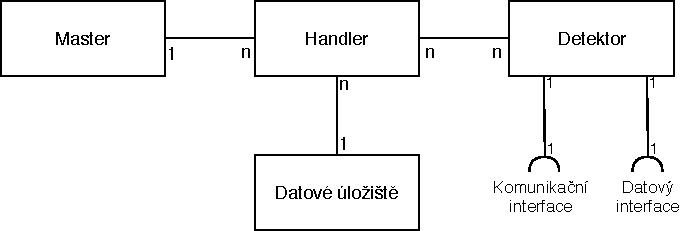
\includegraphics[width=14.5cm]{figures/arch_sw.pdf}
		\caption{Pixnet: softwarová architektura.}
		\label{fig:arch:sw_architecture}
	\end{center}
\end{figure}

V následujících podkapitolách budou detailněji popsány jednotlivé komponenty z obrázku~\ref{chap:arch:sw}.
\subsection{Detektor}\label{chap:arch:sw:detector}
Detektor je logická jednotka systému, která je reprezentována implementací komunikačního a datového interface, konfigurací a svým stavem. Fyzické propojení s detektorem je realizováno implementací komunikačního interface.

Komunikační interface obsahuje například metody pro navazování spojení s detektorem, metody pro nahrávání konfigurace a metody pro získání podporovaných příkazů detektoru a jejich vykonání. Každý příkaz má svoje ID, název a model vstupních a výstupních hodnot. Modelem hodnot rozumíme množinu parametrů různých datových typů (\texttt{boolean}, \texttt{integer}, \texttt{float} apod.), které mohou nabývat hodnot omezených zadaným intervalem, nebo jedné z předdefinovaných diskrétních hodnot.

Datový interface obsahuje kromě inicializačních metod (předání konfigurace detektoru apod.) také metodu pro předání reference na asynchronní frontu naměřených dat, do které jsou data vkládána implementací komunikačního interface. Datový interface může mít několik implementací -- například data mohou být ukládána do datového úložiště handleru a následně asynchronně nahrána do centrálního datového úložiště, nebo mohou být rovnou synchronně nahrávána do datového úložiště.

\subsection{Datové úložiště}
Klíčový požadavek na datové úložiště je škálovatelnost, jelikož pro sítě o vetším počtu detektorů by ukládání dat do jednoho uzlu znamenalo omezení maximálního datového toku, dané kapacitou daného uzlu.

Jednou z možností implementace může být využití distribuovaného souborového systému, například \textit{Hadoop Distributed File System} \cite{HDFS}, který se v praxi\footnote{například v roce 2010 internetová společnost \textit{Yahoo!} používala \texttt{HDFS} pro persistenci \unit{25}{PB} podnikových dat \cite{HDFS}.} používá pro distribuované ukládání dat s možností jejich redundance na více uzlech (pro potřeby zálohování). 

Další možností může být použití některé z \texttt{NoSQL} distribuovaných databází, například \textit{MongoDB} (viz \ref{chap:arch:technologie:mongodb}).

\subsection{Handler}
Handler je komponenta, kterou je řízena podmnožina detektorů detektorové sítě. K jednomu handleru je tedy možné připojit $n$ detektorů, kde $n$ je omezeno sumou datového toku přes všechny připojené detektory v závislosti na maximálním možném datovém toku handleru.

Handler komunikuje s detektorem pomocí dodané implementace jeho komunikačního interface a data detektorem vygenerovaná jsou pomocí implementace datového interface uložena do datového úložiště, nebo zpracována jiným způsobem.

Handler je zodpovědný za zavedení dodaných implementací komunikačního a datového interface do systému. Například po přiřazení detektoru handleru, handler získá seznam podporovaných příkazů detektoru a poskytne je masteru. To systému umožňuje řízení heterogenní sítě detektorů homogenním způsobem, jak již bylo zmíněno v \ref{chap:arch:motivation}.

Aby bylo možné handlery, potažmo detektory, řídit centralizovaně, handler poskytuje \texttt{API}\footnote{Z angl. \textit{Application programming interface} (aplikační programové rozhraní).}. Pomocí \texttt{API} jsou jednotlivé handlery připojovány do systému, handlerům jsou přiřazovány a odebírány detektory, inicializuje se konfigurace detektorů a je řízena akvizice dat.

\subsection{Master}
Master je centrální prvek systému, jehož prostřednictvím jsou řízeny handlery. Master poskytuje \texttt{API} pro své řízení pomocí pomocí frontendové aplikace. Tato aplikace je webový tenký klient, který uživateli poskytuje uživatelské rozhraní pro řízení systému.

Když uživatel přidává nový detektor do systému, tak nejprve skrze uživatelské rozhraní frontend aplikace zadá parametry detektoru, včetně implementace komunikačního a datového rozhraní, jak je znázorněno na obr. \ref{fig:arch:handler:new_detector}. Poté je detektor nahrán do mastera pomocí jeho \texttt{API}, kde je následně perzistentně uložen do jeho databáze. Při přiřazování detektoru handleru je konfigurace detektoru včetně implementace komunikačního a datového interface nahrána do zvoleného handleru, kde je dále zpracována. Zpracování konfigurace probíhá v následujících krocích:
\begin{enumerate}
    \item Vytvoření instance komunikačního interface a ověření jeho validity.
    \item Vytvoření instance datového interface a ověření jeho validity.
    \item Syntaktická analýza (tzv. \textit{parsing}) konfigurace detektoru a její nahrání do instancí komunikačního a datového interface.
    \item Vytvoření asynchronní fronty měřených dat a její předání instancím komunikačního a datového interface.
\end{enumerate}
Po dokončení inicializační sekvence je uživatel notifikován a v případě úspěšného dokončení je detektor připraven vykonávat příchozí příkazy a měřit data.

\begin{figure}[th!]
	\begin{center}
		\begin{sequencediagram}
            \newthread[blue_ligh]{mf}{Master frontend}
            \newinst[0.5]{mb}{Master backend}
            \newinst[0.5]{h}{Handler}
            \newinst[0.5]{d}{Detektor}
            \newinst[0.19]{c}{\shortstack{Impl kom.\\interface}}
            \newinst[0.19]{p}{\shortstack{Impl dat.\\interface}}
            
            % nahrání konfigurace
            \postlevel
            \begin{call}{mf}{
                %pro úpravu thread color
                %\tikzset{threadstyle/.style={top color=white,bottom color=red}}
                    \shortstack{
                        Přidání nového\\
                        detektoru
                    }
                }{mb}{výsledek}
                
                \begin{callself}{mb}{\shortstack{Validace a uložení\\konfigurace detektoru}}{výsledek}
                    \postlevel
                \end{callself}	
                
            \end{call}

            % binding
            \postlevel
            \postlevel
            \begin{call}{mf}{\shortstack{Přiřazení detektoru\\handleru}}{mb}{výsledek}
                
                \postlevel
                \begin{call}{mb}{\shortstack{Přiřazení\\detektoru}}{h}{výsledek}
                    
                    \begin{call}{h}{\shortstack{Inicializace}}{d}{výsledek}
                        
                        \begin{call}{d}{\shortstack{Inicializace\\(konfig.,\\fronta dat)}}{c}{}
                        \end{call}
                        
                        \postlevel
                        \postlevel
                        \begin{call}{d}{\shortstack{Inicializace\\(konfig., fronta dat)}}{p}{}
                        \end{call}

                        %\begin{call}{d}{\shortstack{Zavedení\\modulu}}{c}{}
                        %\end{call}
    
                        %\begin{call}{d}{\shortstack{Zavedení modulu}}{p}{}
                        %\end{call}

                        %\postlevel
                        %\begin{call}{d}{\shortstack{Nahrání\\konfigurace}}{c}{}
                        %\end{call}

                        %\begin{call}{d}{\shortstack{Nahrání konfigurace}}{p}{}
                        %\end{call}
        
                        %\begin{messcall}{d}{\shortstack{Fronta dat}}{c}
                        %\end{messcall}

                        %\begin{messcall}{d}{\shortstack{Fronta dat}}{p}
                        %\end{messcall}
        
                    \end{call}
        
                \end{call}

            \end{call}
            
		\end{sequencediagram}
		\caption{Sekvenční diagram znázorňující příklad přidání detektoru do systému a jeho přiřazení handleru.}
		\label{fig:arch:handler:new_detector}
	\end{center}
\end{figure}

Jako datové úložiště pro konfigurace detektorů, informace o jejich stavu a o stavu jednotlivých handlerů bude navržena relační \texttt{SQL}\footnote{Z angl. \textit{Structured Query Language} (strukturovaný dotazovací jazyk).} databáze, ke které bude přistupovat pouze backend mastera.

%********************************************************************************
% Hardwarová architektura
%********************************************************************************
\section{Hardwarová architektura}\label{chap:arch:hw}
V předchozí podkapitole byla popsána softwarová architektura. Fyzická instalace sítě přináší další omezení, především z pohledu síťové infrastruktury, která budou popsána v této podkapitole.

Na obrázku \ref{fig:arch:hw_architecture} je příklad sítě sestávající se ze dvou podsítí (tzv. \textit{subnetwork}). Podsítí rozumíme takovou podmnožinu detektorů a handlerů, ve které libovolný detektor může být přiřazen libovolnému handleru. Pro úplnost je třeba doplnit, že nutnou podmínkou je, aby všechny handlery měly spojení s masterem a s distribuovaným úložištěm naměřených dat.

\begin{figure}[h]
	\begin{center}
		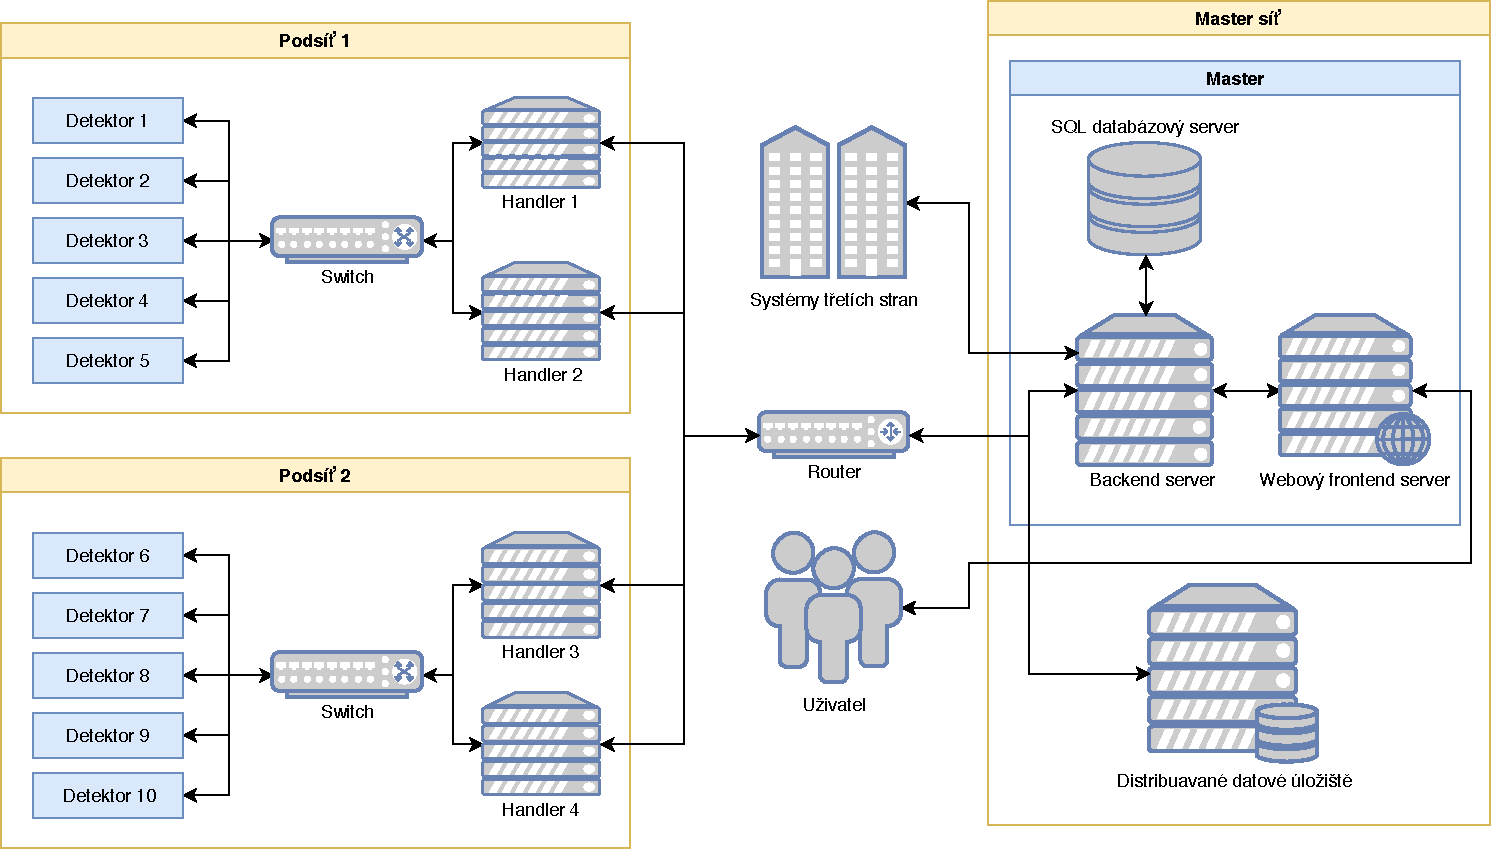
\includegraphics[width=15cm]{figures/arch_hw.pdf}
		\caption{Pixnet: hardwarová architektura s příkladem realizace sítě o dvou podsítích, kde v každé jsou dva handlery a pět detektorů, mastera (s \textit{SQL} databází pro persistenci konfigurace a frontend server poskytující webovou aplikaci) a centrálního datového úložiště naměřených dat.}
		\label{fig:arch:hw_architecture}
	\end{center}
\end{figure}

Master se skládá ze tří komponent:
\begin{description}
    \item[Backend server] implementující business logiku pro komunikaci s handlery (jako například přiřazování detektorů, řízení akvizice dat apod.). Server zároveň poskytuje \textit{API} pro možnou integraci s webovým frontend serverem se systémy třetích stran\footnote{Například pro experiment \textit{ATLAS-TPX} v CERN je plánována integrace s \texttt{DCS} \cite{cern_dcs} (\textit{Detector Control System}), který umožňuje centrální řízení detektorových systému, včetně integrace do bezpečnostního systému \texttt{DSS} (\textit{Detector Safety System}), datového akvizičního systému \texttt{DAQ} (\textit{Data Acquisition System}) apod.}, kterými muže být plnohodnotně řízen.
    \item[Databázový server] poskytující relační \texttt{SQL} databázi pro persistenci konfigurace systému, včetně implementace potřebných rozhraní, stavových informací sítě apod.
    \item[Frontend server] poskytující webovou aplikaci s uživatelským rozhraním pro řízení mastera pomocí jeho \texttt{API}, resp. pro řízení celé sítě.
\end{description}

Na příkladu zmíněném výše je síť využívající jedno centrální datové úložiště. Realizace této komponenty je závislá na poskytnuté implementaci datových rozhraní jednotlivých detektorů. Může být implementovaná pomocí centralizovaného, nebo distribuovaného systému. Umístění úložiště také není omezeno -- může být umístěno v síti mastera, v jednotlivých podsítích, v síti mastera i v jednotlivých podsítích (buffer pro malou šířku pásma spojení podsíť -- master síť), nebo třeba v internetu (cloudové úložiště, jako například \textit{Firebase Firestore}, \textit{Amazon 3S}, \textit{Microsoft Azure} apod.).

%********************************************************************************
% Škálovatelnost
%********************************************************************************
\section{Škálovatelnost}
Škálování systému Pixnet teoreticky není omezeno. Kritickým bodem každého datového akvizičního systému je vyčítání a ukládání naměřených dat. Tento problém je řešen horizontálním škálováním, spočívajícím v přidáváním handlerů, které zajišťují komunikaci s detektory a ukládání naměřených dat.

Možnost škálování datového úložiště je závislá na instanci hardwarové architektury popsané výše. V \cite{gandini2014performance} bylo ukázáno, že \texttt{NoSQL} databázové systémy (jako například \textit{MongoDB} nebo \textit{Apache Cassandra}) jsou dobře horizontálně škálovatelné a jsou schopny zajistit dostatečnou rychlost zápisu vstupních dat. Takže například pro instanci sítě s vhodně zvoleným distribuovaným datovým úložištěm, umístěným v síti mastera (viz obr. \ref{fig:arch:hw_architecture}), budou požadavky na persistenci naměřených dat splněny.

%********************************************************************************
% Použité technologie
%********************************************************************************
\section{Použité technologie}\label{chap:arch:technologie}
V této podkapitole jsou stručně shrnuty technologie použité při implementaci systému.

\begin{description}
    \item[Java] je staticky typovaný, objektově orientovaný programovací jazyk a byl při zahájení implementace zvolen jako primární programovací jazyk pro vývoj tohoto systému. Byl zvolen především pro svou jednoduchost, výkonost a přenositelnost. 
    
    Java je interpretovaný programovací jazyk -- při kompilaci kód není kompilovaný do strojového kódu zvolené platformy, ale do tzv. \textit{bytecode}, který je platformně nezávislý. \textit{Bytecode} pak může být spuštěn na libovolném počítači či zařízení, které disponuje interpretem Javy -- \texttt{JVM} (\textit{Java Virtual Machine}). Java není čistě interpretovaný programovací jazyk, protože v pozdějších verzích byla přidána podpora pro \texttt{JIT} (tzv. \textit{Just-in-time}) kompilátoru, který umožňuje dynamickou kompilaci \textit{bytecode} do strojového kódu dané platformy, díky čemuž může Java ve srovnání s neinterpretovanými programovacími jazyky (\texttt{C++} apod.) dosahovat srovnatelných výsledků.
    
    Java také obsahuje nástroj pro generační správu paměti (tzv. \textit{Garbage Collector}), který se stará o automatické uvolňování paměti mazáním objektů, na které neukazuje žádná reference. Tento nástroj je pro dlouhodobě běžící serverové systémy velice užitečný.

    \item[Kotlin]\label{chap:arch:technologie:kotlin} je moderní staticky typovaný, objektově orientovaný programovací jazyk, který běží nad \texttt{JVM}. Hlavní výhoda Kotlinu je jeho interoperabilita -- kód může být zkompilovaný do Java \textit{bytecode}, do JavaScriptu, nebo i do nativního kódu s tím, že může používat závislosti dané platformy (například pro kompilaci do Java \textit{bytecode} může používat Java knihovny, takže část kompilovaného kódu může být napsána v Javě a část v Kotlinu).

    Oproti Javě poskytuje mnoho výhod, jako například \textit{null-safety} (každá proměnná má kromě svého datového typu i příznak, jestli může být \texttt{null}, což eliminuje spoustu chyb, se kterými se můžeme setkat například v Javě), podpora funkcionálního stylu programování (oproti Javě může být v proměnné uložená funkce), \textit{extension functions} (podobně jako v \texttt{C\#}, je možné přidat funkci do dané třídy bez nutnosti její modifikace, nebo vytvořené poděděné třídy) a další vylepšení. 
    
    Především díky výhodám popsaným výše bylo v pozdější fázi vývoje rozhodnuto o použití Kotlinu, coby primárního programovacího jazyku pro handler a backend mastera. Také bylo experimentováno s použitím Kotlinu pro frontend mastera, pomocí vytvoření společné \textit{code-base} pro backend a frontend mastera (sestávajícího se z business logiky a modelu), ale od tohoto přístupu bylo upuštěno z důvodů omezené podpory kompilátoru Kotlin kódu do JavaScriptu a z důvodu omezené komunitní podpory.
    
    \item[JavaScript] je interpretovaný, objektově orientovaný programovací jazyk, který je zpravidla používán pro tvorbu webových aplikací, ale má i jiná využití. V kontextu webových aplikací, JavaScript kód je interpretován na klientské straně v prohlížeči a pomocí jeho \textit{API} manipuluje s načtenou HTML stránkou, resp. její vnitřní interpretací webovým prohlížečem -- tzv. \texttt{DOM} (\textit{Document Object Model}).
    
    V rámci této práce je použit pro implementaci frontendové části mastera -- webové aplikace poskytující uživatelské rozhraní pro obsluhu systému Pixnet.
     
    \item[Gradle] Je automatizovaný build\footnote{Sestavování počítačových programů.} systém, který vychází z \textit{Apache Ant} a \textit{Apache Maven} a používá \texttt{DSL}\footnote{Z angl. \textit{domain-specific language} (doménově specifický jazyk)} (založeném na \textit{Groovy} a \textit{Kotlin}). Umožňuje automatizované stahování a správu závislostí a knihoven z online repositářů (kromě \textit{Gradle} i \textit{Maven} a \textit{Ivy} pro kompatibilitu s dalšími build systémy).
    
    \item[Spring]\label{chap:arch:technologie:spring} je aplikační framework pro vývoj \texttt{J2EE}\footnote{Označení pro Java \textit{Enterprise Edition} -- platformy pro vývoj podnikových systémů, odvozené od JavaSE (Standard Edition)} aplikací a v rámci systému Pixnet bude použit v rámci implementace handlera a mastera. Spring framework je sada modulů, které nabízejí nástroje jako například webový controller (pro poskytování \texttt{REST API}), \textit{Dependency Injection}\footnote{Technika pro vkládání závislostí mezi komponentami počítačového programu, aniž by v době kompilace měly komponenty na sebe referenci.}, JPA (\textit{Java Persistent API} pro práci s databází), podporu testování apod.

    Novější alternativou je Spring Boot, který je nadstavbou nad původním Spring frameworkem. Spring Boot odstraňuje nutnost komplikovaného definování konfigurace a také přináší možnost zapouzdření do samostatně spustitelné aplikace s embedovaným webovým serverem (\textit{Tomcat}, nebo \textit{Jetty}), takže již není třeba nasazovat \texttt{WAR}\footnote{Z angl. \textit{Web Application Archive} (archív se zkompilovanou webovou \texttt{J2EE} aplikací).} na webový server, protože Spring Boot aplikace je zkompilovatelná do spustitelné \texttt{JAR}\footnote{Z angl. \textit{Java Archive} (archív se zkompilovanou Java aplikací).} aplikace.
    
    \item[ReactJS]\label{chap:arch:technologie:react} je JavaScriptová knihovna pro vývoj uživatelského rozhraní webových aplikací, vyvíjená společností Facebook. React je používán k vývoji tzv. \textit{single-page} aplikací, tj. takových webových aplikací, které k interakci s uživatelem používají jen jednu stránku, jejíž obsah dynamicky přepisují (na rozdíl od stahování nové stránky z webového serveru).
    
    React je založen na principu zapouzdřených komponent, kde každá komponenta má svoje vlastnosti a svůj stav. Komponenty jsou znovupoužitelné a zanořitelné do jiných komponent. Navíc komponenty nepracují přímo s DOM prohlížeče, ale přistupují pouze k jeho virtuální reprezentaci, což umožňuje optimalizovat operace s DOM. Například když nějaká komponenta změní svůj stav (ev. tranzitivně i stav jiných komponent), tak se na stránce přegenerují jen takové komponenty, jejichž stav byl změněn.

    React bude použit pro implementaci frontendové webové aplikace mastera. Vedle Reactu existuje ještě React Native, který je určen pro hybridní vývoj mobilních aplikací, tím se ale v této práci nebudeme zabývat.
    
    \item[PostgreSQL]\label{chap:arch:technologie:postgresql} je nejpoužívanější open source objektově-relační databázový systém. Oproti klasickým relačním databázím (například \textit{MySQL}) má objektově orientovaný databázový model, který je přímo podporován databázovým schématem a dotazovacím jazykem.
    
    Tento databázový systém bude použit pro persistenci konfigurace sítě a bude k němu přistupovat backend mastera.
    
    \item[MongoDB]\label{chap:arch:technologie:mongodb} je \texttt{NoSQL} dokumentový databázový systém. Oproti tradičním relačním databázovým systémům jsou data ukládána do \texttt{BSON}\footnote{Binární forma JSON (z ang. JavaScript Object Notation)} dokumentů. Mezi hlavní výhody \textit{MongoDB} patří:

    \begin{description}
        \item[Indexace:] Na každé pole objektů v dokumentu lze vytvořit index a tím zrychlit vyhledávání v datech.
        \item[Replikace:] \textit{MongoDB} ukládá data do tzv. \textit{replica set}, která obsahuje jednu, nebo více replik dat. Pro případ více replik, jedna vždy funguje jako primární a ostatní jako sekundární, do kterých jsou replikována data z primární repliky. Hlavní výhoda spočívá ve vyšší dostupnosti dat (data lze číst z více replik současně) a spolehlivosti (když jedna replika selže, je nahrazena replikou jinou).
        \item[Horizontální škálování:] \textit{MongoDB} má podporu pro horizontální škálování pomocí tzv. \textit{shardingu} \cite{mongodb-scale}. \textit{Sharded cluster} je pak množina uzlů s jednotlivými \textit{shardy}, kde každý obsahuje podmnožinu \textit{shardovaných} dat.
    \end{description}

\end{description}
\addbibresource{reference.bib}

\chapter{Handler}\label{chap:handler}

V této kapitole bude čtenář podrobně seznámen s handlerem - komponentou pro distribuované řízení detektorů. Jak již bylo zmíněno v kapitole \ref{chap:arch}, handler je komponenta zajišťující komunikaci a vyčítání dat z detektorů (viz obr. \ref{fig:handler:overview}) skrze poskytnuté implementace komunikačního a datového interface.
  
Handler implementuje \textit{Spring framework} (viz \ref{chap:arch:technologie:spring}), aby mohl poskytovat \texttt{REST API} pro management detektorů a pro poskytování stavových informací o své instanci. Handler dále poskytuje jednoduché webové rozhraní s přehledem připojených detektorů.

Na obrázku \ref{fig:handler:overview} je znázorněn příklad instance handleru z pohledu vstupu (pět přiřazených detektorů) a pohledu výstupu (poskytované \texttt{REST API} a webové rozhraní.)

\begin{figure}[bh]
	\begin{center}
		\vspace*{1cm}
		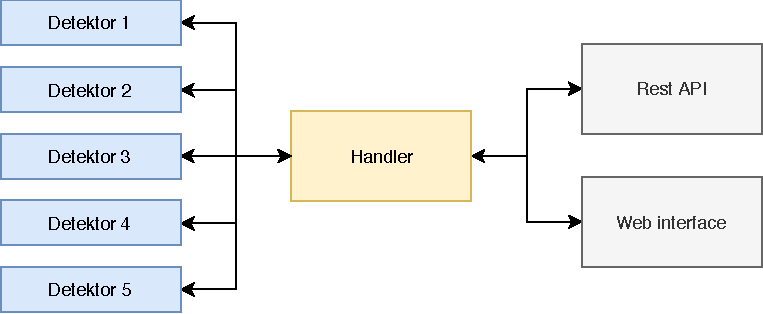
\includegraphics[width=14cm]{figures/handler_overview.pdf}
		\caption{Pixnet - handler: příklad instance handleru s pěti připojenými detektory, poskytujícího REST API pro své řízení a webové uživatelské rozhraní s přehledem připojených detektorů.}
		\label{fig:handler:overview}
	\end{center}
\end{figure}

\newpage

%********************************************************************************
% Vrstvy softwarové architektury
%********************************************************************************
\section{Vrstvy softwarové architektury}\label{chap:handler:architecture}
Tato podkapitola je věnována softwarové architektuře handleru. Budou zde představeny jednotlivé její vrstvy, tj. od vrstvy pro komunikaci s detektorem, management detektorů, Spring implementaci, až po výstupní vrstvu poskytující \texttt{REST API} a webové rozhraní - viz obr. \ref{fig:handler:arch}. Vybrané vrstvy budou popsány detailněji v dalších podkapitolách.

\begin{figure}[th]
	\begin{center}
		\vspace*{0.4cm}
		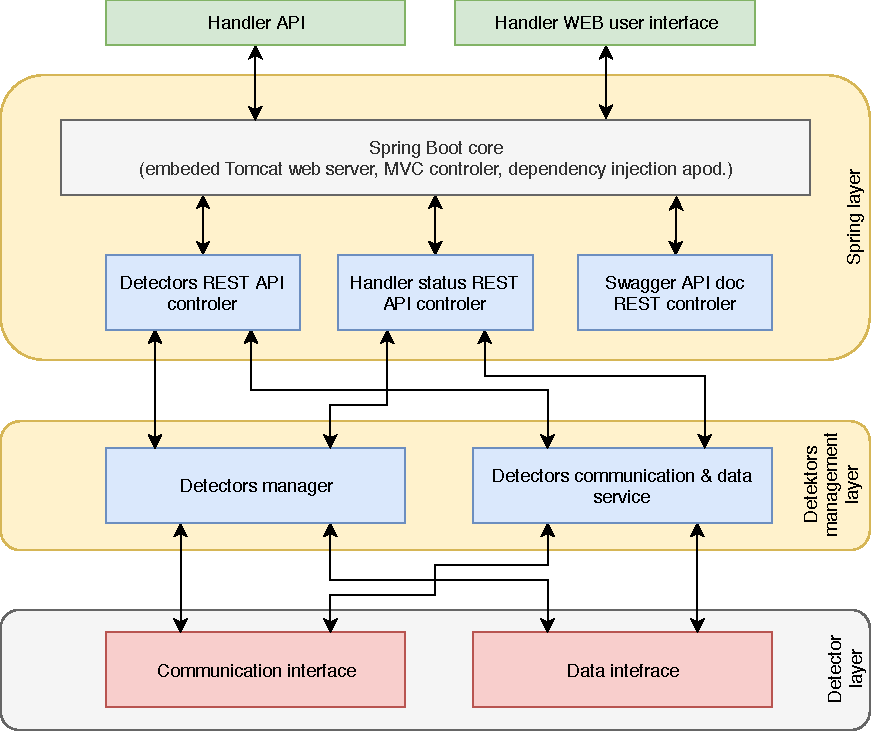
\includegraphics[width=14cm]{figures/handler_architecture.pdf}
		\caption{Pixnet - handler: softwarová architektura s vrstvami pro (i) rozhraní detektoru (\textit{Detector layer}), (ii) management detektorů (\textit{Detectors management layer}),(iii) Spring vrstvu (\textit{Spring layer}) a (iv) výstupní vrstvou pro \texttt{REST API} a webové uživatelské rozhraní.}
		\label{fig:handler:arch}
	\end{center}
\end{figure}

%********************************************************************************
% Vrstvy softwarové architektury - Detektorová vrstva
%********************************************************************************
\subsection{Detektorová vrstva}\label{chap:handler:detector_layer}
Detektorová vrstva se skládá ze dvou částí - externě poskytnuté implementace komunikačního a datového interface. Tyto tzv. moduly jsou zavedené až za běhu programu pomocí vyšších vrstev systému.

\subsubsection{Zavádění modulů}\label{chap:handler:detector_layer:module_init}
Každý modul, obsahující implementaci komunikačního, nebo datového interface, musí pro své zavedení do systému splňovat následující kritéria:

\begin{itemize}
	\item Musí být zkompilován do Java archívu (\texttt{*.jar}) - současná verze implementace podporuje pouze moduly vyvinuté v jazyce Java (resp. také v jazyce Kotlin, zkompilovaného do Java \textit{bytecode}), v dalších verzích je plánováno přidání podpory pro \texttt{C++} a \texttt{Python}.
	\item Při vývoji modulu musí být použit datový model, který je součástí poskytovaných knihoven.
	\item Modul musí obsahovat implementaci jednoho z již zmíněních rozhraní. Navíc, celý název implementující třídy (vč. tzv. \texttt{package}) musí být uveden jako atribut s názvem \texttt{PluginImplClass} v manifestu \texttt{jar} archívu, viz zdrojový kód \ref{src:handler:manifest}.
\end{itemize}

\begin{code}[h!]
\begin{minted}[
  frame=single,
	linenos,
	breaklines
  ]{html}
  Manifest-Version: 1.0
  PluginImplClass: cz.ctu.ieap.pixnet.handler.detector_communication_katherine.CommImpl  
\end{minted}
\caption{Příklad obsahu souboru \texttt{MANIFEST.MF}, obsaženého v \texttt{jar} archívu modulu.}
\label{src:handler:manifest}
\end{code}

%********************************************************************************
% Vrstvy softwarové architektury - Detektorová vrstva - Komunikační rozhraní
%********************************************************************************
\subsubsection{Komunikační rozhraní}\label{chap:handler:detector_layer:commIntf}
Zdrojový kód \ref{src:handler:comm_intf} obsahuje interface, který komunikační modul detektoru musí implementovat.

Prvních pět metod (tj. řádek 3 až 7) má čistě informativní charakter a jejich implementace má čistě informativní charakter pro operátora systému.

Na řádcích 8 a 9 je setter a getter pro konfiguraci detektoru. Konfigurace je detektoru předána jako \texttt{String}\footnote{Datový typ obsahující textový řetězec} (setter) a musí být do něj serializovatelná (getter). Systém ale s konfigurací detektoru neumí pracovat (kromě komunikačního modulu detektoru, resp. implementace komunikačního interface), tudíž jejíž syntax není vynucována a její podoba je čistě v kompetenci poskytovatele komunikačního modulu. Avšak je doporučeno, aby zvolený formát byl strojově i lidsky čitelný, z důvodu jeho snazší editace\footnote{V dalších fázích implementace systému je plánováno přidání podpory editace konfigurace v rámci webového uživatelského rozhraní mastera.}. Takový formát může být například \texttt{JSON}\footnote{Z angl. \textit{JavaScript Object Notation} (JavaScriptový objektový zápis).}, nebo \texttt{YAML}\footnoteUrl{http://yaml.org/}, který je použit pro serializace konfigurace komunikačního modulu Katherine (viz \ref{chap:katherine:comm}).

\begin{code}[h!]
\begin{minted}[
    frame=single,
	linenos,
	breaklines
  ]{kotlin}
interface DetectorComm {

  fun getDetectorType(): DetectorType
  fun getReadoutName(): String
  fun getSensorsCount(): Int
  fun getDetectorWidth(): Int
  fun getDetectorHeight(): Int
  fun setDetectorConfig(config: String)
  fun getDetectorConfig(): String?
  fun getSupportedValueCommands(): List<AbstractValueCommand>
  fun getSupportedExecutionCommands(): List<AbstractExecutionCommand>
  fun getAcceptedFilesKeys(): List<String>
  fun getDataFrameQueue(): BlockingQueue<AbstractDataFrame>
  
  fun isConnected(): Boolean
  fun connect(): Boolean
  fun disconnect(): Boolean
  
  fun executeSetValueCommand(commandID: Int, payload: ValuePayload)
  fun executeGetValueCommand(commandID: Int): ValuePayload
  fun executeExecutionCommand(commandID: Int, input: Map<String, ValuePayload>): Map<String,  ValuePayload>
  fun uploadFile(fileKey: String, file: ByteArray)
  fun setCallback(callback: Callback)
  
  interface Callback {
    val classLoader: ClassLoader?
  }

}
\end{minted}
\caption{Komunikační interface detektoru, napsané v jazyce Kotlin (viz \ref{chap:arch:technologie:kotlin})).}
\label{src:handler:comm_intf}
\end{code}

Pro získání seznamu podporovaných \textit{value commands} (tj. příkazů pro operace s jednotlivými hodnotami detektoru) slouží metoda \texttt{getSupportedValueCommands()}, viz řádek 10. \texttt{AbstractValueCommand} má v modelu poskytované knihovny dvě implementace:
\begin{enumerate}[label=(\roman*)]
	\item \texttt{ValueCommand} obsahuje atributy pro daného příkazu, tj.:
	\begin{itemize}
		\item \textbf{id} - celočíselný unikátní identifikátor daného příkazu,
		\item \textbf{name} - název příkazu, resp. manipulované hodnoty detektoru,
		\item \textbf{valueUnit} - jednotka veličiny manipulované hodnoty detektoru (může nabývat hodnot z \textit{Enum} třídy \texttt{ValueUnit} poskytovaného modelu, např. \texttt{ValueUnit.VOLT} apod.),
		\item \textbf{accessType} - modifikátor přístupu manipulované hodnoty, který může nabývat těchto hodnot:
		\begin{description}
			\item[\texttt{SETTER}] pro takové hodnoty, které je možné pouze nastavovat,
			\item[\texttt{GETTER}] pro takové hodnoty, které je možné pouze číst a
			\item[\texttt{SETTER\_AND\_GETTER}] pro hodnoty, které je možné nastavovat i číst.
		\end{description}
		\item \textbf{valueModel} - datový model hodnoty daného příkazu, který definuje datový typ veličiny (podporovány jsou \texttt{Boolean}, \texttt{String}, \texttt{Integer}, \texttt{Long}, \texttt{Float} a \texttt{Double}) a omezení rozsahu hodnot. Model může být diskrétní (tzn. hodnota může nabývat jen nějaké z předem definovaných hodnot), nebo spojitý (hodnota může nabývat jakékoliv hodnoty ze zadaného intervalu).
	\end{itemize}
	Viz zdrojový kód \ref{src:handler:value_command} pro příklad definice \textit{ValueCommand} pro \textit{bias} (prahové napětí detektoru).

	\item \texttt{ValueCommandGroup} je třída pro seskupování příkazů podobného významu (např. \texttt{DAC} hodnoty detektoru) a obsahuje název skupiny příkazů a seznam jednotlivých\\\texttt{ValueCommands}.
\end{enumerate}

\begin{code}[h!]
\begin{minted}[
    frame=single,
	linenos,
	breaklines
  ]{java}
valueCommands.add(ValueCommand(
    42, // id
    "Bias", // name
    ValueUnit.VOLT, // valueUnit
    SETTER_AND_GETTER, // accessType
    FloatValueModel(-300f, 300f) // valueModel
))
\end{minted}
\caption{Příklad definice \textit{ValueCommand} detektoru pro příkaz s názvem \textit{"Bias"}, id 42, jednotkou Volt, modifikátorem přístupu \textit{Setter \& Getter} a reálným modelem hodnot, omezeným intervalem $<-300,300>$.}
\label{src:handler:value_command}
\end{code}

Pro vykonání \texttt{ValueCommand} je třeba implementovat metody \texttt{executeSetValueCommand()} a \texttt{executeGetValueCommand()}, viz řádky 19 a 20 komunikačního interface (zdrojový kód \ref{src:handler:comm_intf}). První metoda slouží pro nastavení hodnot a akceptuje ID příkazu a \texttt{valuePayload}, který obsahuje hodnotu jednoho ze šesti podporovaných datových typů, a je možné jej vykonat pouze pro příkazy, které mají \texttt{accessType}, umožňující zápis hodnot. Druhá metoda slouží pro čtení hodnot, jako vstupní parametr má ID příkazu a její návratový typ je \texttt{ValuePayload}, obsahující hodnotu čteného parametru.

Dalším typem příkazů je získání seznamu podporovaných \texttt{ExecutionCommands} (viz 11. řádek komunikačního interface \ref{src:handler:comm_intf}). Od \texttt{ValueCommands} se liší tím, že vstup a výstup není omezen stejnou veličinou (resp. jejím modelem hodnot) a ani jejich množstvím. Tento přístup tedy umožňuje definovat příkazy, které mají 0 až m vstupních hodnot a 0 až n výstupních hodnot. Obdobně jako \texttt{AbstractValueCommand}, i \texttt{AbstractExecutionCommands} má v poskytované knihovně dvě implementace:
\begin{enumerate}[label=(\roman*)]
	\item \texttt{ExecutionCommand} je definován obdobně jako \texttt{ValueCommand} - má své ID, jméno, ale také obsahuje seznamy rozšířených modelů hodnot - jeden vstupní a jeden výstupní. Rozšířený model hodnot obsahuje již zmíněný \texttt{valueModel}, dále pak jméno hodnoty, její ID (textový řetězec) a \texttt{valueUnit}.
	
	Zdrojový kód \ref{src:handler:execution_command} obsahuje příklad s \texttt{ExecutionCommand} pro nastavení akvizičního módu detektoru. Z příkladu je patrné, že příkaz akceptuje právě dvě vstupní hodnoty (akviziční mód a \textit{FastVCO} přepínač) a že žádné hodnoty nevrací.
	
	\item \texttt{ExecutionCommandGroup} je obdobou třídy \texttt{ValueCommandGroup} pro \texttt{ExecutionCommand}. Obsahuje název skupiny příkazů a jejich seznam.
\end{enumerate}

\begin{code}[h!]
\begin{minted}[
    frame=single,
	linenos,
	breaklines
  ]{java}
executionCommands.add(ExecutionCommand(
  KatherineExecutionCommands.SET_ACQ_MODE.internalID, // ID (Int)
  "Set acquisition mode", // name
  // model vstupných hodnot
  arrayOf(
    ValueModelVerbose(
      "Acquisition mode", // název hodnoty
      ValueId.acq_mode.name, // ID hodnoty (String)
	  // celočíselný diskrétní model hodnot
	  IntValueModel(mapOf(
        Pair("ToA & ToT", 0),
        Pair("ToA", 1),
        Pair("Event & iToT", 2)
      )),
      ValueUnit.DIMENSIONLESS // jednotka hodnoty
    ), 
    ValueModelVerbose(
      "Fast vco enabled",
      ValueId.fast_vco_en.name,
      BooleanValueModel(mapOf(
        Pair("Enable", true),
        Pair("Disable", false)
      )),
      ValueUnit.DIMENSIONLESS
	)
  ),
  null // model výstupních hodnot
))
\end{minted}
\caption{Příklad definice \textit{ExecutionCommand} pro nastavování akvizičního módu detektoru s vyčítacím rozhraním \textit{Katherine} (viz \ref{chap:detectors:readouts:katherine}). Z příkladu je patrné, že vstupní model je tvořen dvěma hodnotami a výstupní model je prázdný.}
\label{src:handler:execution_command}
\end{code}

Pro vykonání \texttt{ExecutionCommand} slouží metoda \texttt{executeExecutionCommand()}, viz řádek 21 komunikačního interface (zdrojový kód \ref{src:handler:comm_intf}). Metoda akceptuje ID příkazu a mapu (tzn. seznam párů klíč - hodnota) jednotlivých hodnot. Klíčem v mapě je ID parametru a hodnota je již výše zmíněný \texttt{ValuePayload}, obsahující hodnotu parametru. Výstupem volání metody je pak mapa výstupních parametrů příkazu.

Pro přípojení detektoru, odpojení detektoru a zjišťování stavu připojení slouží metody \texttt{connect()}, \texttt{disconnect()} a \texttt{isConnected()} (viz řádky 15 až 17 zdrojového kódu \ref{src:handler:comm_intf}). Aby bylo možné provést jakoukoliv operaci interagující s detektorem (tj. vykonávání příkazů a nahrávání souborů) je nutné, aby byl detektor připojen, resp. metoda \texttt{isConnected()} musí vracet \texttt{true}.

Do detektorů rodiny \textit{Medipix} je třeba před jejich použitím nahrát konfiguraci jednotlivých pixelů detektoru. Konfigurace je pole bytů, kde nastavení jednoho pixelu je serializováno do jednoho bytu. Z tohoto důvodu je třeba přidat podporu pro nahrávání velkých binárních objektů (tzv. \texttt{LOB}\footnote{Z angl. Large Object.}).
Pro nahrávání souborů do detektoru slouží příkaz \texttt{uploadFile()} (viz řádek 22 zdrojového kódu \ref{src:handler:comm_intf}), který akceptuje ID souboru a jeho binární reprezentaci. Pro poskytnutí seznamu podporovaných souborů, resp. jejich ID, je třeba implementovat metodu \texttt{getAcceptedFilesKeys()} (viz řádek 12 zdrojového kódu \ref{src:handler:comm_intf}).

V kapitole \ref{chap:arch:sw:detector} již byl popsán tok měřených dat v handleru, resp. od komunikačního k datovému modulu. Přenos dat je realizován asynchronní blokující frontou (viz obr. \ref{fig:handler:data_queue}), tj. frontou ke které může asynchronně přistupovat více vláken současně a zároveň čtení z fonty je implementováno jako blokující operace (tzn. že zablokuje čtecí vlákno, než bude ve frontě nějaký element v vyčtení). Jelikož komunikační modul je zodpovědný za vytvoření instance fronty, tak její implementace je zcela v kompetenci poskytovatele komunikačního modulu. Jedinou podmínkou je, aby fronta implementovala interface \texttt{BlockingQueue}\footnote{Z \textit{Java Collections Framework}.}. V další části textu (viz \ref{chap:katherine}) bude čtenář seznámen s implementací komunikačního modulu s implementací fronty pomocí \texttt{LinkedBlockingQueue}\footnote{Implementace \texttt{BlockingQueue} pomocí spojového seznamu. V této frontě jsou elementy řazení pomocí FIFO (first-in-first-out). Fronty založené na spojové struktuře umožňují (ve srovnání s frontami založenými na dynamickém poly) vyšší datový tok, zejména pro vícevláknové aplikace.}.
\begin{figure}[h]
	\begin{center}
		\vspace*{0.5cm}
		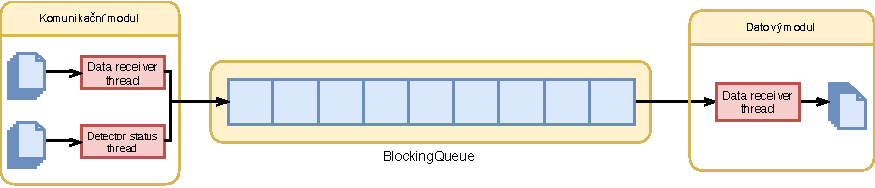
\includegraphics[width=14.5cm]{figures/handler_data_queue.pdf}
		\caption{Asynchronní blokující fronta naměřených dat s příkladem produkujících vláken v komunikačním modulu a přijímacím vláknu v datovém modulu.}
		\label{fig:handler:data_queue}
	\end{center}
\end{figure}

Poslední metodou komunikačního interface je metoda \texttt{setCallback()} (viz 23. řádek komunikačního interface (zdrojový kód \ref{src:handler:comm_intf})). Tato metoda je handlerem zavolána bezprostředně po inicializaci modulu a modul si může uložit referenci na předaný \texttt{callback} (instanci interface \texttt{Callback} z komunikačního interface). \texttt{Callback} slouží například k získání Java \texttt{ClassLoader}, kterým byl modul načten (používá se například pro parsing konfigurace).

%********************************************************************************
% Vrstvy softwarové architektury - Detektorová vrstva - Datové rozhraní
%********************************************************************************
\subsubsection{Datové rozhraní}\label{chap:handler:detector_layer:dataIntf}
Zdrojový kód \ref{src:handler:data_intf} obsahuje interface, které musí být implementováno datovým modulem detektoru.

\begin{code}[h!]
\begin{minted}[
  frame=single,
linenos,
breaklines
]{kotlin}
interface DataPersistence {

  fun setDataFrameQueue(queue: BlockingQueue<AbstractDataFrame>)
  fun setDetectorConfig(config: String)

  fun start()
  fun stop()

  fun setCallback(callback: Callback)

  interface Callback {
    val classLoader: ClassLoader?
  }

}
\end{minted}
\caption{Datový interface detektoru, napsané v jazyce Kotlin (viz \ref{chap:arch:technologie:kotlin})).}
\label{src:handler:data_intf}
\end{code}

Metoda \texttt{setDataFrameQueue()} (viz řádek 3) je zavolána po inicializaci modulu a jejím prostřednictvím handler předá datovému modulu frontu měřených dat, která byla vytvořena komunikačním modulem (viz předchozí komponenta).

Na 4. řádku je metoda pro předání konfigurace, které probíhá stejně, jako u komunikačního interface. Za tímto účelem je v datovém interface také \texttt{Callback} interface a metoda pro předání jeho instance, vytvořené handlerem. \texttt{Callback} obsahuje metodu pro předání \texttt{ClassLoader}, kterým byl modul zaveden.

Na řádcích 6 a 7 jsou metody \texttt{start()} a \texttt{stop()}, kterými se spouští a zastavuje vlákno zpracovávající frontu měřených dat.

%********************************************************************************
% Vrstvy softwarové architektury - Vrstva managementu detektorů
%********************************************************************************
\subsection{Vrstva managementu detektorů}\label{chap:handler:detectors_layer}
Vrstva pro management detektorů slouží jako úložiště detektorů a jako služba pro jejich řízení. Tato vrstva se skládá ze dvou komponent, které budou popsány v této podkapitole.

\begin{description}
  \item[\texttt{DetectorManager}] je komponenta, sloužící pro uložení detektorů přiřazených handleru do jeho paměti. Její instance je poskytována pomocí Java Bean Spring frameworkem jako \textit{singleton}, tzn. že v programu existuje pouze jedna instance této komponenty. Komponenta poskytuje úložiště detektorů, včetně \textit{CRUD}\footnote{Z angl. \textit{Create, read, update and delete} (vytváření, čtení, editaci a mazání).} operací nad jeho obsahem. Díky Spring frameworku, resp. jeho \texttt{Dependency-Injection} modulu lze tuto komponentu jednoduše použít z jiné komponenty systému.
  
  Detektor je reprezentován instancí třídy \texttt{Detector}, které má následující parametry:
  \begin{itemize}
    \item \texttt{}{detectorID} - unikátní textový identifikátor detektoru v systému,
    \item \texttt{name} - vlastní pojmenování detektoru (např. s označením fyzického umístění detektoru apod., nemusí být unikátní),
    \item \texttt{detectorComm} - instance komunikačního interface detektoru (viz \ref{chap:handler:detector_layer:commIntf}),
    \item \texttt{dataPersistence} - instance datového interface detektoru (viz \ref{chap:handler:detector_layer:dataIntf}),
    \item \texttt{pluginsClassLoader} - Java \texttt{ClassLoader}, kterým byly načteny výše zmíněné moduly a
    \item \texttt{status} - instance třídy \texttt{DetectorStatus}, ve které jsou uloženy stavové informace o detektoru (např. stav připojení, měření apod.).
  \end{itemize}
  
  \item[\texttt{DetectorService}] je komponenta poskytující operace nad detektorem, vč. navazování spojení, nahrávání souborů, vykonávání \textit{ValueCommands} a \textit{ExecutionCommands} apod. Komponenta je implementována jako \texttt{Service}\footnote{Dle \cite{Evans-domain-driven-design} \textit{Service} je množina operací, která není součástí modelu a zároveň není nositelem stavu.}.
\end{description}

%********************************************************************************
% Vrstvy softwarové architektury - Spring vrstva
%********************************************************************************
\subsection{Spring vrstva}\label{chap:handler:spring}
Tato vrstva se skládá z několika komponent, Spring Boot jádra a dalších knihoven Spring frameworku (viz obr. \ref{fig:handler:arch}). V této podkapitole bude čtenář seznámen s implementací jednotlivých komponent, tj. \textit{Detectors REST API controller} (viz \ref{chap:handler:spring:detectors_api}) pro správu a řízení detektorů masterem (ev. jinými systému), \textit{Handler status REST API controller} (viz \ref{chap:handler:spring:status_api}) pro zjišťování stavu handleru masterem, \textit{Swagger API doc REST controller} (viz \ref{chap:handler:spring:swagger}) pro webovou dokumentaci REST API poskytovaného handlerem a jednoduchého webového rozhraní handleru (viz \ref{chap:handler:spring:web}).

\subsubsection{Detectors REST API controller}\label{chap:handler:spring:detectors_api}
Tato komponenta je \texttt{RestController}, poskytující endpointy\footnote{Označení pro API metodu.} pro \textit{CRUD} operace nad detektory a jejich řízení. Komponenta je závislá na \texttt{DetectorManager} a \texttt{DetectorService} (viz \ref{chap:handler:detector_layer}). Všechny endpointy mají prefix URL cesty \texttt{/api/detector/}, takže například URL endpointu pro přidání detektoru může být \url{http://localhost:8082/api/detector/add}. Seznam API endpointů této komponenty je v tabulce \ref{tab:handler:api_detectors}.

\begin{table}[h]
	\begin{center}
		\begin{tabular}{|c|c|l|}
			\hline
      \textbf{HTTP} & & \\
      \textbf{Metoda} & \textbf{Endpoint} & \textbf{Popis} \\
			\hline
      GET & \texttt{/getAll} & Vrátí seznam všech detektorů \\
      GET & \texttt{/getById} & Vrátí detektor podle zadaného ID \\
      POST & \texttt{/add} & Přidá nový detektor \\
      DELETE & \texttt{/remove} & Odstraní detektor podle zadaného ID \\
      POST & \texttt{/connect} & Provede připojení zvoleného detektoru \\
      POST & \texttt{/disconnect} & Provede odpojení zvoleného detektoru \\
      POST & \texttt{/executeValueCommand} & Vykoná \texttt{ValueCommand} \\
      POST & \texttt{/executeExecutionCommand} & Vykoná \texttt{ExecutionCommand} \\
      POST & \texttt{/uploadFile} & Nahraje soubor do zvoleného detektoru \\
			\hline
		\end{tabular}
	\end{center}
	\caption{Endpointy komponenty \textit{Detectors REST API controller}.}
	\label{tab:handler:api_detectors}
\end{table}

Pro přenášená data je použil formát JSON. Zdrojový kód \ref{src:handler:detectors_api_example} znázorňuje ukázku API volání s příkladem s nastavením akvizičního módu detektoru (definice tohoto příkladu je uvedena ve zdrojovém kódu \ref{src:handler:execution_command}) pomocí \texttt{executeExecutionCommand} endpointu.

\begin{code}[h!]
\begin{minted}[
frame=single,
linenos,
breaklines
]{JavaScript}
> POST /api/detector/executeExecutionCommand HTTP/1.1
> Host: localhost:8082
> Content-Type: application/json
> Content-Length: 133
{
  "detectorID": "katherine_emulator",
  "commandID": 200,
  "input": {
    "acq_mode": {"intValue": 0},
    "fast_vco_en": {"booleanValue": false}
  }
}

< HTTP/1.1 200 
< Content-Type: application/json;charset=UTF-8
{
  "success": true
}
\end{minted}
\caption{Příklad volání API komponenty pro správu detektorů. V příkladu na řádcích 1 až 12 je \textit{request} pro vykonání \texttt{ExecutionCommand} pro nastavení akvizičního módu detektoru a na řádcích 14 až 18 je \textit{response} serveru.}
\label{src:handler:detectors_api_example}
\end{code}

Dokumentace k jednotlivým endpointům je poskytování jinou komponentou systému, viz kapitola \ref{chap:handler:spring:swagger}.

\subsubsection{Handler status REST API controller}\label{chap:handler:spring:status_api}
Tato komponenta je určena pro poskytování stavu handlerům dalším částem systému (např. master), ev. systémům třetích stran. Komponenta poskytuje jediný endpoint - \texttt{/status} (HTTP metoda \texttt{GET})). Ve zdrojovém kódu \ref{src:handler:status_api_example} je příklad volání tohoto endpointu, resp. JSON těla odpovědi. Z příkladu je patrné, že handler je online, má verzi software \texttt{0.0.0.1} a spravuje dva detektory.

\begin{code}[h!]
  \begin{minted}[
  frame=single,
  linenos,
  breaklines
  ]{JavaScript}
{
  "data": {
    "version": "0.0.0.1",
    "status": "ONLINE",
    "detectors": [
      {
        "id": "emulator_katherine",
        "name": "katherine emulator",
        "status": {
          "connection": "ONLINE",
          "measurement": "UNKNOWN"
        }
      },
      {
        "id": "katherine",
        "name": "katherine",
        "status": {
          "connection": "UNKNOWN",
          "measurement": "UNKNOWN"
        }
      }
    ]
  },
  "success": true
}
\end{minted}
\caption{Příklad volání API komponenty pro poskytování stavu handleru, resp. těla odpovědi endpointu \texttt{/status}.}
\label{src:handler:status_api_example}
\end{code}


\subsubsection{Swagger API doc REST controller}\label{chap:handler:spring:swagger}
Ke každému API je třeba poskytovat dokumentaci pro umožnění jeho implementace. Navíc, každá změna API by se měla současně projevit i v dokumentaci. Manuální udržování API dokumentace je pracné a náchylné na možné odchylky dokumentace od aktuálního stavu API. Proto bylo rozhodnuto použít automatizovaný nástroj na generování dokumentace.

Za tímto účelem byla implementována knihovna \textit{Springfox} \cite{springfox} - nástroj pro generování strojově i lidsky čitelné dokumentace. \textit{Springfox} je založen na \textit{OpenAPI}\footnote{\textit{OpenAPI Specification} (dříve \textit{Swagger Specification}) je formát pro popis REST API.} specifikaci a \textit{Swagger}\footnote{Nadstavba nad \textit{OpenAPI} umožňující návrh, vytváření (resp. generování serverového i klientského kódu), dokumentaci a testování REST API.} frameworku. \textit{Springfox} po spuštění aplikace automaticky analyzuje její komponenty a jednotlivé její třídy pomocí Java reflexe. Na základě analýzy potom vytvoří sémantický model jednotlivých endpointů.

Výstupem je pak online webová dokumentace, dostupná pomocí \texttt{swagger-ui.html} endpointu (tzn. url dokumentace je například \url{http://localhost:8082/swagger-ui.html}, dle konfigurace - viz \ref{chap:handler:config}) - viz obrázek \ref{fig:handler:swagger}. Webové rozhraní poskytuje nejen přehled všech endpointů včetně jejich parametrů, ale i definici datového modelu a nástroj pro manuální volání jednotlivých endpointů.
Endpoint pro stažení JSON OpenAPI specifikace je \texttt{/v2/api-docs}.

\begin{figure}[h]
	\begin{center}
    \begin{subfigure}{7.0cm}
			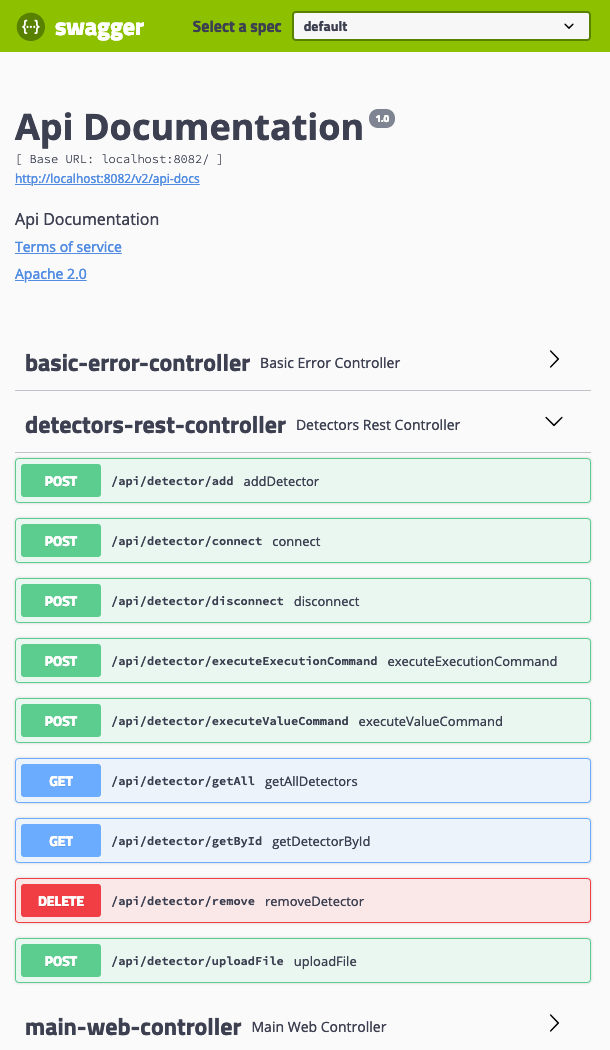
\includegraphics[width=7.0cm]{figures/handler_swagger_a.png}	
			\caption{Přehled endpointů.}
			\label{fig:handler:swagger_b}
		\end{subfigure}
		\hspace{0.1cm}
		\begin{subfigure}{7.0cm}
			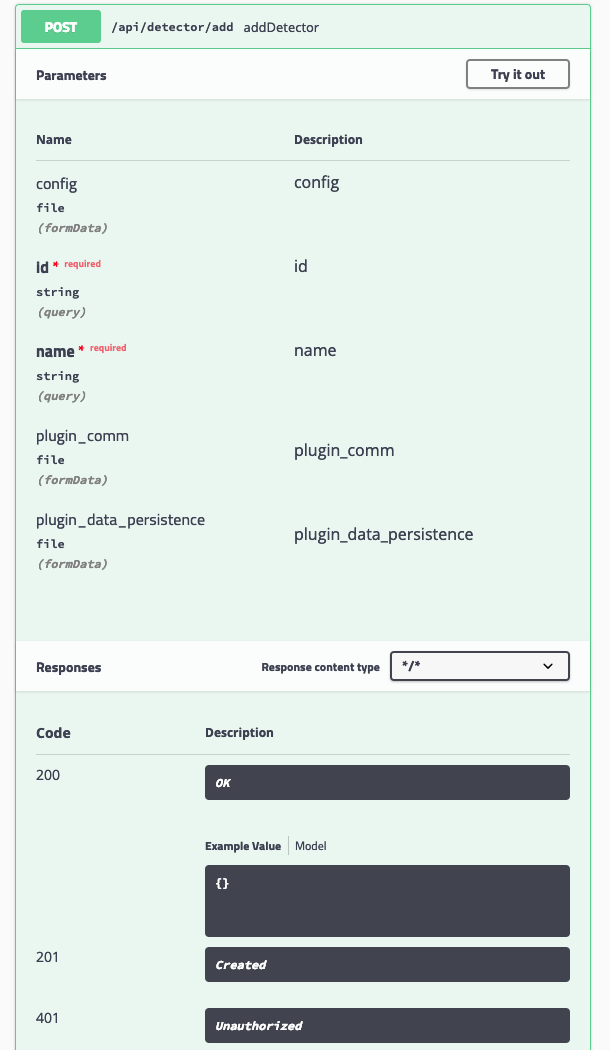
\includegraphics[width=7.0cm]{figures/handler_swagger_b.png}
			\caption{Detail endpointu.}
			\label{fig:handler:swagger_a}
		\end{subfigure}
		\caption{Springfox online dokumentace handleru.}
		\label{fig:handler:swagger}
	\end{center}
\end{figure}

\subsubsection{Webové rozhraní handleru}\label{chap:handler:spring:web}
Handler poskytuje jednoduché webové rozhraní, umožňující uživateli přehled přiřazených detektorů, viz obrázek \ref{fig:handler:web}. Rozhraní je implementováno pomocí \textit{Spring Web MVC} frameworku a \textit{Thymeleaf} (Java template engine pro vytváření HTML stránek na straně serveru). Jedná se tedy o statickou stránku a pro její obnovení je potřeba její opětovné načtení (pro vygenerování nové HTML stránky na straně serveru).

Webové rozhraní je dostupné z endpointu \texttt{/detectors}. Pro jednoduchost bylo na tento endpoint přidáno přesměrování z výchozí URL adresy (např. \url{http://localhost:8082}).

\begin{figure}[h]
	\begin{center}
		\vspace*{1cm}
		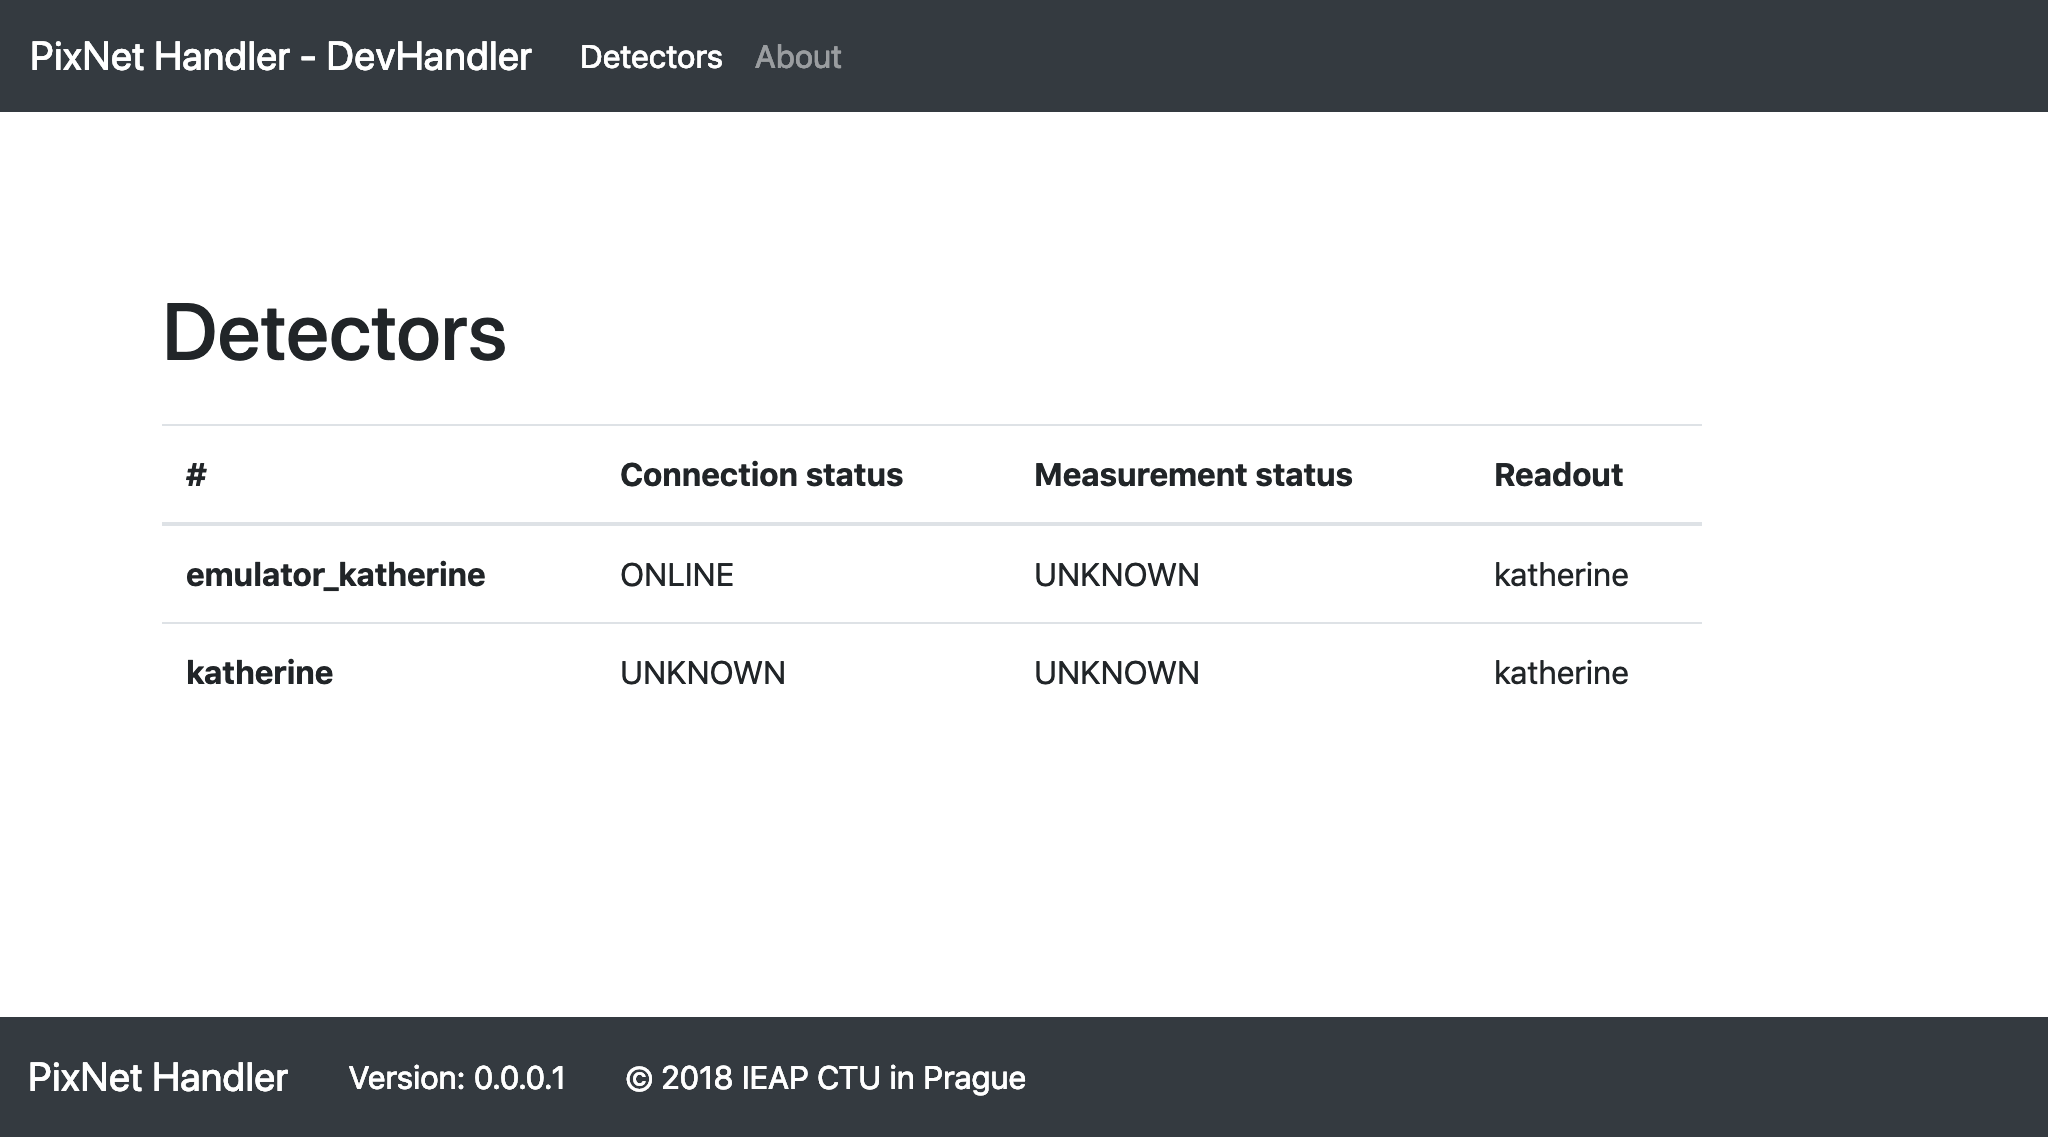
\includegraphics[width=14cm]{figures/handler_web.png}
		\caption{Screenshot webového rozhraní handleru.}
		\label{fig:handler:web}
	\end{center}
\end{figure}

%********************************************************************************
% Konfigurace a nasazení
%********************************************************************************
\section{Konfigurace a nasazení}\label{chap:handler:config}
Pro spuštění handleru je třeba mít nainstalované \texttt{JRE 8}\footnote{\textit{Java SE Runtime Environment, dostupné z\\\url{https://www.oracle.com/technetwork/java/javase/downloads}}.}, nebo vyšší.
Zkompilovanou java aplikaci je třeba spustit s argumentem \texttt{handlerConfig} obsahující cestu ke konfiguračnímu souboru (pro příklad viz zdrojový kód \ref{src:handler:config}), obsahujícího port na kterém bude aplikace naslouchat a pojmenování handleru.

Aplikaci je tedy možné spustit například takto: \mint{bash}{java -jar handler.jar handlerConfig=config.yaml}

\begin{code}[h]
  \begin{minted}[
  frame=single,
  linenos,
  breaklines
  ]{yaml}
portToListen: 8082
handlerName: Handler1
\end{minted}
\caption{\texttt{YAML} konfigurační soubor handleru.}
\label{src:handler:config}
\end{code}
\addbibresource{reference.bib}

\chapter{Vyčítací rozhraní Katherine a jeho implementace}\label{chap:katherine}
V této kapitole bude čtenář blíže seznámen s komunikačním protokolem vyčítacího rozhraní \textit{Katherine} (viz \ref{chap:detectors:readouts:katherine}) a bude zde také představena implementace komunikačního (viz \ref{src:handler:comm_intf} ) a datového (viz \ref{src:handler:data_intf}) interface, vyvinutých za účelem podpory \textit{Katherine} handlerem (viz \ref{chap:handler}). 

Pro účely vývoje a testování byl vyvinut emulátor \textit{Katherine}, který emuluje zařízení na síťové vrstvě, včetně podpory všech příkazů komunikačního protokolu relevantních k akvizici dat. Popis jeho návrhu a implementace bude také zahrnut v této kapitole.

Pro úplnost je třeba dodat, že komunikační a datový modul sdílejí stejnou podmnožinu datového modelu a část business-logiky, vázající se k manipulaci s měřenými daty. Tato společná \textit{code-base} je implementována v rámci separátního modulu, na kterém jsou závislé oba výše zmíněné moduly. Toto řešení umožňuje použití stejné vnitřní reprezentace dat, bez nutnosti jejich serializace a deserializace, což má pozitivní vliv na výkonost systému. Nutnou podmínkou ale je, aby oba moduly byly do systému zavedeny pomocí stejného \texttt{ClassLoader} objektu (z důvodu kompatibility přenášených model objektů). Tento mechanizmus je ale už implementován v handleru.

%********************************************************************************
% Komunikační protokol
%********************************************************************************
\section{Komunikační protokol}\label{chap:katherine:protocol}
Jak již bylo vysvětleno v kapitole \ref{chap:detectors:readouts:katherine:comm}, \textit{Katherine} podporuje dva provozní módy -- autonomní a manuální. Tato práce se zabývá pouze použitím manuálního módu, který umožňuje plnohodnotné řízení detektoru a umožňuje (ve srovnání s autonomním módem) efektivněji přenášet naměřená data, díky čemuž je možné maximalizovat tok výstupních dat detektoru.

Komunikace v rámci manuálního módu je založena na proprietárním komunikačním protokolu, který bude popsán v této podkapitole. Klientská část tohoto protokolu je implementována v komunikačním modulu handleru (viz \ref{chap:katherine:comm}) a jeho serverová část v \textit{Katherine} emulátoru (viz \ref{chap:katherine:emulator}).

Protokol je založen na posílání \texttt{UDP} datagramů pomocí dvou socketů\footnote{Označení pro koncový bod obousměrné komunikace mezi počítačovými programy v rámci počítačové sítě.} -- jednoho pro řídící příkazy a druhého pro měřená data. Využití \texttt{UDP} se nabízí především z důvodu implementovaného nepotvrzovaného spojení (na rozdíl od \texttt{TCP}), takže v případě špatného spojení nedochází k zahlcení a je možné dosáhnout většího datového toku. V dalších fázích vývoje je plánován přechod na \texttt{TCP} protokol pro řídící socket, protože objem jeho prostřednictvím přenášených dat je zanedbatelný a potvrzované doručení řídících příkazů by nemuselo být ošetřováno aplikační vrstvou.

%********************************************************************************
% Komunikační protokol -- Řídící příkazy
%********************************************************************************
\subsection{Řídící příkazy}\label{chap:katherine:protocol:control_commands}
Každý řídící příkaz je vždy inicializován klientem -- klient pošle 8-bytový datagram na předem definovaný komunikační port \textit{Katherine}, jehož struktura je znázorněna na obr. \ref{fig:katherine:protocol:comm_packet:request} a server (resp. \textit{Katherine}) vždy pošle odpověď ve formě datagramu (viz \ref{fig:katherine:protocol:comm_packet:response}), nebo jiných dat dle specifikace příkazu, na port klienta, ze kterého spojení bylo inicializováno\footnote{Doplnění této funkcionality bylo vyžádáno až v průběhu implementace komunikačního modulu a během psaní této práce je ještě ve fázi testování. V současné produkční verzi firmware \textit{Katherine} tedy posílá response datagram na staticky konfigurovaný port, což pro operování více \textit{Katherine} o stejné statické konfiguraci z jednoho handleru znamená konflikt portů.}. Response některých příkazů je jen potvrzení (tzv. \textit{Acknowledge}) ve formě ID příkazu a daty $0x00000000$ (dále jen ACQ). Bytové pořadí pro všechny datagramy je \textit{BigEndian}\footnote{Název pro označení endianity (bytového pořadí), kde na paměťové místo s nejnižší adresou je uložen nejvíce významný byte (MSB).}.

\begin{figure}[h]
	\begin{center}
		\begin{subfigure}{7.0cm}            
            \begin{bytefield}[endianness=big,bitwidth=0.25em]{64}
                \bitheader{63,48} \\
                \bitbox{16}{\textbf{ID}} & \bitbox{48}{Requst data (\unit{6}{B})}
            \end{bytefield}
			\caption{Request.}
			\label{fig:katherine:protocol:comm_packet:request}
		\end{subfigure}
		\hspace{0.1cm}
		\begin{subfigure}{7.0cm}            
            \begin{bytefield}[endianness=big,bitwidth=0.25em]{64}
                \bitheader{63,48} \\
                \bitbox{16}{\textbf{ID}} & \bitbox{48}{Response data (\unit{6}{B})}
            \end{bytefield}
			\caption{Response.}
			\label{fig:katherine:protocol:comm_packet:response}
		\end{subfigure}
	\end{center}
	\caption{Struktura řídícího datagramu.}
	\label{fig:katherine:protocol:comm_packet}
\end{figure}

Následuje výčet všech důležitých řídících příkazů, s jejich ID, názvem a stručným popisem.

\begin{description}
    \item[0x01 -- Set acq. time (LSB)] -- nastaví nejnižších 32 bitů akvizičního času v desítkách nanosekund.
    \\\textit{Request}: \texttt{data[31..0]} LSB akvizičního času.
    \\\textit{Response}: ACQ.

    \item[0x02 -- Set bias] -- nastaví \textit{bias} napětí detektoru.
    \\\textit{Request}: \texttt{data[39..32]} ID biasu, \texttt{data[31..0]} float\footnote{IEEE 754 standart pro reprezentaci čísel s plovoucí desetinou čárkou.} hodnota biasu.
    \\\textit{Response}: ACQ.
    
    \item[0x03 -- Acquisition Start] -- spuštění akvizice dat.
    \\\textit{Request}: \texttt{data[0]} akviziční mód (0 = sekvenční, 1 = data-driven).
    \\\textit{Response}: ACQ.
    
    \item[0x04 -- Internal DAC Settings] -- nastavení hodnoty DAC (digitálně analogového převodníku) detektoru. Přehled jednotlivých dat je uveden v příloze \ref{chap:app:katherine:dacs}.
    \\\textit{Request}: \texttt{data[15..0]} hodnota DAC, \texttt{data[16..31]} ID DAC pro čtení.
    \\\textit{Response}: ACQ.

    %\item[0x05 -- Seq. Readout Start] -- TODO
    
    \item[0x06 -- Acquisition Stop] -- zastaví probíhající akvizici dat (měření).
    \\\textit{Request}: prázdný.
    \\\textit{Response}: ACQ.
    
    \item[0x07 -- HW Command Start] -- spustí interní hardwarový příkaz vyčítacího rozhraní. Přehled HW příkazů je uveden v příloze \ref{chap:app:katherine:hw_commands}.
    \\\textit{Request}: \texttt{data[7..0]} ID HW příkazu.
    \\\textit{Response}: ACQ.

    \item[0x08 -- Sensor Register Setting] -- nastavení registru připojeného \textit{Timepix3} detektoru ve vyčítacím rozhraní. Přehled registrů je uveden v příloze \ref{chap:app:katherine:tpx3_registers}. Pro propsání nastavení registru do detektoru je třeba ještě vykonat interní HW příkaz s ID \textbf{0}.
    \\\textit{Request}: \texttt{data[39..32]} ID registru, \texttt{data[31..0]} hodnota registru.
    \\\textit{Response}: ACQ.
    
    \item[0x09 -- Acquisition Mode Setting] -- nastavení akvizičního módu detektoru.
    \\\textit{Request}: \texttt{data[1..0]} akviziční mód (00 = \textit{ToA \& ToT}, 01 = \textit{pouze ToA}, 10 = \textit{Event \& iTOT}), \texttt{data[7]} povolení \textit{FastToA}\footnote{LSB (bit s nejnižší hodnotou) ToA je \unit{25}{ns}, s aktivovaným FastToA je časové rozlišení zlepšeno na \unit{1.5625}{ns}} (1 = povoleno).
    \\\textit{Response}: ACQ.

    \item[0x0A -- Acquisition Time Setting -- MSB] -- nastaví nejvyšších 32 bitů akvizičního času v desítkách nanosekund.
    \\\textit{Request}: \texttt{data[31..0]} MSB akvizičního času.
    \\\textit{Response}: ACQ.

    \item[0x0B -- Echo Chip ID] -- vrátí ID připojeného detektoru.
    \\\textit{Request}: nic.
    \\\textit{Response}: \texttt{data[31..0]} ID detektoru.

    \item[0x0C -- Get Bias Voltage] -- změří a vrátí bias napětí detektoru.
    \\\textit{Request}: \texttt{data[39..32]} ID biasu.
    \\\textit{Response}: \texttt{data[31..0]} float hodnotu biasu detektoru.

    %\item[0x0D -- Get ADC Voltage] -- 
    %\item[0x0E -- Get Back Read Register] -- 

    \item[0x0F -- Internal DAC Scan] -- naměří a vrátí hodnotu DAC.
    \\\textit{Request}: \texttt{data[7..0]} ID DAC (viz \ref{tab:app:dacs}).
    \\\textit{Response}: \texttt{data[31..0]} float hodnota napětí analogového výstupu převodníku.

    %\item[0x10 -- Set Pixel Config] -- nastaví konfiguraci jednotlivých pixelů detektoru. V příloze \ref{chap:app:katherine:pix_config} je příklad převodu z formátu \texttt{BMC}\footnote{Z angl. \textit{Binary Matrix Configuration}, standardizovaný formát pro konfiguraci pixelů detektorů rodiny Medipix.} do formátu vyžadovaného \textit{Katherine} rozhraním.
    %\\\textit{Request}: nejprve je poslán příkaz z prázdnými daty. Poté \textit{Katherine} očekává 65536 bytů s konfigurací pixelů.
    %\\\textit{Response}: ACQ.

    %\item[0x11 -- Get Pixel Config ] -- příkaz vyčte a vrátí konfiguraci pixelů detektoru.
    %\\\textit{Request}: nic.
    %\\\textit{Response}: posloupnost 65536 bytů s konfigurací pixelů.

    \item[0x12 -- Set All Pixel Config] -- nastaví konfiguraci jednotlivých pixelů detektoru. V příloze \ref{chap:app:katherine:pix_config} je příklad převodu z formátu \texttt{BMC}\footnote{Z angl. \textit{Binary Matrix Configuration}, standardizovaný formát pro konfiguraci pixelů detektorů rodiny Medipix.} do formátu vyžadovaného \textit{Katherine} rozhraním.
    \\\textit{Request}: nejprve je poslán příkaz z prázdnými daty. Poté \textit{Katherine} očekává 65536 bytů s konfigurací pixelů.
    \\\textit{Response}: ACQ.

    \item[0x13 -- Number of Frames Setting] -- nastaví počet snímků, které se naměří, je-li akvizice dat spuštěna v \textit{frame-based} módu (viz \ref{chap:detectors:operation_modes}).
    \textit{Request}: \texttt{data[31..0]} počet snímků.
    \textit{Response}: ACQ.

    \item[0x14 -- Get All DAC Scan] -- vrátí sekvenci 22 naměřených hodnot DAC, seřazených dle čtecího ID DAC (viz \ref{chap:app:katherine:dacs}).
    \\\textit{Request}: nic.
    \\\textit{Response}: 22 response datagramů, kde \texttt{data[31..0]} je float hodnota napětí analogového výstupu převodníku.

    \item[0x15 -- Get HW/Readout Temperature] -- naměří a vrátí teplotu vyčítacího rozhraní.
    \\\textit{Request}: nic.
    \\\textit{Response}: \texttt{data[31..0]} teplota (v °C, float).

    %\item[0x16 -- LED settings] -- 
    
    \item[0x17 -- Get Readout Status] -- vrátí informace o své HW a FW konfiguraci.
    \\\textit{Request}: nic.
    \\\textit{Response}: \texttt{data[7..0]} typ hardware ($0x1$ pro \textit{Katherine} ethernet readout),\\\texttt{data[15..8]} verze HW revize, \texttt{data[31..16]} sériové číslo HW, \texttt{data[47..32]} verze FW.

    \item[0x18 -- Get Communication Status] -- vrátí stav komunikace mezi vyčítacím rozhraním a detektorem.
    \\\textit{Request}: nic.
    \\\textit{Response}: \texttt{data[7..0]} maska komunikačních kanálů, \texttt{data[15..8]} aktuální maximální datový tok mezi vyčítacím rozhraním a detektorem (float, po vynásobení této hodnoty 5 je získána výsledná hodnota v Mb/s), \texttt{data[16]} flag připojení detektoru (1 = přípojen).

    \item[0x19 -- Get Sensor Temperature] -- naměří a vrátí teplotu senzoru připojeného detektoru.
    \\\textit{Request}: nic.
    \\\textit{Response}: \texttt{data[31..0]} teplota (v °C, float).

    \item[0x20 -- Digital Test] -- provede test digitální části detektoru a vrátí výsledek. Je-li výsledek roven 64, pak test proběhl v pořádku.
    \\\textit{Request}: nic.
    \\\textit{Response}: \texttt{data[7..0]} výsledek testu.

    \item[0x28 -- ToA Calibration Setup] -- zapnutí/vypnutí \textit{ToA offset korekce} (viz \ref{chap:detectors:calibration:toa_correction}).
    \\\textit{Request}: \texttt{data[0]} zapnutí \textit{ToA offset korekce} (1 = zapnuto).
    \\\textit{Response}: ACQ.

\end{description}

%********************************************************************************
% Komunikační protokol -- Struktura měřených dat
%********************************************************************************
\subsection{Struktura měřených dat}\label{chap:katherine:protocol:measure_data_structure}
Přenos měřených dat je realizován proudem datagramů ze serveru (vyčítací rozhraní) do klienta (např. handler). Data jsou posílána na předem definovaný port, uložený ve statické konfiguraci \textit{Katherine}\footnote{V době psaní této práce probíhal vývoj podpory pro dynamické nastavování klientského portu (přidáním nového příkazu do řídící části komunikačního protokolu).}. Každý datagram má délku 6 bytů a jeho struktura je znázorněna na obr. \ref{fig:katherine:protocol:data_packet}. Přehled typů datagramů, vč. jejich významu a obsažených dat, je uveden v tabulce \ref{tab:katherine:protocol:data_packet_header}.

\begin{figure}[h]
	\begin{center}
        \begin{bytefield}[endianness=big,bitwidth=0.7em]{48}
            \bitheader{47,0} \\
            \bitbox{12}{\textbf{Hlavička} 47..44} & \bitbox{36}{\textbf{Data} 43..0}
        \end{bytefield}
	\end{center}
	\caption{Struktura datagramu s měřenými daty.}
	\label{fig:katherine:protocol:data_packet}
\end{figure}

\begin{table}[h]
	\begin{center}
		\begin{tabular}{|c|l|l|}
			\hline
            \textbf{Hlavička} & \textbf{Název} & \textbf{Data} \\
			\hline
            0x7 & Nový frame vytvořen & 0x0 \\
            0x4 & Měřená data & Dle konfigurace \\
            0x5 & ToA timestamp offset & ToA offset \\
            & (pouze pro data-driven mód) & \\
            0xC & Aktuální snímek vytvořen & Počet poslaných událostí \\
            0x8 & Frame start timestamp LSB & \unit{32}{b} LSB \\
            0x9 & Frame start timestamp MSB & \unit{16}{b} MSB \\
            0xA & Frame end timestamp LSB & \unit{32}{b} LSB \\
            0xB & Frame end timestamp MSB & \unit{16}{b} MSB \\
            0xD & Počet ztracených pixelů & \unit{44}{b} \\
            0xE & Notifikace o přerušeném měření & 0x0 \\
			\hline
		\end{tabular}
	\end{center}
    \caption{Přehled typů datagramů pro měřená data.}
    \label{tab:katherine:protocol:data_packet_header}
\end{table}

%Výsledný čas ToA (viz \ref{chap:detectors:operation_modes}) je vypočten 
Z pohledu pořadí toku jednotlivých datagramů rozlišujeme dva případy, dle nastaveného vyčítacího módu:
\begin{description}
   \item[Frame-based] -- vyčítání po snímcích (viz \ref{chap:detectors:readout})
   \begin{enumerate}
       \item Klient pošle \textit{Acquisition Start} (0x03) příkaz.
       \item Vyčítací rozhraní zahájí akvizici snímku a pošle datagram o vytvoření nového frame (hlavička 0x7).
       \item Akvizice dat probíhá po dobu zvoleného akvizičního času. Jsou-li detekovány nějaké události, pak pro každou událost je poslán datagram s měřenými daty (hlavička 0x4). V případě zaznamenání příkazu pro přerušení měření, dojde k poslání datagramu s hlavičkou 0xE a měření je ukončeno.
       \item Po ukončení akvizice aktuálního snímku (uzavření \textit{shutteru}) readout pošle timestamp začátku a konce akvizice dat (datagramy s hlavičkami 0x8, 0x9, 0xA a 0xB).
       \item Je poslán datagram s informací o počtu ztracených pixelů (hlavička 0xD) a ukončení aktuálního snímku (hlavička 0xC).
       \item Je-li počet aktuálně pořízených snímků nižší, než celkový počet snímků (nastavený řídícím příkazem 0x13), pak měření pokračuje bodem 2, v opačném případě měření končí.
   \end{enumerate}
   \item[Data-driven] -- režim kontinuální vyčítání dat (viz \ref{chap:detectors:readout})
   \begin{enumerate}
    \item Klient pošle \textit{Acquisition Start} (0x03) příkaz.
    \item Vyčítací rozhraní zahájí akvizici dat (resp. jednoho snímku) a pošle datagram o vytvoření nového frame (hlavička 0x7).
    \item Akvizice dat probíhá po dobu zvoleného akvizičního času. Jsou-li detekovány nějaké události, pak pro každou událost je poslán datagram s měřenými daty (hlavička 0x4). V případě zaznamenání příkazu pro přerušení měření, dojde k poslání datagramu s hlavičkou 0xE a měření je ukončeno.
    \item Po ukončení akvizice aktuálního snímku (uzavření \textit{shutteru}) readout pošle timestamp začátku a konce akvizice dat (datagramy s hlavičkami 0x8, 0x9, 0xA a 0xB).
    \item Je poslán datagram s informací o počtu ztracených pixelů (hlavička 0xD) a ukončení aktuálního snímku (hlavička 0xC).
    \item Měření je ukončeno.
\end{enumerate}
\end{description}

Tabulka \ref{tab:katherine:protocol:measurement_data_structure} znázorňuje formát datagramu s měřenými daty, dle použitého nastavení vyčítacího rozhraní.

\begin{table}[h!]
    \begin{center}
        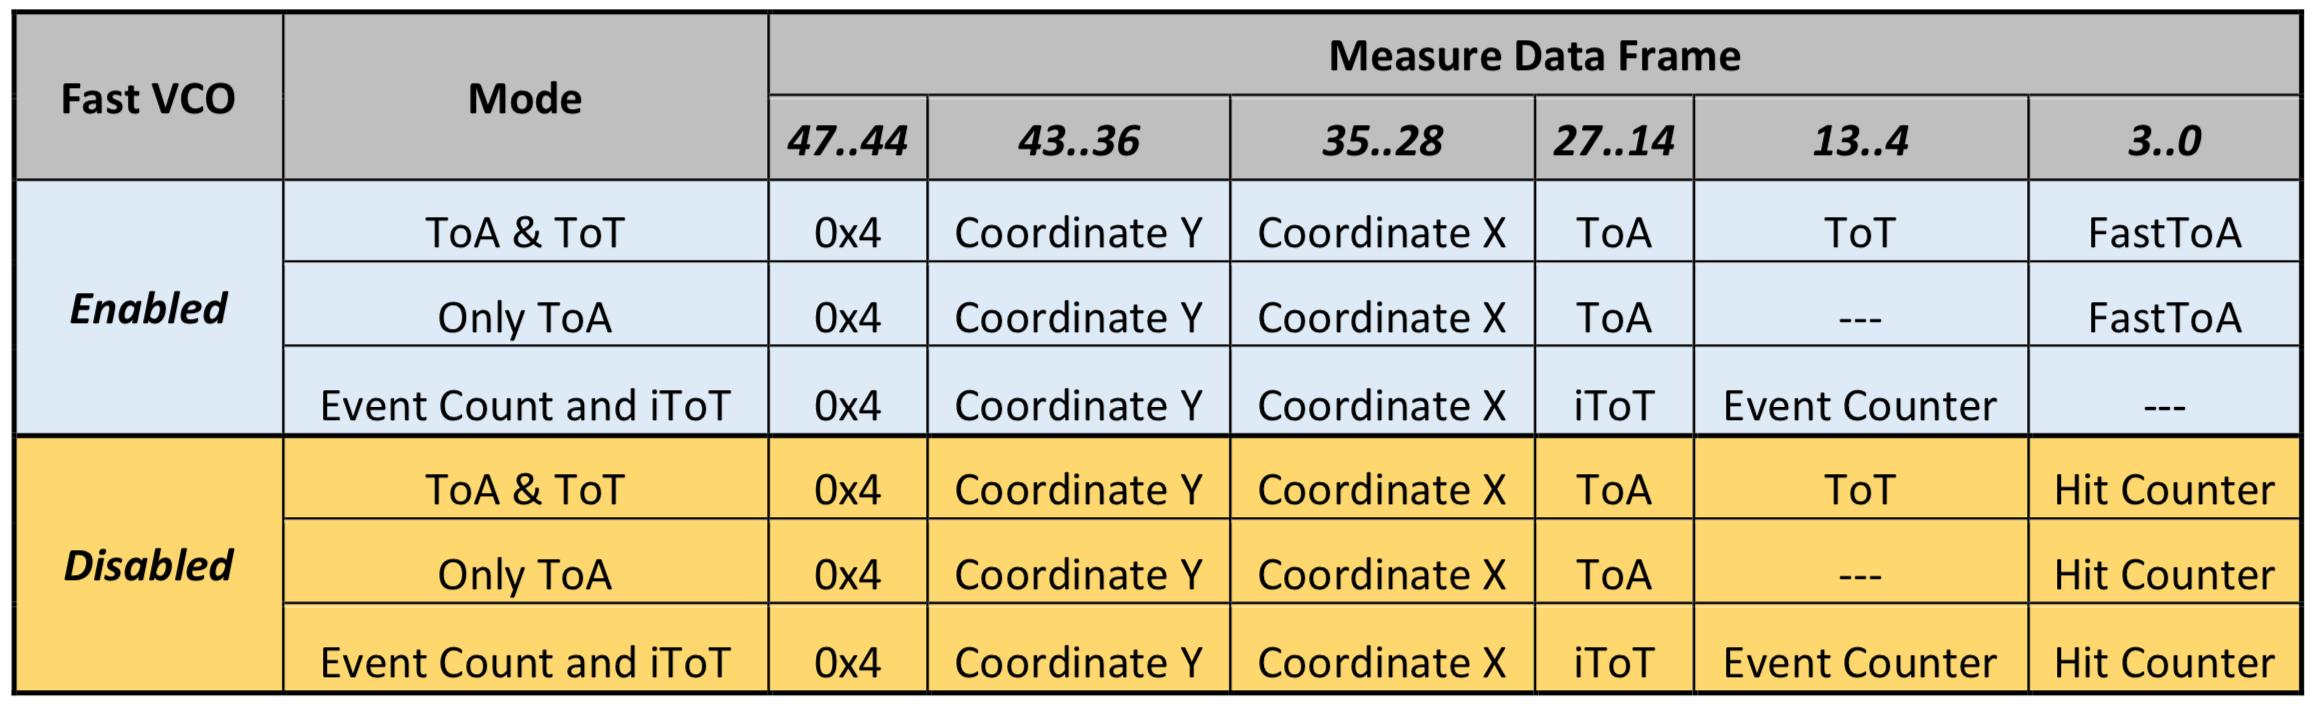
\includegraphics[width=14cm]{figures/katherine_pixel_measurement_data.png}
        \caption{Struktura měřených dat \cite{katherine_docs}.}
        \label{tab:katherine:protocol:measurement_data_structure}
    \end{center}
\end{table}

%********************************************************************************
% Komunikační modul
%********************************************************************************
\section{Komunikační modul}\label{chap:katherine:comm}
Pro účely řízení komunikačního rozhraní \textit{Katherine} a vyčítání měřených dat byl implementován komunikační modul, který bude popsán v této podkapitole. Aby bylo možné integrovat modul do systému, musí obsahovat implementaci komunikačního interface (viz \ref{chap:handler:detector_layer:commIntf}), které musí být v manifestu zkompilovaného \texttt{jar} archívu explicitně uvedeno (viz \ref{chap:handler:detector_layer:module_init}).

Na obrázku \ref{fig:katherine:comm:arch} je přehled vrstev softwarové architektury komunikačního modulu, které budou dále popsány v následujících podkapitolách.

\begin{figure}[h]
	\begin{center}
		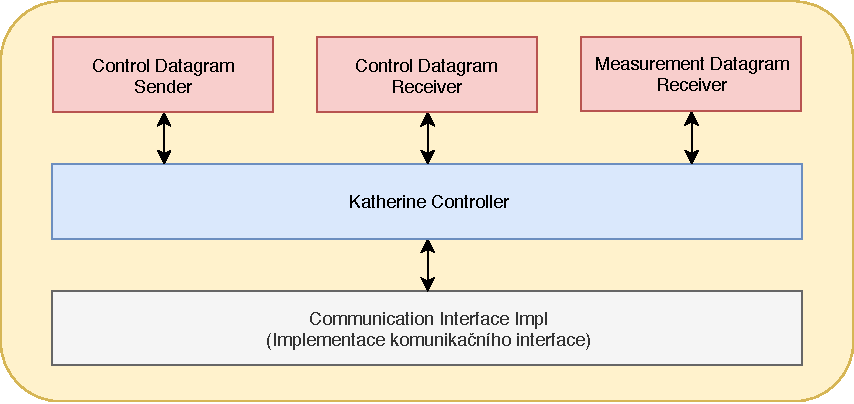
\includegraphics[width=14cm]{figures/katherine_comm_arch.pdf}
		\caption{Softwarová architektura komunikačního modulu, implementujícího komunikační interface.}
		\label{fig:katherine:comm:arch}
	\end{center}
\end{figure}

\subsection{Implementace komunikačního interface}
Tato vrstva slouží jako tzv. fasáda\footnote{Návrhový vzor fasáda (\textit{Facade Pattern}) -- použití pro poskytování zjednodušeného interface pro komplexní části kódu (analogie s pojmem fasáda, známém z architektury).} Katherine kontroléru. Implementace komunikačního interface implementuje všechny jeho metody, vč. poskytování přehledu a podpory vykonávání \textit{ValueCommands} a \textit{ExecutionCommands} (pro jejich definici viz soubor \texttt{detector\_model.json} na přiloženém CD, viz příloha \ref{chap:app:cd}), navazování spojení s detektorem, nahrávání konfigurace apod.

Po zavedení modulu je vytvořena fronta měřených dat, která je přejatá handlerem.

Připojením detektoru vzniká instance Katherine kontroléru dle předané konfigurace. Při odpojení detektoru je kontrolér notifikován, aby mohl uvolnit svoje prostředky (např. uzavřít síťové spojení) a poté je odstraněn.

\subsection{Katherine kontrolér}
Tato vrstva udržuje spojení s detektorem a implementuje všechny potřebné řídící příkazy detektoru.

Odesílání řídících příkazů je realizováno pomocí komponenty \texttt{Control Datagram Sender} (viz obr. \ref{fig:katherine:comm:arch}), který implementuje asynchronní frontu datagramů. Fronta je asynchronně zpracovávána nezávislým vláknem, které datagramy z fronty odesílá na řídící port \textit{Katherine}.

O příjem dat z řídícího socketu se stará komponenta \texttt{Control Datagram Receiver}, která v separátním vlákně přijímá příchozí data. Každý příchozí datagram (8-bytový vektor) je zpracován a přidán do fronty příchozích řídících dat. Komponenta také implementuje blokující metodu pro přijetí dat, která dle zadaného ID příkazu a maximální doby čekání (tzv. \textit{timeout}) hledá požadovanou odpověď ve frontě dat.

Příklad použití obou komponent zmíněných výše je ve zdrojovém kódu \ref{src:katherine:comm:example_get_bias}. Příklad demonstruje vyčtení biasu z detektoru. Nejprve je pomocí \texttt{Control Datagram Sender} odeslán řídící příkaz s ID 0x0C (řádek 3 až 7) a následně pomocí \texttt{Control Datagram Receiver}, resp. pomocí jeho blokující metody popsané výše, je zachycena odpověď, ze které je vyčtena požadovaná hodnota napětí. Jestli se odpověď nepodaří přijmout ve zvoleném timeoutu, je vygenerována výjimka, která musí být vyššími vrstvami programu ošetřena.

\begin{code}[h]
    \begin{minted}[
      frame=single,
        linenos,
        breaklines
      ]{Kotlin}
@Throws(DetectorException::class)
fun getBias(): Float {
    packetSender.send(
        PacketBuilder.builder()
            .commandID(KatherineValueCommands.BIAS.getterCommandId)
            .build()
    )

    val packet = packetReceiver.pollPacketFromQueue(
        KatherineValueCommands.BIAS.getterCommandId,
        RESPONSE_TIMEOUT
    )
    return packet.floatValue
}
    \end{minted}
    \caption{Příklad implementace řídícího příkazu \textit{Katherine} pro vyčtení biasu pomocí komponent \texttt{Control Datagram Sender} a \texttt{Control Datagram Receiver}.}
    \label{src:katherine:comm:example_get_bias}
\end{code}

Poslední komponentou je \texttt{Measurement Datagram Receiver}, který ve svém separátním vlákně přijímá příchozí datagramy na socketu pro detektorem měřená data, jejichž struktura už byla popsána v \ref{chap:katherine:protocol:measure_data_structure}. Každá příchozí událost je zpracována (identifikace hlavičky apod.) a vložena do fronty měřených dat, která je zpracovávána datovým modulem.

%********************************************************************************
% Datový modul
%********************************************************************************
\section{Datový modul}\label{chap:katherine:data}
Datový modul implementuje \texttt{DataPersistence} interface (viz \ref{chap:handler:detector_layer:dataIntf}). Po jeho zavedení do systému je mu handlerem předána fronta dat, kterou po spuštění začne zpracovávat.

Fronta dat obsahuje objekty, které jsou potomky objektu \texttt{AbstractDataFrame} (který je součástí modelu poskytovaných knihoven). V rámci modulu se společnou \textit{code-base} \textit{Katherine} modulů (viz úvod kapitoly \ref{chap:katherine}) byly implementovány tyto třídy, které jsou potomky třídy \texttt{AbstractDataFrame}:
\begin{description}
    \item[\texttt{DataFrame}] -- třída obsahující jednu událost, přenesenou datovým socketem z \textit{Katherine} rozhraní. Objekt obsahuje dekódovanou hlavičku a vlastní data, dle typu datagramu -- viz tabulka \ref{tab:katherine:protocol:data_packet_header}.
    \item[\texttt{ControlFrame}] -- obsahuje informaci generovanou komunikačním modulem, např. o začátku nebo ukončení akvizice apod.
    \item[\texttt{AcqConfigurationFrame}] -- instance tohoto objektu je poslána komunikačním modulem na začátku akvizice dat a obsahuje informace o stavu a konfiguraci detektoru (např. bias, vyčítací mód, teploty apod.).
\end{description}  

Výstupem datového modulu jsou soubory s jednotlivými měřeními ve formátu \texttt{ASCII}, které jsou ukládány do zvoleného adresáře dle konfigurace. Příklad obsahu takového souboru je uveden v příloze \ref{chap:app:katherine:data_example}. Všechny časové údaje jsou v \texttt{UTC} čase. Formát pojmenovávání souborů je \texttt{název\_detektoru\_yyyy\_MM\_dd-HH\_mm\_ss.txt}.

Rovněž byla implementována varianta datového modulu, který ukládá pořízená data do \textit{MongoDB} databáze (viz \ref{chap:arch:technologie:mongodb}).

%********************************************************************************
% Katherine emulátor
%********************************************************************************
\section{Katherine emulátor}\label{chap:katherine:emulator}
Pro účely vývoje a testování byl vyvinut emulátor, které emuluje funkci \textit{Katherine} vyčítacího rozhraním s připojeným \textit{Timepix3} (viz \ref{chap:detectors:medipix_overview:timepix3}) detektorem na síťové vrstvě. Byla implementována podpora pro všechny řídící příkazy uvedené v \ref{chap:katherine:protocol:control_commands}, které jsou relevantní k akvizici dat (tj. např. akviziční čas, akviziční mód, vyčítací mód, bias, počet snímků apod.) a také příkazy pro měření teplot, vyčítání ID senzoru, či provádění testu digitální částí detektoru. Emulátor rovněž podporuje všechny datagramy pro přenos měřených dat (viz \ref{chap:katherine:protocol:measure_data_structure}).

Emulátor byl vyvinut v jazyce \texttt{Java}, resp. \texttt{Kotlin} (viz \ref{chap:arch:technologie:kotlin}).

\subsection{Softwarová architektura}
Na obrázku \ref{fig:katherine:emulator:arch} jsou znázorněny jednotlivé komponenty emulátoru. Základním prvkem je jeho jádro (na obr. \ref{fig:katherine:emulator:arch} jako \textit{emulator core}), které je vytvořeno po spuštění emulátoru. Společně s jádrem je vytvořen také \textit{Control Datagram Receiver}, který přijímá příchozí datagramy na komunikačním socketu detektoru. Příchozí řídící datagram je dále zpracován dle jeho hlavičky a klientovi je odeslána příslušná odpověď.

\begin{figure}[h]
	\begin{center}
		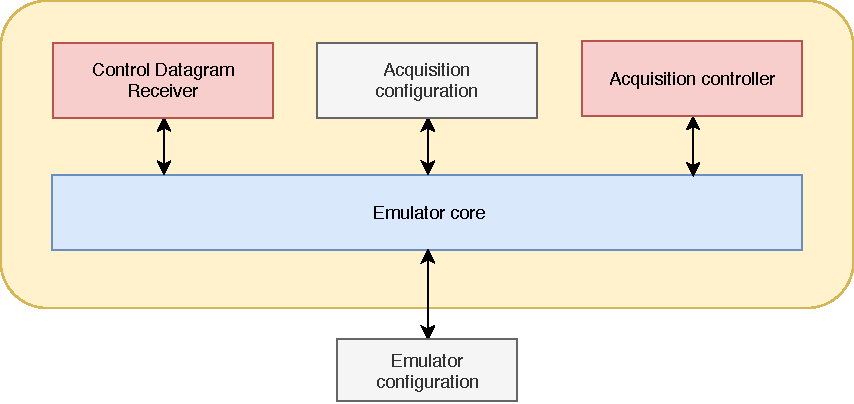
\includegraphics[width=14cm]{figures/katherine_emulator_arch.pdf}
		\caption{Softwarová architektura \textit{Katherine} emulátoru.}
		\label{fig:katherine:emulator:arch}
	\end{center}
\end{figure}

Z pohledu zpracování je možné příkazy rozdělit do tří kategorií:
\begin{description}
    \item[Nastavení akvizičních parametrů] -- do této skupiny spadají všechny příkazy, které nastavují, nebo vracejí konfigurační parametry detektoru, jako je akviziční čas, bias, akviziční a vyčítací mód apod.
    \item[Řízení akvizice] -- do této kategorie patří příkazy \textit{Acquisition Start} (0x03) a \textit{Acquisition Stop} (0x06). Po spuštění akvizice je vytvořena instance \texttt{Acquisition Controller}, který dle konfigurace začne generovat události a posílat je datovým socketem klientovi.
    
    Příkaz \textit{Acquisition Stop} pak přeruší probíhající akvizici.
    \item[Ostatní] -- do této kategorie spadají ostatní příkazy, které nebyly zahrnuty v předchozích kategoriích (např. pro měření teploty, čtení \textit{chip id}, verze FW apod.).
\end{description}

Některé příkazy nebyly implementovány, protože emulace jejich funkce není triviální a je nad rámec požadované funkcionality (jsou to např. příkazy pro nastavování hodnot DAC, registrů apod.). Odpovědí na tyto příkazy bude vždy ACQ (viz \ref{chap:katherine:protocol:control_commands}).

\subsection{Konfigurace a nasazení}
Pro spuštění emulátoru vyčítacího rozhraní \textit{Katherine} je třeba mít nainstalované \texttt{JRE 8}\footnote{\textit{Java SE Runtime Environment, dostupné z\\\url{https://www.oracle.com/technetwork/java/javase/downloads}}.}, nebo vyšší.
Zkompilovanou Java aplikaci je třeba spustit s argumentem cesty ke konfiguračnímu souboru (pro příklad viz zdrojový kód \ref{src:emulator:config}). Konfigurační soubor obsahuje číslo portu, na které bude emulátor naslouchat pro řídící příkazy (\texttt{portCommands}), číslo portu a adresu pro odesílání měřených dat (\textit{portCommands} a \texttt{hots}) a parametr udávající průměrný počet události, které budou v rámci jedné akvizice vygenerovány.

Aplikaci je tedy možné spustit například takto: \mint{bash}{java -jar emulator.jar config.yaml}

\begin{code}[h]
  \begin{minted}[
  frame=single,
  linenos,
  breaklines
  ]{yaml}
portCommands: 1555
portData: 1556
host: 127.0.0.1
avgNumberOfEventsPerAcq: 10
\end{minted}
\caption{\texttt{YAML} konfigurační soubor emulátoru vyčítacího rozhraní \textit{Katherine}.}
\label{src:emulator:config}
\end{code}
\addbibresource{reference.bib}

\chapter{Master}\label{chap:master}
V této kapitole bude čtenář podrobněji seznámen s masterem -- centrálním řídícím prvkem systému Pixnet. Hlavním úkolem masteru je řízení handlerů (viz \ref{chap:handler}), persistence konfigurace a poskytování REST API pro své řízení. Primárním konzumentem API je webová frontend aplikace, poskytující uživatelské rozhraní pro řízení systémů jeho operátorem, pomocí poskytovaného API může být ale řízení systému integrováno i do systémů třetích stran\footnote{Např. DCS v CERN, jak již bylo popsáno v kapitole \ref{chap:arch:hw}}.

Tato komponenta se skládá ze dvou nezávislých částí -- backendového serveru (\ref{chap:master:backend}) frontendového webového klienta (\ref{chap:master:frontend}).

%********************************************************************************
% Backend
%********************************************************************************
\section{Backend}\label{chap:master:backend}
Backendová aplikace mastera, podobně jako handlera, byla implementována pomocí Spring Boot frameworku (viz \ref{chap:arch:technologie:spring}) a obsahuje embedovaný webový server \texttt{Tomcat}. Aplikace komunikuje s handlery, jejichž prostřednictvím řídí jim přiřazené detektory.

\subsection{Softwarová architektura}\label{chap:master:backend:sw_arch}
Na obrázku \ref{fig:master:arch} je znázorněna softwarová architektura backendové aplikace mastera, rozdělená do několika vrstev, které budou v následujících podkapitolách blíže vysvětleny.

\begin{figure}[h]
	\begin{center}
		\vspace*{0.4cm}
		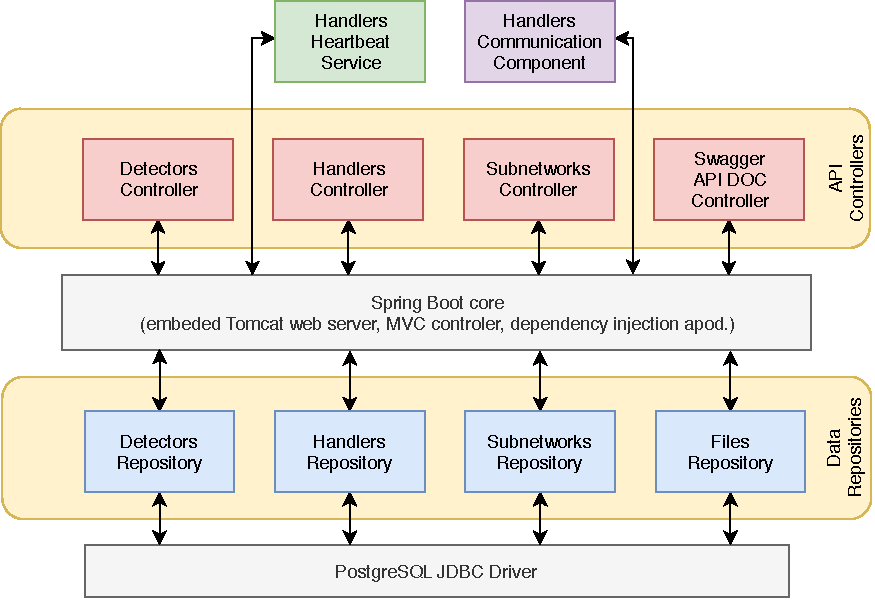
\includegraphics[width=14cm]{figures/master_arch.pdf}
		\caption{Pixnet -- master: softwarová architektura s vrstvami pro (i) persistenci konfiguraci s stavu systému (\textit{Data Repositories}), (ii) poskytování API (\textit{API controllers}),(iii) komponentu pro komunikaci s handlery (\textit{Handlers Communication Component}) a (iv) službu pro pravidelnou aktualizaci stavu handlerů (\textit{Handler Heartbeat Service}).}
		\label{fig:master:arch}
	\end{center}
\end{figure}

\subsubsection{Vrstva pro persistenci konfigurace a stavu systému}
Tato vrstva je zodpovědná za komunikaci s \textit{PostgreSQL} databází (viz \ref{chap:arch:technologie:postgresql}) pomocí \textit{PostgreSQL} \texttt{JDBC}\footnote{Z angl. \textit{Java Database Connectivity} -- API pro programovací jazyk Java, definující přístup klienta k databázi.} ovladače. Pro mapování jednotlivých entit (resp. Java objektů, tzv. \texttt{ORM}\footnote{Z angl. \textit{Object-relational mapping} -- objektově-relační mapování.}) byl implementován framework \textit{Hibernate}.

Vrstva poskytuje repozitáře (viz obr. \ref{fig:master:arch}) pro dotazy nad uloženými daty a pro jejich modifikaci. Rovněž je zodpovědná za automatické vytváření a aktualizaci databázového schématu, připojené databáze. Návrh schématu bude popsán v \ref{chap:master:backend:db}.

V databázi jsou společně se záznamem detektoru uloženy také jeho moduly (resp. implementace komunikačního a datového interface).

\subsubsection{Komponenta pro komunikaci s handlery}
Komponenta poskytuje metody pro komunikaci s handlery pomocí jejich API, popsaném v \ref{tab:handler:api_detectors}. Umožňuje přiřazování detektorů jednotlivým handlerům, navazování spojení s detektory, zjišťování jejich stavu a funkcionality (vč. seznamů podporovaných příkazů), vykonávání jednotlivých příkazů, nahrávání souborů apod.

\subsubsection{Vrstva s API kontroléry}\label{chap:master:backend:sw_arch:api}
Tato vrstva se sestává z REST API kontrolérů pro poskytování API metod pro řízení mastera. Těmito kontroléry jsou:
\begin{description}
    \item[\texttt{Subnetworks Controller}] -- poskytuje CRUD\footnote{Z angl. \textit{Create Read Update and Delete}, operace pro vytváření, čtení, aktualizaci a odstranění.} operace nad entitou podsítí (viz \ref{chap:arch:hw}). Pro přehled endpointů viz tabulka \ref{tab:master:api_subnetworks}.

    \begin{table}[h!]
        \begin{center}
            \begin{tabular}{|c|c|l|}
                \hline
          \textbf{HTTP} & & \\
          \textbf{Metoda} & \textbf{Endpoint} & \textbf{Popis} \\
            \hline
            POST & \texttt{/add} & Přidá novou podsíť \\
            GET & \texttt{/getAll} & Vrátí seznam všech podsítí \\
            DELETE & \texttt{/deleteAll} & Odstraní všechny podsítě \\
            DELETE & \texttt{/deleteById} & Odstraní podsíť podle zadaného ID \\
            \hline
            \end{tabular}
        \end{center}
        \caption{Endpointy komponenty \textit{Subnetworks Controller} (všechny endpointy mají prefix \texttt{/api/subnetwork}).}
        \label{tab:master:api_subnetworks}
    \end{table}

    \item[\texttt{Handlers Controller}] -- poskytuje CRUD operace nad entitou handlerů. Pro přehled endpointů viz tabulka \ref{tab:master:api_handlers}.

    \begin{table}[h!]
        \begin{center}
            \begin{tabular}{|c|c|l|}
                \hline
          \textbf{HTTP} & & \\
          \textbf{Metoda} & \textbf{Endpoint} & \textbf{Popis} \\
            \hline
            POST & \texttt{/add} & Přidá nový handler \\
            GET & \texttt{/getAll} & Vrátí seznam všech handlerů \\
            DELETE & \texttt{/deleteAll} & Odstraní všechny handlery \\
            DELETE & (pouze prefix) & Odstraní handler podle zadaného ID \\
            \hline
            \end{tabular}
        \end{center}
        \caption{Endpointy komponenty \textit{Handlers Controller} (všechny endpointy mají prefix \texttt{/api/handler}).}
        \label{tab:master:api_handlers}
    \end{table}

    \item[\texttt{Detectors Controller}] -- kromě poskytování CRUD operací nad entitou detektorů také poskytuje metody pro přiřazování detektorů handlerům, navazování spojení s detektory, vykonávání jejich příkazů (viz \textit{ValueCommands} a \textit{ExecutionCommands}, \ref{chap:handler:detector_layer:commIntf}). Pro přehled endpointů viz tabulka \ref{tab:master:api_detectors}.

    \begin{table}[h!]
        \begin{center}
            \begin{tabular}{|c|c|l|}
                \hline
          \textbf{HTTP} & & \\
          \textbf{Metoda} & \textbf{Endpoint} & \textbf{Popis} \\
            \hline
            POST & \texttt{/add} & Přidá nový detektor \\
            GET & \texttt{/getAll} & Vrátí seznam všech detektorů \\
            GET & \texttt{/getById} & Vrátí jeden detektor \\
            GET & \texttt{/getDetailById} & Vrátí detail jednoho detektoru \\
            DELETE & (pouze prefix) & Odstraní detektor podle zadaného ID \\
            POST & \texttt{/bindToHandler} & Přiřadí detektor handleru \\
            POST & \texttt{/unbindFromHandler} & Odebere detektor handleru \\
            POST & \texttt{/connect} & Naváže spojení mezi handlerem a detektorem \\
            POST & \texttt{/disconnect} & Ukončí spojení mezi handlerem a detektorem \\
            POST & \texttt{/executeValueCommand} & Vykoná \texttt{ValueCommand} detektoru \\
            POST & \texttt{/executeExecutionCommand} & Vykoná \texttt{ExecutionCommand} detektoru \\
            POST & \texttt{/uploadFile} & Nahraje soubor do detektoru \\
            \hline
            \end{tabular}
        \end{center}
        \caption{Endpointy komponenty \textit{Detectors Controller} (všechny endpointy mají prefix \texttt{/api/detector}).}
        \label{tab:master:api_detectors}
    \end{table}    

    \item[\texttt{Swagger API DOC Controller}] -- kontrolér pro poskytování webové API dokumentace, dostupné z endpointu \texttt{/apiDoc}. Tato komponenta byla implementována, podobně jako u handleru (viz \ref{chap:handler:spring:swagger}), za pomocí \textit{Springfox} \cite{springfox} knihovny. Kromě přehledu všech endpointů webové rozhraní také poskytuje definici datového modelu API (ve formátu JSON) a umožňuje manuální volání jednotlivých endpointů. Endpoint pro stažení Open\-API specifikace ve formátu JSON je \texttt{/v2/api-docs}.
\end{description}

\subsubsection{Handlers Heartbeat Service}
Tato služba slouží k periodickému zjišťování stavu jednotlivých handlerů (a tranzitivně i detektorů) systému. V pravidelných intervalech (defaultně nastaveno na \unit{10}{s}) je navázáno spojení se všemi handlery pomocí jejich \texttt{/status} endpointu (viz \ref{chap:handler:spring:status_api}) a jsou aktualizována stavová data v databázi.

\subsection{Návrh databáze}\label{chap:master:backend:db}
Na obrázku \ref{fig:master:db_schema} je znázorněno schéma relačního modelu \textit{PostgreSQL} databáze, kde jsou znázorněny jednotlivé entity, vč. jejich atributů, a relace mezi nimi pomocí cizích klíčů.

Ve schématu jsou dále definována různá integritní omezení, která vynucují strukturu dat a pravidla mezi relacemi entit -- např. že handler musí mít přiřazení právě jednu podsíť, že detektor může být přiřazen handleru ze stejné podsítě apod.

\begin{figure}[h]
	\begin{center}
		\vspace*{0.4cm}
		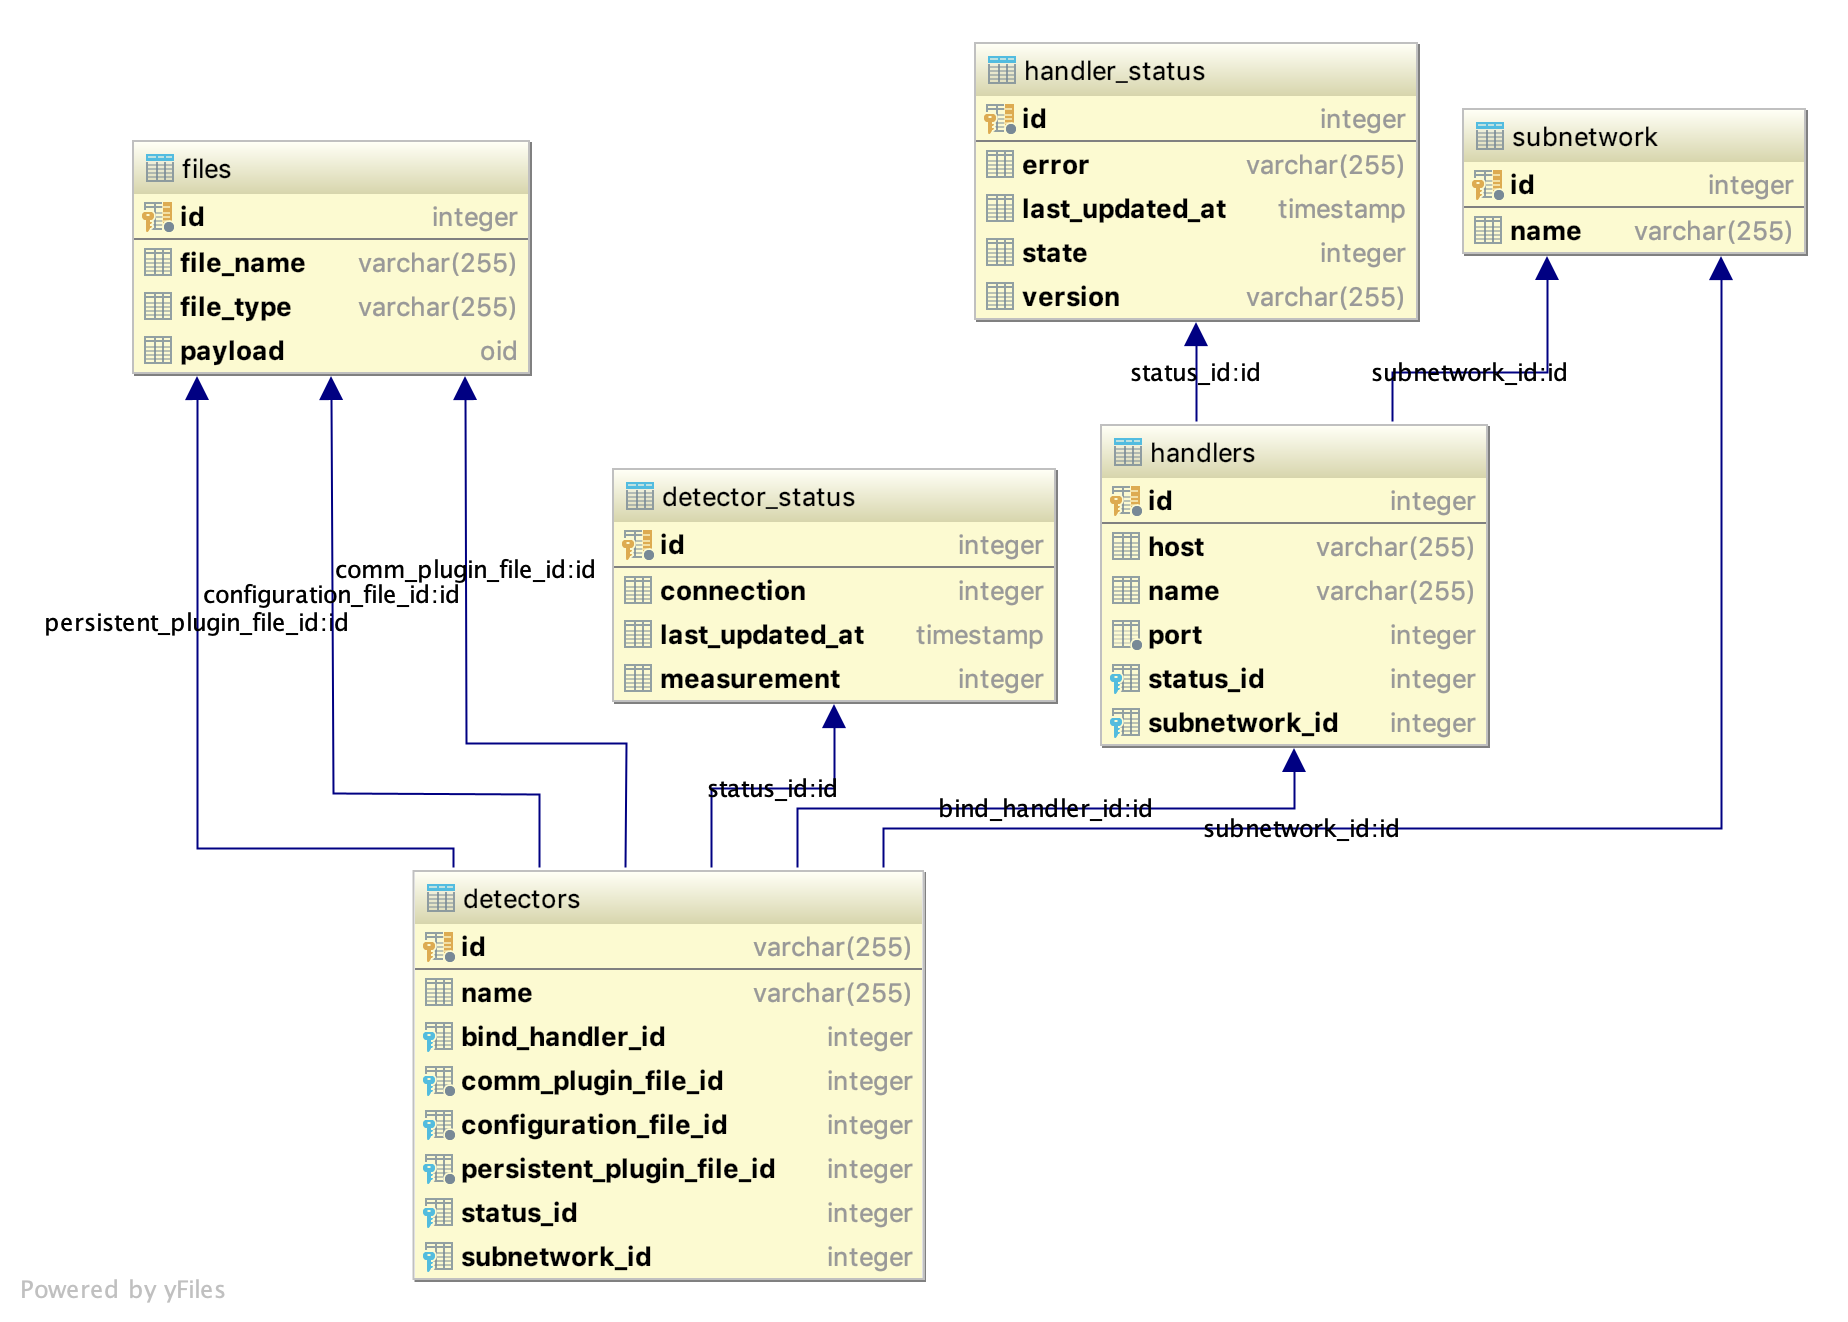
\includegraphics[width=15cm]{figures/master_db.png}
		\caption{Pixnet -- master: databázové schéma.}
		\label{fig:master:db_schema}
	\end{center}
\end{figure}

\subsection{Konfigurace a nasazení}
Pro spuštění mastera je třeba mít nainstalované \texttt{JRE 8}\footnote{\textit{Java SE Runtime Environment, dostupné z\\\url{https://www.oracle.com/technetwork/java/javase/downloads}}.} nebo vyšší.
Zkompilovanou java aplikaci je třeba spustit s argumentem \texttt{masterConfig} obsahující cestu ke konfiguračnímu souboru (pro příklad viz zdrojový kód \ref{src:master:config}), obsahujícího port na kterém bude aplikace naslouchat příchozí spojení.

Aplikaci je tedy možné spustit například takto: \mint{bash}{java -jar master.jar masterConfig=config.yaml}

\begin{code}[h]
  \begin{minted}[
  frame=single,
  linenos,
  breaklines
  ]{yaml}
# Connection parameters
portToListen: 8080
\end{minted}
\caption{\texttt{YAML} konfigurační soubor mastera.}
\label{src:master:config}
\end{code}

%********************************************************************************
% Frontend
%********************************************************************************
\section{Frontend}\label{chap:master:frontend}
Pomocí frameworku \textit{ReactJS} (viz \ref{chap:arch:technologie:react}) byl implementován webový klient, který implementuje API, poskytované backendovou aplikací mastera (viz \ref{chap:master:backend:sw_arch:api}). 

Jedná se o tzt. \textit{single-page} aplikaci, tj. aplikaci která načte jednu stránku, kterou pak dynamicky aktualizuje dle interakcí uživatele (ev. dalších událostí) bez nutnost stahování nové stránky ze serveru. Jak již bylo vysvětleno v kapitole \ref{chap:arch:technologie:react}, každá \textit{ReactJS} aplikace je založena na komponentách. Každá komponenta má svoje vlastnosti a svůj stav. Komponenty lze opětovně používat a je možné je libovolně zapouzdřovat. Při aktualizaci stavu některé z komponent, \textit{ReactJS} framework změnu detekuje a provede překreslení afektovaných částí uživatelského rozhraní.

Pro navigaci po stránce aplikace používá knihovnu \textit{react-router}\footnoteUrl{https://reacttraining.com/react-router/web}, která mění obsah stránky renderováním těchto komponent:

\begin{description}
    \item[Subnetworks] -- komponenta vizualizující seznam podsítí a umožňuje přidávání nových podsítí a odebírání existujících.
    \item[Handlers] -- tato komponenta zobrazuje seznam přidaných handlerů, včetně podseznamu jim přiřazených detektorů, stavu apod. Komponenta rovněž umožňuje přidání nových hadlerů a odstranění existujících. Pro screenshot viz obr. \ref{fig:master:frontend:handlers}.
    \item[Detectors] -- komponenta zobrazující seznam všech detektorů (viz \ref{fig:master:frontend:detectors}). Dále umožňuje přidávání nových detektorů a odebírání existujících.
    \item[Detector detail] -- komponenta s detailem detektoru (viz obr. \ref{fig:master:frontend:detector_detail}). Komponenta uživateli nabízí všechny operace nad detektorem, nabízené API backendové aplikace mastera (tj. např. přiřazování detektoru dostupnému handleru, navazování spojení s detektorem, vykonávání jeho příkazů apod.).
\end{description}

\begin{figure}[h]
	\begin{center}
        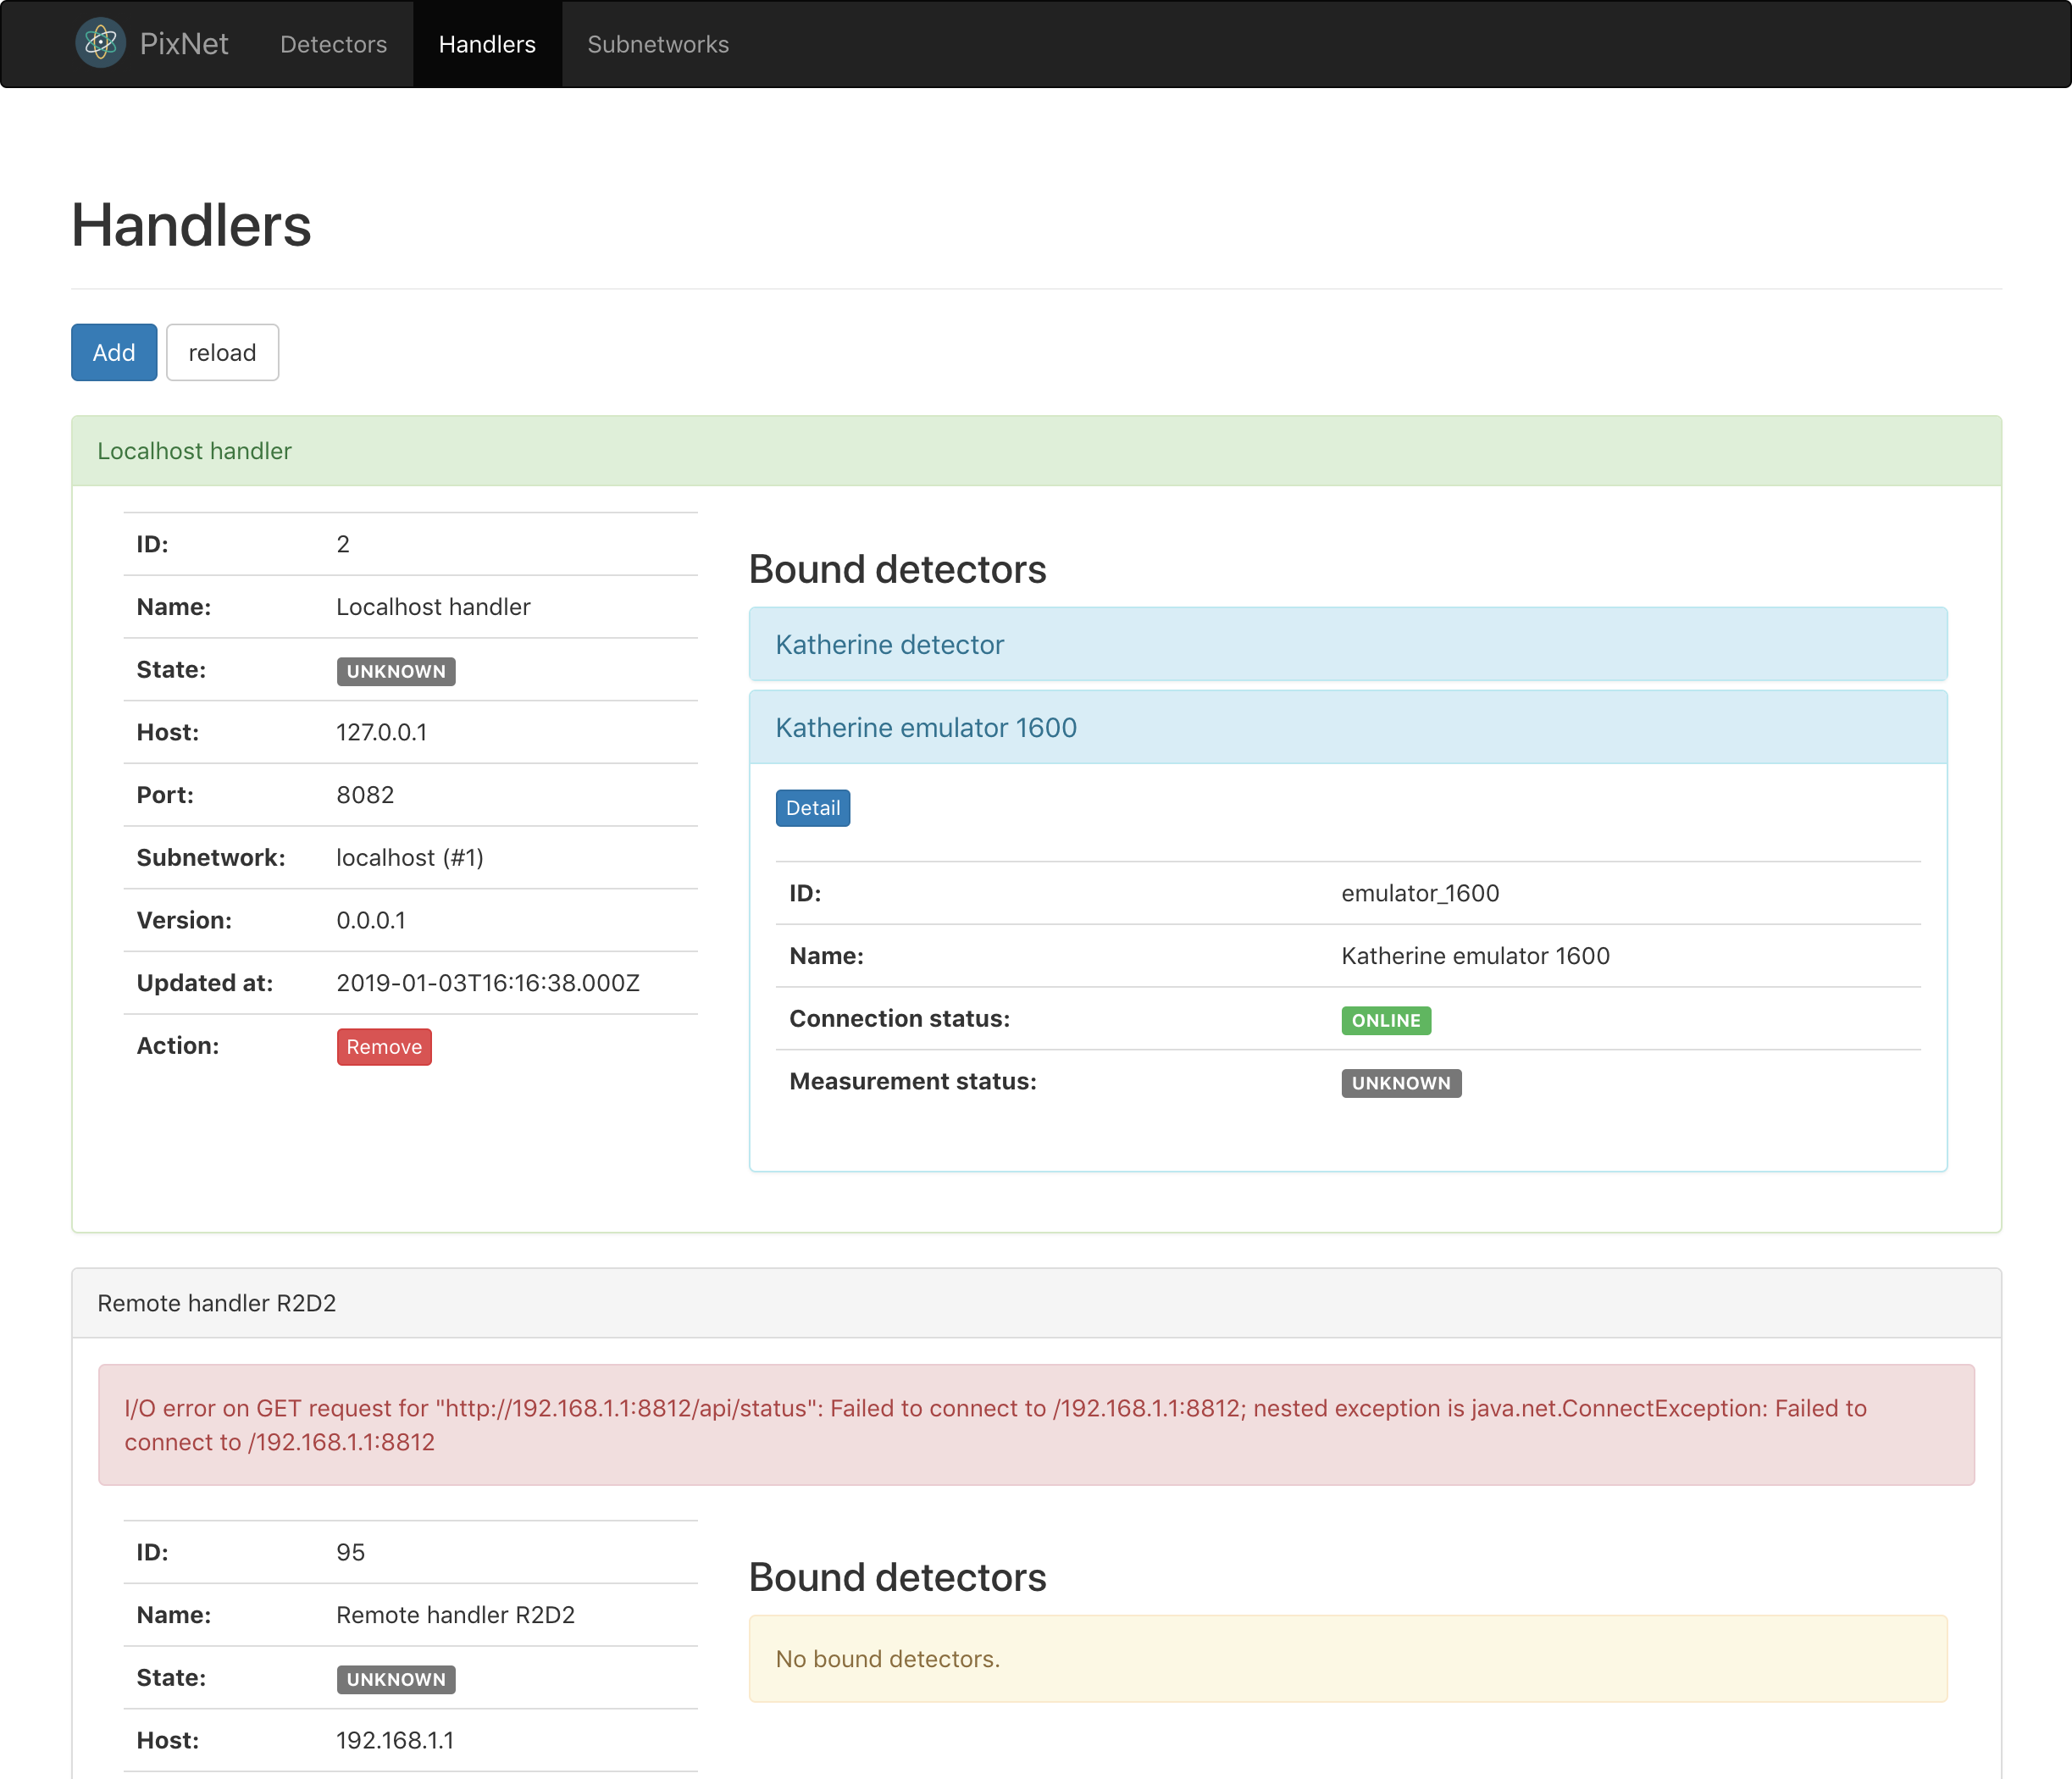
\includegraphics[width=15cm]{figures/master_handlers.png}
	\end{center}
	\caption{Master -- frontend: screenshot seznamu handlerů, dostupného z endpointu \texttt{/handlers}.}
	\label{fig:master:frontend:handlers}
\end{figure}

\begin{figure}[h]
	\begin{center}
        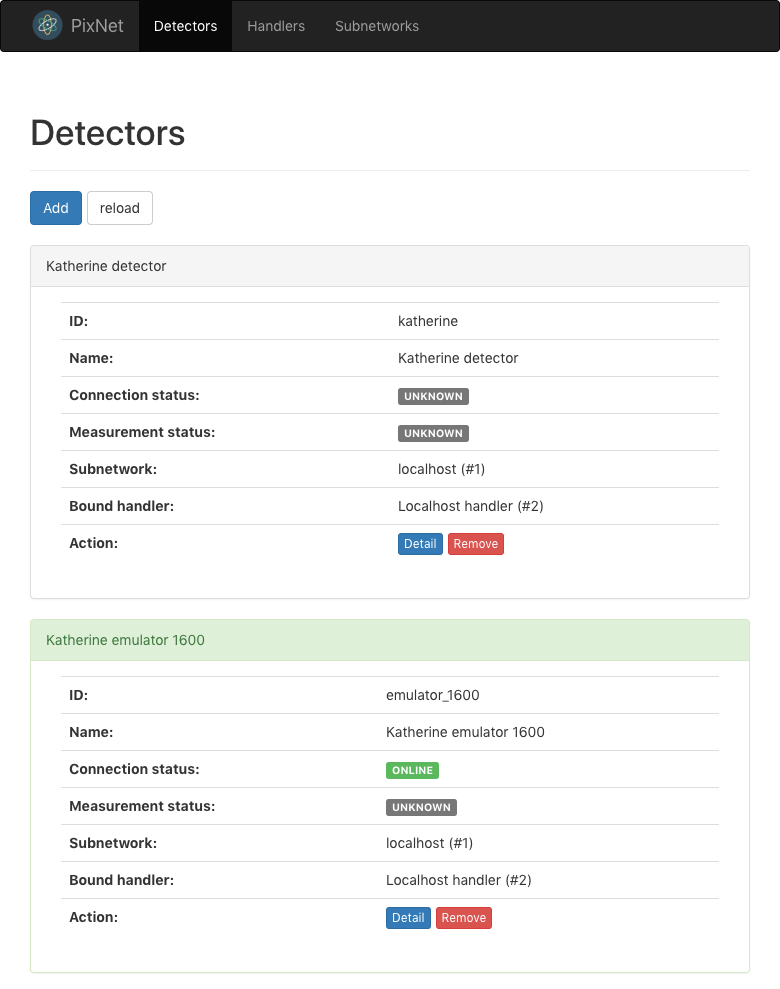
\includegraphics[width=10cm]{figures/master_detectors.png}
	\end{center}
	\caption{Master -- frontend: screenshot seznamu detektorů, dostupného z endpointu \texttt{/detectors}.}
	\label{fig:master:frontend:detectors}
\end{figure}

\begin{figure}[h]
	\begin{center}
        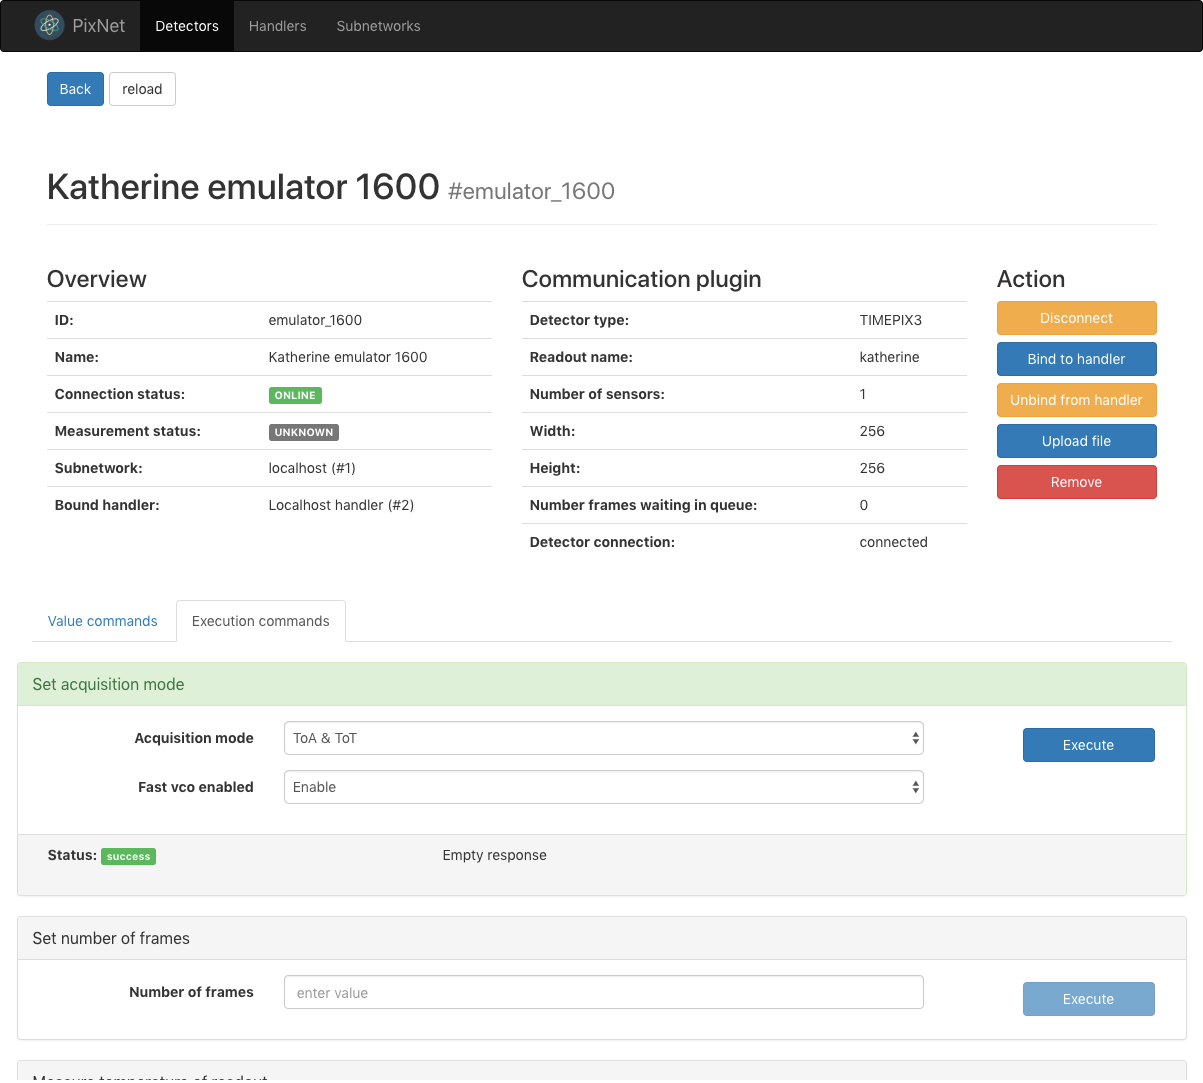
\includegraphics[width=15cm]{figures/master_detector_detail.png}
	\end{center}
    \caption{Master -- frontend: screenshot detailu detektoru, dostupného z endpointu \texttt{detectors/\{ID detektoru\}}.}
	\label{fig:master:frontend:detector_detail}
\end{figure}

\subsection{Nasazení}
Nasazení aplikace je jednoduché -- stačí jenom její build (k dispozici na přiloženém CD) nahrát na webový server. Build obsahuje \texttt{index.html} společně s vlastní aplikací v \texttt{bundle.js} a dalšími soubory (obrázky, CSS styly apod.).

Aplikace byla vyvinuta pomocí systému na správu závislostí \texttt{Yarn}\footnoteUrl{https://yarnpkg.com}. Pro vývojové účely je možné aplikaci spustit příkazem \texttt{yarn start}, nebo příkazem \texttt{yarn build} je možné udělat build aplikace, nasaditelný na webový server.
\addbibresource{reference.bib}

\chapter{Testování}\label{chap:test}
V této kapitol bude čtenář seznámen s metodami testování pro zajištění kvality jednotlivých softwarových komponent a s provedenými experimenty.

%********************************************************************************
% Metody testování
%********************************************************************************
\section{Metody testování}
\subsection{Jednotkové testy}
Pro části jednotlivých softwarových komponent byly použity jednotkové testy \cite{testing_evans} (tzv. \textit{Unit testy}). Jednotkové testy jsou základním typem testu, který ověřuje funkčnost samostatně testovatelných částí systému - tzv. jednotek. Výhodou těchto testů je jejich automatizovatelnost. Byl použit \textit{JUnit} framework - framework pro jednotkové testy pro platformu Java. 

\subsection{Integrační testy}
Integrační testy byly použity pro ověření správné komunikace jednotlivých komponent systému, zejména pak handlera (viz \ref{chap:handler}) a backendové aplikace mastera (viz \ref{chap:master:backend}), vyčítacího rozhraní \textit{Katherine} a komunikačního modulu apod.

V rámci těchto testů byla ověřována především správnost implementace komunikačního protokolu vyčítacího rozhraní \textit{katherine} (resp. její serverové implementace v emulátoru i implementace klienta v komunikačním modulu) a REST API handlera a mastera.

\subsection{Systémové testy}
Systémové testy se provádějí pro ověření funkčnosti systému jako celku. Tyto testy se provádějí až v pozdějších fázích vývoje a testují funkčnost systému z pohledu uživatele. Za tímto účelem bylo definováno několik testovacích scénářů (jako např. přidání detektoru do systému, přiřazení detektoru handleru, spuštění akvizice apod.), pomocí kterých byly tyto testy realizovány.

%********************************************************************************
% Experimenty
%********************************************************************************
\section{Experimenty}
Pro ověření funkčnosti a dostatečné propustnosti systému bylo provedeno několik experimentů, které budou v této podkapitole popsány. Pro tyto experimenty byla použita dvě různá prostředí:
\begin{description}
    \item[lokální] -- jeden počítač, na kterém byl spuštěn emulátor, handler a master současně. Použitý počítač má CPU 3 GHz Intel Core i7, 16 GB 1600 MHz DDR3 RAM a SSD disk o kapacitě \unit{500}{GB} (MacBook Pro).
    \item[CERN openstack] -- cloudová infrastruktura v CERN, kterou CERN poskytuje partnerským univerzitám a dalším institucím. Tato infrastruktura je založená na \textit{OpenStack} \textit{IaaS}\footnote{Z angl. \textit{Infrastructure as a Service}.} platformě, která umožňuje řízení výpočetního výkonu, úložiště a síťových prostředcích v datacentrech skrze webovou aplikaci nebo \textit{OpenStack API}.

    Byl vytvořen cluster s těmito virtuálními počítači:
    \begin{itemize}
        \item \texttt{pixnet-master.cern.ch} -- na tomto uzlu byla nasazena backendová aplikace mastera společně s webovým serverem, poskytujícím webový frontend mastera. Instance má 2~VCPU, \unit{4}{GB}~RAM a \unit{20}{GB} diskové kapacity.
        \item \texttt{pixnet-handler-1.cern.ch} -- uzel pro nasazení backendové aplikace handlera. Instance má 4~VCPU, \unit{8}{GB}~RAM a \unit{40}{GB} diskové kapacity.
        \item \texttt{pixnet-emulator-katherine1.cern.ch} -- uzel pro nasazení emulátoru vyčítacího rozhraní \textit{Katherine}. Instance má 1~VCPU, \unit{2}{GB}~RAM a \unit{10}{GB} diskové kapacity.
        \item \texttt{pixnet-emulator-katherine2.cern.ch} -- uzel pro nasazení emulátoru vyčítacího rozhraní \textit{Katherine}. Instance má 1~VCPU, \unit{2}{GB}~RAM a \unit{10}{GB} diskové kapacity.
    \end{itemize}

\end{description}

%********************************************************************************
% Experimenty - Experiment první
%********************************************************************************
\subsection{Experiment první: zpracovávání fronty naměřených dat}
Kritickou částí každého datového akvizičního systému je proces zpracování dat, od přijetí až po jejich uložení. Jelikož v rámci systému Pixnet data procházejí pouze přes handler (resp. od komunikačního do datového modulu daného detektoru, zavedených v handleru) do datovým modulem definovaného úložiště, budou v rámci tohoto experimentu zkoumány jen metadata jednotlivých událostí (od jejich vzniku až po uložení).

Experiment byl proveden v obou prostředích, v každém s jedním emulátorem vyčítacího rozhraní \textit{Katherine}, jedním handlerem a masterem. Byly sledovány dva parametry - čas zpracování události (tj. doba od jeho přijetí komunikačním modulem až po jeho uložení datovým modulem) a aktuální počet událostí ve frontě. Pro všechna měření byl emulátor nastaven tak, aby generoval fixní počet událostí za sekundu. Jako vyčítací mód emulátoru byl použit \textit{Data-Driven} (viz \ref{chap:detectors:readout}), akviziční mód byl \textit{ToA \& TOT} a délka akvizice byla vždy \unit{60}{s}. Na obr. \ref{fig:test:exp1:jedna_akvizice_50k_udalosti} je znázorněn průběh jednoho měření, při kterém emulátor generoval 50000 událostí za vteřinu, který zaznamenává vývoj doby zpracovávání událostí a velikosti fronty v čase.

\begin{figure}[h]
    \centering
    \begin{tikzpicture}
        \begin{axis}[
          xmin = 0, xmax = 62000,
          ymin = 0,
          axis y line*=left,
          xlabel={Čas [ms]},
          xlabel near ticks,
          ylabel={Doba zpracování událostí [ns]},
          ylabel near ticks,
          width=0.90\textwidth,
          height=0.89\textwidth,
        ]
          \addplot[color=orange] table {figures/data/test_queue_waiting.dat};
          \label{plot_1_y1}
        \end{axis}
        \begin{axis}[
          xmin = 0, xmax = 62000,
          ymin = 0,% ymax = 11000,
          hide x axis,
          axis y line*=right,
          ylabel={Počet událostí ve frontě},
          ylabel near ticks,
          width=0.90\textwidth,
          height=0.89\textwidth,
        ]
        \addplot[color=gray] table {figures/data/test_queue_size.dat};
        \label{plot_1_y2}
        \addlegendimage{/pgfplots/refstyle=plot_1_y1}\addlegendentry{Doba zpracování událostí}
        \addlegendimage{/pgfplots/refstyle=plot_1_y2}\addlegendentry{Počet událostí ve frontě}
        \end{axis}
      \end{tikzpicture}

    \caption{Vývoj doby zpracovávání událostí a počtu událostí ve frontě v rámci \unit{60}{s} dlouhé akvizice, při konstantním generovaném množství událostí ($50000~s^{-1}$).}
    \label{fig:test:exp1:jedna_akvizice_50k_udalosti}
\end{figure}

Měření byla provedena pro různé počty generovaných událostí za vteřinu (1, 10, 100, 1000, 10000, 25000, 50000, 75000 a 100000), ze kterých byla stanovena průměrná doba zpracovávání události v závislosti na počtu příchozích dat (viz obr. \ref{fig:test:exp1:zavyslost_na_poctu_udalosti:doba_zpracovani}) a průměrná velikost fronty v závislosti na počtu příchozích dat (viz obr. \ref{fig:test:exp1:zavyslost_na_poctu_udalosti:velikost_fronty}). Jednotlivá měření byla vícekrát zopakována a jejich dílčí hodnoty byly zprůměrovány. Maximální testovaný počet generovaných událostí za vteřinu byl 100000, kvůli omezení emulátoru.

\begin{figure}[h]
    \centering
    \begin{subfigure}[t!]{0.47\textwidth}
        \begin{tikzpicture}
            \begin{loglogaxis}[
                xlabel={Počet událostí [$s^{-1}$]},
                ylabel={Prům. čas zpracovávání [ns]},
                legend pos=north west,
                ymajorgrids=true,
                grid style=dashed,
                width=\textwidth,
                height=\textwidth,
            ]
            \addplot[
                color=red,
                mark=triangle,
                ]
                coordinates {
                    (1,548539.5)
                    (10,327037.6097)
                    (100,171609.3892)
                    (1000,80747.81636)
                    (10000,428631.4967)
                    (25000,3616756.103)
                    (50000,43089381.58)
                    (75000,7572697.545)
                    (100000,10406080.54)
                };
            \addplot[
                color=blue,
                mark=square,
                ]
                coordinates {
                    (1,548539.5)
                    (10,327037.6097)
                    (100,171609.3892)
                    (1000,80747.81636)
                    (10000,150000.808)
                    (25000,933122.5602)
                    (50000,3242140.3333)
                    (75000,4674643.645)
                    (100000,27828674.3)
                };
            \legend{lokální,CERN openstack} 
            \end{loglogaxis}
        \end{tikzpicture}
        \caption{Závislost průměrné doby zpracování události na počtu událostí za sekundu.}
        \label{fig:test:exp1:zavyslost_na_poctu_udalosti:doba_zpracovani}
    \end{subfigure}
    \hspace{0.2cm}
    \begin{subfigure}[t!]{0.47\textwidth}
    
        \begin{tikzpicture}
            \begin{loglogaxis}[
                xlabel={Počet událostí [$s^{-1}$]},
                ylabel={Průměrná velikost fronty},
                legend pos=north west,
                ymajorgrids=true,
                grid style=dashed,
                width=\textwidth,
                height=\textwidth,
            ]
            \addplot[
                color=red,
                mark=triangle,
                ]
                coordinates {
                    (1,0.2)
                    (10,0.305699482)
                    (100,0.383944154)
                    (1000,0.525876461)
                    (10000,1.495)
                    (25000,26.53898305)
                    (50000,1061.88027)
                    (75000,136.5602007)
                    (100000,90.73529412)
                };
            \addplot[
                color=blue,
                mark=square,
                ]
                coordinates {
                    (1,0.2)
                    (10,0.305699482)
                    (100,0.383944154)
                    (1000,0.525876461)
                    (10000,1.464106845)
                    (25000,2.091973244)
                    (50000,3.854271357)
                    (75000,5.154103853)
                    (100000,12.20805369)
                };
            \legend{lokální,CERN openstack}
            \end{loglogaxis}
        \end{tikzpicture}
        \caption{Závislost průměrné velikosti fronty s událostmi na počtu událostí za sekundu.}
        \label{fig:test:exp1:zavyslost_na_poctu_udalosti:velikost_fronty}
        
    \end{subfigure}
        
    \caption{Závislost průměrné doby zpracování událostí a jejich průměrného počtu ve frontě na počtu událostí za sekundu.}
    \label{fig:test:exp1:zavyslost_na_poctu_udalosti}
\end{figure}

Z výsledku experimentu je patrné, že obě sledované hodnoty rostou s počtem událostí. Oproti očekávaným hodnotám (resp. očekávané rostoucí závislosti) lze z obr. \ref{fig:test:exp1:zavyslost_na_poctu_udalosti} pozorovat dva rozdíly. 

Tím prvním je vývoj průměrné doby zpracování události od jedné do 1000 událostí za sekundu. Tento efekt je pravděpodobně způsoben nastavenou velikostí \textit{bufferu} a režie přenosu dat.

Druhým rozdílem je různý trend hodnot pro \textit{CERN openstack} a \textit{lokání} prostředí od 50000 událostí za vteřinu. Nejvíce pravděpodobnou příčinou tohoto jevu je rozdílná konfigurace obou prostředí. Zatímco v rámci \textit{CERN openstack} každá komponenta systémů je spuštěna na jiném počítači, v \textit{lokální} prostředí všechny komponenty sdílí stejný počítač a vzájemně se ovlivňují.

%********************************************************************************
% Experimenty - Experiment druhý
%********************************************************************************
\subsection{Experiment druhý: zátěžový test API mastera}
V rámci tohoto experimentu byl proveden zátěžový test API mastera, který byl proveden v rámci \textit{lokálního} prostředí. Pomocí software \textit{Apache JMeter} bylo provedeno několik měření, ve kterých byl sledován čas zpracovávání requestu (resp. jeho průměr a medián) a průměrný počet zpracovaných událostí za minutu v závislosti na počtu simultánně přistupujících uživatelů. Experiment byl proveden pro 1, 10, 100, 500, 1000, 2000, 3000, 4000, 5000, 6000, 7000, 8000, 9000 a 10000 uživatelů, resp. použitých vláken. Každý experiment byl několikrát zopakován a výsledky byly zprůměrovány. 

Výsledek experimentu je zobrazen v obrázku \ref{fig:test:exp2}. Z grafu je patrné, že do zhruba 3000 simultánně přistupujících uživatelů počet zpracovaných uživatelů za minutu stoupá a při větším počtu uživatelů začíná klesat. 

Dále je patrné, že od zhruba 6000 simultánně přistupujících uživatelů průměrná doba zpracovávání requestu roste oproti jejího mediánu rychleji. To je dáno tím, že některé requesty nestihnou být serverem obslouženy v rámci daného \textit{timeout} a tím je negativně ovlivněna doba jejich zpracování.

Je třeba poznamenat, že měření bylo zatíženou chybou, protože měřící software byl spuštěn na stejném počítači, jako systém Pixnet. Měřící software vytváří velké množství vláken, simulující přistupující uživatele a Tomcat webový server mastera vytváří nová vlákna také, aby velké množství klientů mohl obsloužit.

\begin{figure}[h]
    \centering
    \begin{tikzpicture}
        \begin{axis}[
          xmin = 0,% xmax = 62000,
          ymin = 0, ymax = 2000,
          axis y line*=left,
          xlabel={Počet vláken},
          xlabel near ticks,
          ylabel={Čas zpracování requestu [ms]},
          ylabel near ticks,
          width=0.88\textwidth,
          height=0.89\textwidth,
        ]
            \addplot[color=orange,mark=triangle]
                coordinates {
                    (1,3)
                    (10,2)
                    (100,2)
                    (500,4)
                    (1000,4)
                    (2000,99)
                    (3000,176)
                    (4000,206)
                    (5000,217)
                    (6000,245)
                    (7000,430)
                    (8000,472)
                    (9000,324)
                    (10000,539)
                };
            \label{plot_2_y1}
            \addplot[color=gray,mark=asterisk]
                coordinates {
                    (1,3)
                    (10,2)
                    (100,2)
                    (500,3)
                    (1000,3)
                    (2000,59)
                    (3000,143)
                    (4000,179)
                    (5000,167)
                    (6000,235)
                    (7000,317)
                    (8000,190)
                    (9000,168)
                    (10000,219)
                };
            \label{plot_2_y2}
        \end{axis}
        \begin{axis}[
          xmin = 0,% xmax = 62000,
          ymin = 0,% ymax = 11000,
          hide x axis,
          axis y line*=right,
          ylabel={Počet requestů [$s^{-1}$]},
          ylabel near ticks,
          width=0.88\textwidth,
          height=0.89\textwidth,
          legend pos=north east,
        ]
        \addlegendimage{/pgfplots/refstyle=plot_2_y1}\addlegendentry{Avg [ms]}
        \addlegendimage{/pgfplots/refstyle=plot_2_y2}\addlegendentry{Med [ms]}
        \addplot[color=blue,mark=square]
                coordinates {
                    (1,53)
                    (10,662)
                    (100,5870)
                    (500,20732)
                    (1000,33127)
                    (2000,41011)
                    (3000,58100)
                    (4000,54066)
                    (5000,60851)
                    (6000,56426)
                    (7000,57731)
                    (8000,47477)
                    (9000,49222)
                    (10000,40222)
                };
            \addlegendentry{Thr [$min^{-1}$]}
        \end{axis}
      \end{tikzpicture}

    \caption{Závislost počtu zpracovávaných requestů za minutu (v legendě jako \textit{Thr}, pravá osa) na počtu vláken a závislost času zpracovávání requestu (znázorněno jako \textit{Avg} (průměr) a \textit{Med} (medián), levá osa) na počtu vláken.}
    \label{fig:test:exp2}
\end{figure}
\addbibresource{reference.bib}

\chapter{Závěr}\label{chap:zaver}
Cílem této práce bylo navrhnout a implementovat distribuovaný systém, který bude schopný řídit a vyčítat data ze sítě hybridních částicových pixelových detektorů \textit{Timepix3} za pomocí vyčítacího rozhraní \textit{Katherine}. 

Výsledkem této práce je modulární distribuovaný systém, který uživateli umožňuje operovat teoreticky neomezené množství detektorů různých typů. Implementovaný systém se skládá ze dvou hlavních komponent - handlera a mastera.

\textbf{Handler} slouží pro komunikaci s detektory a vyčítání dat z jemu přiřazených detektorů do uživatelem definovaném datovém úložištěm. Díky modulární architektuře je možné handleru přiřadit detektory různých typů a jimi naměřená data zpracovávat rozdílnými způsoby (např. odesílat do různých datových úložišť apod.). Komponenta také poskytuje jednoduché webové rozhraní a také \textit{API} pro své řízení jinými komponentami systému, ev. možnost integrace do systémů třetích stran. Počet detektorů, které je možné jednomu handleru přiřadit, je dán sumou jejich datového toku, komplexitou zpracovávání naměřených dat a hardwarovou konfigurací počítače, na kterém je instance handleru nasazena.

\textbf{Master} je centrálním elementem systému, jehož hlavním úkolem je řízení všech handlerů sítě pomocí jejich \textit{API}. Komponenta rovněž implementuje perzistentní úložiště konfigurace a stavu systému. Master dále poskytuje \textit{API} pro své řízení. Primárním konzumentem \textit{API} je webový frontendový klient, který byl implementován jako \textit{single-page} aplikace, která uživateli poskytuje uživatelské rozhraní pro plnohodnotné řízení celého systému. Pomocí \textit{API} mastera může být systém rovněž integrován do systémů třetích stran, jako např. pro účely experimentu \textit{ATLAS-TPX} se systémem \texttt{DCS} (CERN systémem pro řízení a akvizici dat detektorových systémů).

Výše zmíněná modulární architektura spočívá v možnosti operování různých typů detektorů. Při přidávání detektoru do systému je uživatel nucen poskytnout také jeho komunikační a datový modul. Komunikační modul musí obsahovat implementaci komunikačního interface (popsaného v \ref{chap:handler:detector_layer:commIntf}) a datový modul musí zase obsahovat implementaci datového interface (viz \ref{chap:handler:detector_layer:dataIntf}).

V rámci této práce byl rovněž vyvinut komunikační a datový modul, jehož prostřednictvím je možné řídit a vyčítat naměřená data z vyčítacího rozhraní \textit{Katherine}, s připojeným \textit{Timepix3} detektorem. Implementovaný datový modul pak umožňuje ukládání dat ve formě souborů do uživatelem definovaného úložiště (např. do distribuovaného souborového systému, jako je např. \texttt{HDFS} (\textit{Hadoop Distributed File System})), nebo do \textit{MongoDB} distribuovatelné dokumentové databáze.

Pro účely vývoje a testování byl rovněž vyvinut \textbf{emulátor} vyčítacího rozhraní \textit{Katherine}, který emuluje zařízení na síťové vrstvě. Emulátor implementuje všechny příkazy, které jsou důležité pro konfiguraci a spuštění akvizice dat (jako např. nastavení biasu, akvizičního času, vyčítacího a měřícího módu apod.). Emulátor je schopný generovat náhodná data (resp. události vzniklé interakcí s ionizujícím zářením) všech možných kombinací, daných akviziční konfigurací.

%********************************************************************************
% Budoucí vývoj
%********************************************************************************
\section{Budoucí vývoj}
\subsection{Podpora více datových modulů jedním detektorem}
V kapitole \ref{chap:arch:sw:detector} bylo popsáno, že instance detektoru v handleru je tvořena jeho komunikačním a datovým modulem, které jsou při inicializaci detektoru propojeny asynchronní frontou s naměřenými daty. Tato modifikace systému spočívá v možnosti přidání dalších konzumentů fronty - vícero datových modulů. Tento přístup umožňuje jednoduché přidání dalších komponent pro zpracování dat, např. komponentu pro analýzu naměřených dat v reálném čase, simultánní nahrávání dat do více datových současně apod.

\subsection{Podpora pro analýzu a vizualizaci dat v reálném čase}
Možnost zobrazení naměřených dat je pro operátora systému důležitá pro zajištění kvality měřených dat a ověření konfigurace systému. 

Je plánováno přidání podpory pro umožnění poskytovateli komunikačního modulu, aby si definoval důležité hodnoty, které budou v reálném čase sledovány (např. okupance snímků, teploty apod.). Tyto hodnoty pak budou masterem v pravidelných intervalech vyčítány, ukládány a budou poskytovány pomocí jeho \textit{API}. Webová aplikace pak bude nabízet vizualizaci vývoje těchto sledovaných hodnot v závislosti na čase.

Rovněž je plánováno přidání podpory pro vizualizaci dat z datového úložiště, ev. výsledky \textit{real-time} analýzy dat.

\subsection{Zabezpečení}
Před nasazením do produkce je plánováno přidání zabezpečení endpointů, poskytovaným \textit{API} handlera (pravděpodobně pomocí \textit{Base64}, protože \textit{API} handlera má jediného konzumenta - mastera). \textit{API} mastera bude zabezpečeno pomocí průmyslového standardu \textit{OAuth2}, protože je plánován přístup více klientů, kterými jsou uživatelé webové aplikace a ev. systémy třetích stran. Autentizace uživatelů bude rovněž implementována v rámci webové aplikace.

\subsection{Podpora vyčítacího rozhraní ATLAS Pix}
V kapitole \ref{chap:detectors:readouts:atlaspix} bylo zmíněno vyčítací rozhraní \textit{ATLAS~Pix}, pomocí kterého je v současné době realizována detektorová siť \textit{ATLAS-TPX}. Pro zajištění zpětné kompatibility s existujícím systému (resp. možnost operování i detektorů s \textit{ATLAS~Pix} rozhraním), bude implementován komunikační modul pro řízení a vyčítání dat z těchto zařízeních.

\subsection{Podpora modifikovaného vyčítacího rozhraní Katherine pro řízení detektorů Timepix2}
V současné době je dokončován vývoj nového detektoru \textit{Timepix2}, pro který je vyvíjena modifikace vyčítacího rozhraní \textit{Katherine}. Je plánováno vytvoření komunikačního modulu pro toto zařízení, modifikací existujícího komunikačního modulu, již vyvinutého pro původní \textit{Katherine}.

\bibliographystyle{csplainnat}

{
%JZ: 11.12.2008 Kdo chce mit v~techto ukazkovych odkazech take odkaz na CSTeX:
\def\CS{$\cal C\kern-0.1667em\lower.5ex\hbox{$\cal S$}\kern-0.075em $}
\bibliography{reference}
}


%%%%%%%%%%%%%%%%%%%%%%%%%% 
% Přílohy
\appendix	
%\chapter{Závislosti modulu Handler}\label{chap:app:handler_dependencies}
\chapter{Přílohy vyčítacího rozhraní Katherine}\label{chap:app:katherine}

\section{Přehled DAC vyčítacího rozhraní Katherine}\label{chap:app:katherine:dacs}
\begin{table}[h]
	\begin{center}
		\begin{tabular}{|c|c|c|}
			\hline
            \textbf{Název} & \textbf{ID pro čtení} & \textbf{ID pro zápis} \\
			\hline
            Ibias\_Preamp\_ON & 1 & 0 \\
            Ibias\_Preamp\_OFF & 2 & 1 \\
            VPreamp\_NCAS & 3 & 2 \\
            Ibias\_Ikrum & 4 & 3 \\
            Vfbk & 5 & 4 \\
            Vthreshold\_fine & 6 & 5 \\
            Vthreshold\_coarse & 7 & 6 \\
            Ibias\_DiscS1\_ON & 8 & 7 \\
            Ibias\_DiscS1\_OFF & 9 & 8 \\
            Ibias\_DiscS2\_ON & 10 & 9 \\
            Ibias\_DiscS2\_OFF & 11 & 10 \\
            Ibias\_PixelDAC & 12 & 11 \\
            Ibias\_TPbufferIn & 13 & 12 \\
            Ibias\_TPbufferOut & 14 & 13 \\
            VTP\_coarse & 15 & 14 \\
            VTP\_fine & 16 & 15 \\
            Ibias\_CP\_PLL & 17 & 16 \\
            PLL\_Vcntrl & 18 & 17 \\
            BandGap output & 28 & - \\
            BandGap\_Temp & 29 & - \\
            Ibias\_dac & 30 & - \\
            Ibias\_dac\_cas & 31 & - \\
			\hline
		\end{tabular}
	\end{center}
	\caption{Přehled DAC (digitálně analogových převodníků) vyčítacího rozhraní katherine.}
	\label{tab:app:dacs}
\end{table}

\section{Přehled HW příkazů vyčítacího rozhraní Katherine}\label{chap:app:katherine:hw_commands}
\begin{table}[h]
	\begin{center}
		\begin{tabular}{|c|l|}
			\hline
            \textbf{ID} & \textbf{Název} \\
			\hline
            0 & Sensor Config Registers Update \\
            1 & Internal DAC Update \\
            2 & Internal DAC Back Read \\
            3 & Timer Read \\
            4 & Timer Set \\
            5 & Reset Matrix Sequential \\
            6 & Stop Matrix Command \\
            7 & Load Column Test Pulse Register \\
            8 & Read Column Test Pulse Register \\
            9 & Load Pixel Register Configuration \\
            10 & Read Pixel Register Configuration \\
            11 & Read Pixel Matrix Sequential Setting \\
            12 & Read Pixel Matrix Data-Driven Setting \\
            13 & Chip ID Read \\
            14 & Output Block Config Update \\
            15 & Digital Test \\
			\hline
		\end{tabular}
	\end{center}
	\caption{Přehled HW příkazů vyčítacího rozhraní katherine.}
	\label{tab:app:hw_commands}
\end{table}

\section{Přehled registrů detektoru Timepix3 v rámci vyčítacího rozhraní Katherine}\label{chap:app:katherine:tpx3_registers}
\begin{table}[h!]
	\begin{center}
		\begin{tabular}{|c|l|}
			\hline
            \textbf{ID} & \textbf{Název} \\
			\hline
            0 & Test Pulse Period \\
            1 & Number Test Pulses \\
            2 & Out Block Config \\
            3 & PLL Config \\
            4 & General Config \\
            5 & SLVS Config \\
            6 & Power Pulsing Pattern \\
            7 & SetTimer 15..0 \\
            8 & SetTimer 31..16 \\
            9 & SetTimer 47..32 \\
            10 & Sense DAC Selector \\
            11 & Ext DAC Selector \\
			\hline
		\end{tabular}
	\end{center}
	\caption{Přehled registrů detektoru Timepix3 v rámci vyčítacího rozhraní Katherine.}
\end{table}

\section{Konfigurace pixelů detektoru}\label{chap:app:katherine:pix_config}
\begin{code}[h!]
\begin{minted}[
frame=single,
linenos,
breaklines
]{Kotlin}
fun bmcToMatrixConfig(bmc: ByteArray): ByteArray {
    assert(bmc.size == 65536)
    val buff = IntArray(16384)

    for (i in bmc.indices) {
        var y = i / 256
        val x = i % 256
        val tmp = bmc[i]
        y = 255 - y
        buff[64 * x + (y shr 2)] = buff[64 * x + (y shr 2)] or (tmp.toInt() shl 8 * (3 - y % 4))
    }

    val out = ByteArray(65536)
    var k = 0
    for (mem in buff) {
        val b = ByteBuffer.allocate(4).putInt(mem).array()
        for (i in 0..3) {
            out[k + 3 - i] = b[i]
        }
        k += 4
    }

    return out
}
\end{minted}
\caption{Ukázka kódu pro převod pixelové konfigurace detektoru z formátu \texttt{BMC} do formátu podporovaného vyčítacím rozhraním \textit{Katherine}.}
\end{code}

\printnomenclature
\label{apx:zkratky}

\chapter{Obsah přiloženého CD}\label{chap:app:cd}

\definecolor{fblue}{RGB}{92,144,192}
\definecolor{fgreen}{RGB}{34,162,70}

\def\Size{4pt}
\newcommand\myfolder[2][fblue]{%
\begin{tikzpicture}[overlay]
%\begin{scope}[xshift=20pt]
%\tikzset{
\filldraw[draw=folderborder,top color=folderbg!50,bottom color=folderbg]
      (-1.05*\Size,0.2\Size+5pt) rectangle ++(.75*\Size,-0.2\Size-5pt);  
    \filldraw[draw=folderborder,top color=folderbg!50,bottom color=folderbg]
      (-1.15*\Size,-\Size) rectangle (1.15*\Size,\Size);
%\end{scope}  
\end{tikzpicture}%
\makebox[2cm]{\raisebox{-3pt}{{\ttfamily#2}}}%
%}
}


\begin{figure}[th!]
\begin{center}
\begin{forest}
  for tree={
    font=\ttfamily,
    grow'=0,
    child anchor=west,
    parent anchor=south,
    anchor=west,
    calign=first,
    inner xsep=7pt,
    edge path={
      \noexpand\path [draw, \forestoption{edge}]
      (!u.south west) +(7.5pt,0) |- (.child anchor) \forestoption{edge label};
    },
    before typesetting nodes={
      if n=1
        {insert before={[,phantom]}}
        {}
    },
    fit=band,
    before computing xy={l=15pt},
  }  
[CD/
	[pixnet/
		[commons/ - modul se společnými závislosti]
		[detector\_communication\_intf/ - modul s komunikačním interface]
		[detector\_communication\_katherine/ - komunikační modul Katherine]
		[detector\_data\_persistence\_intf/ - modul s datovým interface]
		[handler/ - modul s handlerem]
		[katherine\_commons/ - společné závislosti Katherine modulů]
		[katherine\_emulator/ - emulátor Katherine]
		[katherine\_persistence\_file/ - datový modul Katherine]
		[master/ - modul s backendovou aplikací mastera]
	]
	[pixnet\_frontend/ - webová single-page aplikace]
	[text/
		[src/ - adresář se zdrojovými soubory tohoto dokumentu]
		[master-thesis-jakub-begera-2019.pdf - tato práce ve formátu PDF]
		[abstract\_cz.txt - abstrakt česky]
		[abstract\_en.txt - abstrakt anglicky]
	]
	[detector\_model.json - přehled příkazů komunikačního modulu Katherine]
]
\end{forest}
\end{center}
\caption{Obsah přiloženého CD}
\label{fig:attached-cd}
\end{figure}

\end{document}
